% V8.3.1 — derived from V8.3.0 (MDPI APA template)
\documentclass[apajournal,article,submit,moreauthors]{Definitions/mdpi}

% MDPI internal metadata (keep, may be empty)
\firstpage{1}
\makeatletter
\setcounter{page}{\@firstpage}
\makeatother
\pubvolume{1}
\issuenum{1}
\articlenumber{0}
\pubyear{2026}
\copyrightyear{2026}
\datereceived{}
\daterevised{}
\dateaccepted{}
\datepublished{}

% Pandoc helpers
\providecommand\tightlist{}
\newcommand\real[1]{#1}
\providecommand{\pandocbounded}[1]{#1}

% Fix fancyhdr headheight warning (MDPI template default is too small)
\setlength{\headheight}{20.0pt}
\addtolength{\topmargin}{-8.0pt}

% Packages needed by pandoc tables
\usepackage{longtable}
\usepackage{booktabs}
\usepackage{array}
\usepackage{float}
\usepackage{graphicx}
\usepackage{xurl}  % allow URLs to break across lines at any character
\setkeys{Gin}{width=0.95\linewidth,keepaspectratio}
\usepackage{caption}
\captionsetup[figure]{labelfont=bf,labelsep=period,skip=8pt,belowskip=4pt}

\Title{Personality-Adaptive Conversational AI for Emotional Support: A Simulation Study Integrating Big Five Detection with Zurich Model Regulation}
\Author{Jiahua Duojie $^{1}$, Samuel Devdas $^{1}$, Dr.~Guang Lu $^{1}$ and Dr.~Alexandre de Spindler $^{2}$*}
\AuthorNames{Jiahua Duojie; Samuel Devdas; Guang Lu; Alexandre de Spindler}
\address{%
$^{1}$ \quad Lucerne University of Applied Sciences and Arts (HSLU), 6002 Luzern, Switzerland; duojie.jiahua@stud.hslu.ch (J.~Duojie); samuel.devdas@hslu.ch (S.~Devdas); guang.lu@hslu.ch (G.~Lu)\\
$^{2}$ \quad Zurich University of Applied Sciences (ZHAW), 8400 Winterthur, Switzerland; alexandre.despindler@zhaw.ch}
\corres{Correspondence: alexandre.despindler@zhaw.ch}

\abstract{Many AI-driven digital mental health interventions rely on generic communication strategies and do not yet incorporate relatively stable personality differences that shape emotional processing and support preferences. We propose a theory-grounded personality-adaptive pipeline that performs turn-by-turn Big Five trait detection and applies Zurich Model-aligned behavioral regulation, orchestrated with PROMISE (a model-driven framework for state-based LLM orchestration) for traceable, reproducible control. We generated 20 simulated dialogue sessions (120 turns total) comparing regulated and non-adaptive conversational AI agents across two boundary-condition Big Five profiles (all traits set to +1 vs.~$-1$). Performance was assessed using a structured LLM-based evaluator complemented by author-conducted qualitative review. The system achieved high implementation fidelity (98.3\% detection accuracy; 100\% regulation adherence). In the regulated condition, personality needs were consistently addressed compared to minimal fulfillment in the baseline condition (8.3\%; Cohen's \(d\) = 4.42, \(p < 0.001\)), reflecting a \textbf{binary architectural difference} rather than a graded dose--response improvement. Emotional tone and relevance did not differ between conditions (\(d\) = 0.000 and \(d\) = 0.183, ns), confirming \textbf{selective enhancement} of personalization without degrading generic conversational quality. As this study is based on a synthetic simulation, real-world effect sizes are expected to be smaller (estimated \(d\) = 0.5--1.5). These findings provide a reproducible detection $\rightarrow$ regulation $\rightarrow$ evaluation framework for future empirical validation of personality-adaptive AI-augmented mental health support with human participants. As quantitative ratings were produced by an LLM-based evaluator and qualitative review was conducted by contributing authors, results should be interpreted as proof-of-concept evidence pending independent human-rater validation.}
\keyword{digital mental health; conversational agents; large language models; Big Five personality detection; Zurich Model}

\begin{document}
\section{Introduction}\label{introduction}

Mental health disorders have surged globally despite economic and technological progress, with loneliness contributing to morbidity risks comparable to obesity {[}1{]}. Population aging, dispersed families, and declining community engagement create unprecedented demand for scalable digital mental health interventions {[}2{]}.

Conversational AI agents for mental health support leveraging large language models (LLMs) have demonstrated capacity for emotionally relevant, context-aware responses {[}8,9{]}, yet a critical limitation persists: many current systems rely on generic or ``one-size-fits-all'' communication strategies and offer only shallow personalization {[}22--24,65,66{]}, while relatively stable personality differences---which shape how individuals process emotions, seek support, and respond to intervention styles {[}4{]}---are seldom incorporated or dynamically adapted {[}65,67{]}. Existing approaches typically use static assessments rather than continuous personality modeling grounded in psychological theory or dynamic adaptation throughout interactions.

To address these limitations, we developed a personality-adaptive conversational framework integrating: (i) real-time Big Five personality trait detection using continuous linguistic analysis, (ii) behavior regulation grounded in the Zurich Model of Social Motivation, explicitly mapping traits to security, arousal, and affiliation domains, and (iii) structured LLM-based evaluation with author-conducted qualitative review. Implemented using GPT-4 and the PROMISE orchestration system {[}7{]}---a model-driven framework that uses state machine modeling to compose prompts from modular parts, enforcing structured prompt/state control and traceable state transitions---the framework performs turn-by-turn personality inference and theory-guided behavioral adaptation throughout multi-turn conversations. The overarching framework was first conceived in prior work {[}68{]} (``a turn-by-turn detection--regulation pipeline for OCEAN-based behavioral adaptation in conversational AI, implemented with GPT-4 and PROMISE orchestration''); the present study extends that conception to a controlled factorial simulation with systematic statistical evaluation.

AI-driven digital interventions in mental health encompass software systems that embed AI techniques to deliver, support, or evaluate mental health services. While conversational AI agents show promise in providing accessible and scalable support, their effectiveness depends on moving beyond generic dialogue capabilities toward personalized interaction strategies grounded in psychological theory. This study contributes to this emerging landscape by demonstrating how relatively stable personality traits can inform adaptive regulation strategies that augment baseline LLM conversational quality with theory-driven personalization, rather than replacing generic competence.

This controlled simulation study tests whether real-time personality-adaptive regulation produces measurable improvements in AI-to-AI simulation compared to non-adaptive baselines across boundary-condition personality profiles. This design provides precise experimental control for quantifying personalization effects, establishes a reproducible methodological testbed, and validates the implementation approach as a foundation for future empirical studies with human participants toward safe, effective, and equitable AI-augmented mental health support. Our results demonstrate near-perfect implementation fidelity (98.3\% detection accuracy, 100\% regulation adherence) and a selective enhancement pattern: dramatic gains in personality-specific need fulfillment under regulation (100\% vs.~8.3\% baseline; Cohen's $d = 4.42$, $p < 0.001$) with no degradation of generic conversational quality, confirming the architectural feasibility of the D--R--E (Detection--Regulation--Evaluation) pipeline.

\section{Related Work}\label{related-work}

Personality-adaptive conversational AI sits at the intersection of affective computing, digital mental health interventions, personality-aware dialogue systems, and LLM-based conversational architectures. We synthesize this landscape in two arcs: (i) the evolution from emotion recognition to deployed support tools and personality-aware dialogue, and (ii) the rise of LLMs alongside the resulting orchestration and evaluation challenges.

\subsection{From Affective Computing to Personality-Aware Digital Support}\label{from-affective-computing-to-personality-aware-digital-support}

Early affective computing focused on recognizing transient emotional states from text, speech, and facial expressions {[}12,13{]}, evolving from categorical models toward dimensional representations (valence/arousal). A persistent limitation is the emphasis on short-lived states without incorporating relatively stable individual differences that shape how emotions are processed and how support is received {[}6{]}.

In parallel, commercial companions and research interventions (e.g., Replika, Woebot, ElliQ) demonstrate that conversational agents can deliver scalable support and reduce loneliness-related outcomes {[}21--24{]}. However, many systems remain ``one-size-fits-all,'' relying on fixed interaction strategies or shallow personalization based on preferences rather than stable psychological profiles {[}22--24{]}.

Personality-aware dialogue research suggests that adapting language style and interaction strategies to Big Five traits can improve perceived naturalness and engagement {[}6,30{]}. Yet most approaches rely on static initialization (explicit questionnaires or one-time inference) and do not update as evidence accumulates, limiting long-term consistency and attunement {[}6,30{]}.

To move beyond surface-level stylistic matching, computational systems also require a cognitive-motivational rationale for why traits should alter interaction strategies. The Zurich Model of Social Motivation {[}10,26--29{]} provides this grounding by linking Big Five traits to three motivational domains---security, arousal, and affiliation---offering a principled basis for mapping detected traits to regulation behaviors.

\subsection{LLMs in Mental Health: Capabilities and Evaluation Challenges}\label{llms-in-mental-health-capabilities-and-evaluation-challenges}

LLMs have transformed conversational AI by enabling flexible reasoning, context integration, and fluent natural language generation {[}8,15,16{]}. Instruction-tuned variants---trained to follow human-specified directives via reinforcement learning from human feedback---further improved controllability and alignment {[}64{]}. Recent work demonstrates that LLM-based systems can support therapeutic-style dialogue through dialogue state tracking, cascaded empathy mechanisms, and multimodal extensions {[}15--20{]}. Despite these capabilities, LLM systems often adapt to immediate conversational context rather than maintaining persistent user models, making relatively stable personalization (e.g., personality) an open challenge.

Operationalizing multi-turn personalization with LLMs typically requires orchestration to balance flexibility with behavioral control. PROMISE is a model-driven framework for developing complex language-based interactions that uses state machine modeling concepts---states, transitions, and dynamic prompt orchestration---to improve behavioral control and reproducibility of LLM-based interactions {[}7{]}. The PROMISE technical report details how prompts are composed along hierarchically nested states and transitions (including triggers, guards, and actions), and provides health information system scenarios and an accompanying public codebase implementing these abstractions {[}7{]}.

Evaluation remains a central methodological challenge. Human expert ratings are costly and difficult to scale {[}25{]}, motivating ``LLM-as-judge'' approaches; however, AI-evaluating-AI can introduce circularity and bias concerns {[}55,56{]}. These tensions motivate hybrid strategies where structured automated evaluation is benchmarked against human expert judgment.

\textbf{Synthesis of gaps and contributions}: This literature highlights (i) the need for dynamic (not static) personality modeling, (ii) the need for theory-driven mappings from traits to behavior (e.g., via Zurich Model domains), and (iii) the need for evaluation methods that scale while maintaining credibility. Our study addresses these gaps via a modular detection$\rightarrow$regulation$\rightarrow$evaluation pipeline and a structured LLM-based evaluation framework, supplemented by author-conducted qualitative review. The \emph{Evaluation Matrix}---a structured per-criterion rubric with distinct criterion sets for regulated versus baseline agents (regulated responses measured in five dimensions: detection accuracy, regulation effectiveness, emotional tone, coherence, and psychological need fulfillment)---was conceived in prior work {[}68{]} (``a per-criterion scoring matrix designed for LLM-evaluator assessment of personality-adaptive response quality, using a trinary Yes/Not-Sure/No scale''). Independent multi-rater validation remains essential future work.

\section{Materials and Methods}\label{materials-and-methods}

This section presents simulation-based experimental methodology testing whether dynamic personality modeling, theoretically grounded regulation, and validated evaluation produce measurable improvements in conversational personalization. We employ a $2 \times 2$ factorial design comparing personality-adaptive (regulated) agents against non-adaptive (baseline) agents across two extreme personality profiles.

\subsection{Overview and Research Objectives}\label{overview-and-research-objectives}

\subsubsection{Study Aims}\label{study-aims}

This study addresses three empirical questions:

\begin{enumerate}
\def\labelenumi{\arabic{enumi}.}
\item
  \textbf{Detection Accuracy}: Can stable personality traits be accurately inferred from conversational cues in real time within multi-turn interactions?
\item
  \textbf{Regulation Effectiveness}: Does theory-driven personality-adaptive regulation produce measurable improvements addressing personality-specific needs beyond generic responses?
\item
  \textbf{Evaluation Validity}: How should results be interpreted given reliance on LLM-based evaluation, and what human validation is required to establish evaluation credibility?
\end{enumerate}

\subsubsection{Experimental Design}\label{experimental-design}

We employed a $2 \times 2$ factorial design {[}31,32{]} comparing two assistant types (regulated vs.~baseline) across two personality profiles (Type A vs.~Type B), with 5 dialogue sessions per cell (20 sessions total; 120 dialogue turns). Equivalently, this can be viewed as 10 simulated personas (5 Type A, 5 Type B) each evaluated under two assistant conditions (regulated and baseline). These extreme configurations are intentionally used as boundary-condition personality profiles to verify detection and regulation fidelity under maximal signal conditions.

Regulated agents implemented dynamic personality detection and trait-aligned behavioral regulation based on the Zurich Model {[}10,26--29{]}, updating personality inferences per-turn. Baseline agents provided emotionally supportive responses without personality-specific adaptation. Each agent was implemented as a separate GPT-4 instance (OpenAI API, model: gpt-4-0613, accessed June--August 2024) with customized system prompts.

The workflow encompassed four phases: (1) system configuration and personality profile implementation, (2) simulated dialogue generation following standardized protocols, (3) evaluation using a structured LLM-based assessor (with author-conducted qualitative review), and (4) statistical analysis (Figure~\ref{fig:1}).


\begin{figure}[H]
\centering
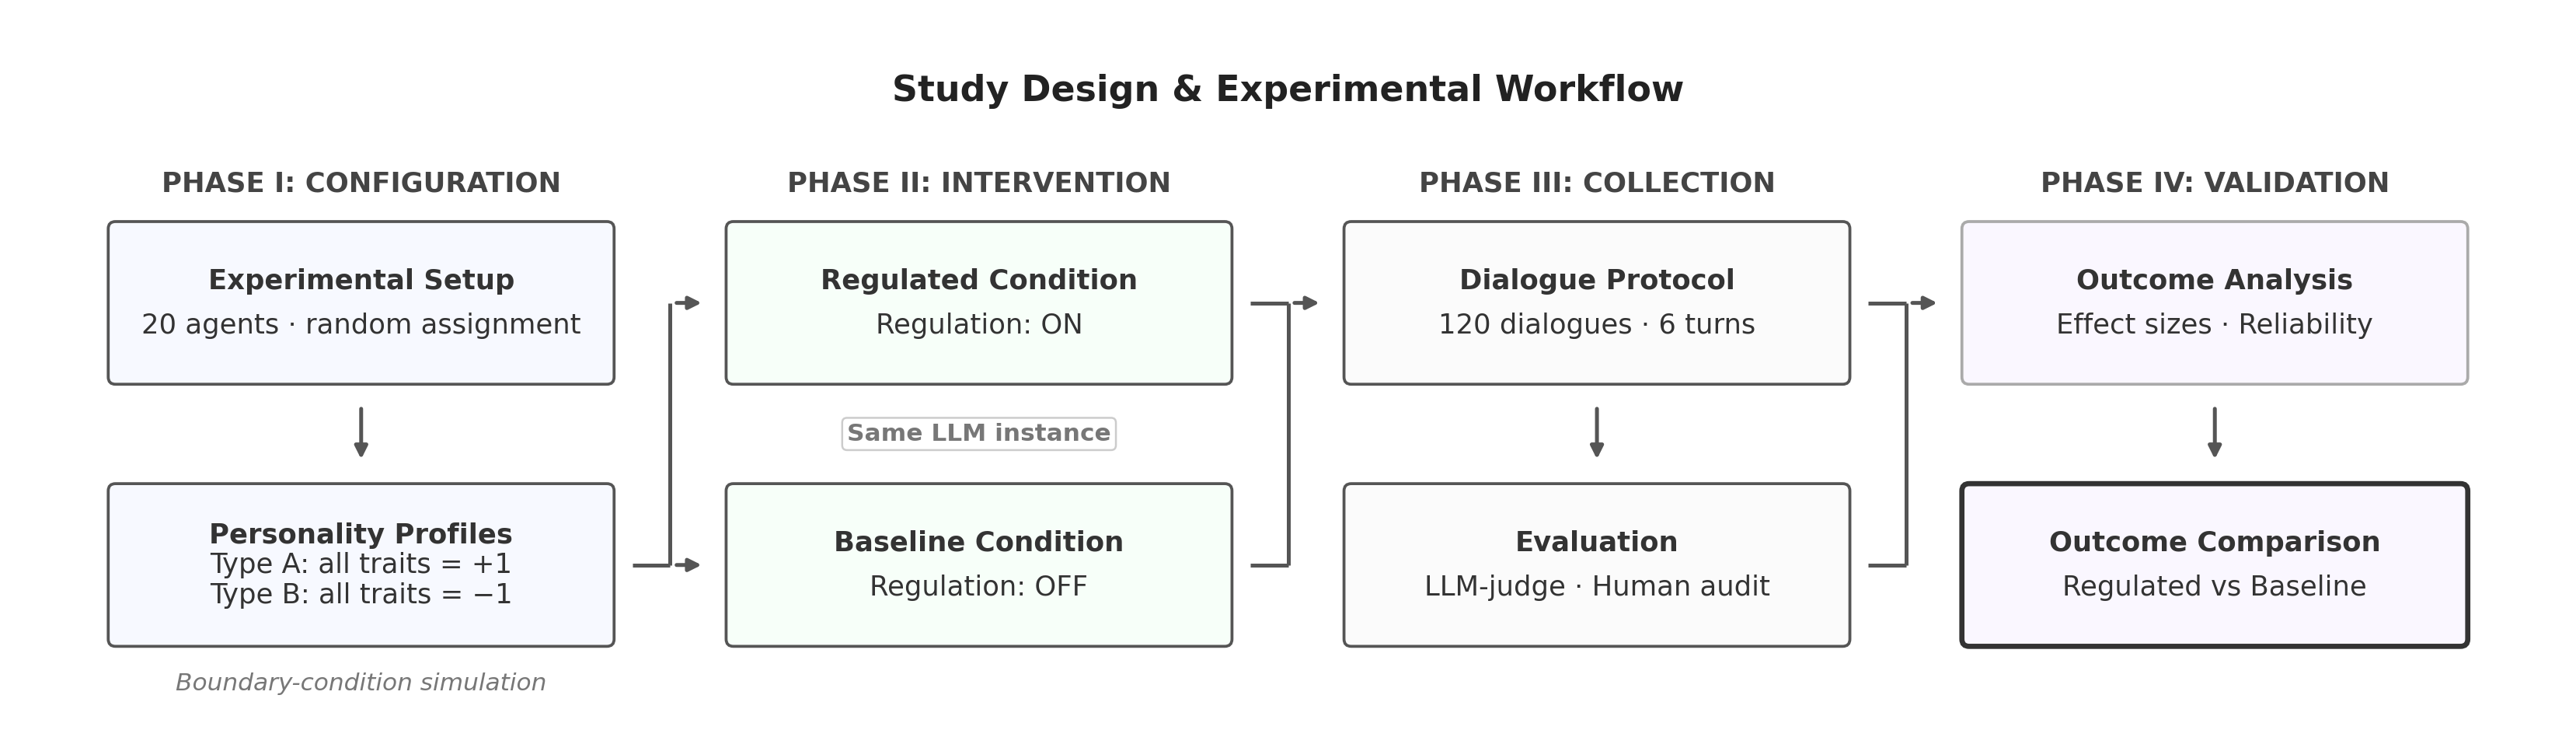
\includegraphics{figures/mdpi/study_design_mdpi.png}
\caption{Study workflow integrating system configuration, dialogue generation, structured LLM-based evaluation (with author-conducted qualitative review), and statistical analysis.}
\label{fig:1}
\end{figure}

\subsubsection{Sample Size Considerations}\label{sample-size-considerations}

The 20 dialogue sessions (5 per cell; 10 per assistant type when aggregated across profiles) represent distinct GPT-4 instantiations with condition-specific system prompts, not human subjects. This sample size was selected for architectural validation purposes based on: (1) a controlled simulation design with limited stochastic variation, (2) computational cost constraints appropriate for proof-of-concept testing, and (3) focus on demonstrating implementation fidelity rather than estimating population-level effects {[}33{]}.

Traditional power analysis is inappropriate because: (1) simulations are controlled and not designed to estimate population-level variability, (2) observed ceiling effects (zero variance) violate power analysis assumptions, and (3) the goal is technical validation, not inferential generalization.

Future human validation will require larger samples (e.g., n $\approx$ 50--100 per condition), in line with clinical trial standards for statistical power, attrition, and inter-individual variability, to capture real-world heterogeneity absent from this simulation {[}34,35,36{]}.

\subsubsection{Ethics and Transparency}\label{ethics-and-transparency}

No human subjects were involved in this study; the user-side prompts/questionnaires were written manually, and the resulting dialogues were generated in a controlled manner using GPT-4-based agents following predefined personality profiles. As the data were synthetic, non-identifiable, and created solely for technical validation, the study fell outside the scope of human-subject research as defined by established ethical frameworks, and formal ethics approval was therefore not required {[}37{]}.

Future studies involving human participants will require full institutional review board approval, comprehensive informed consent addressing AI-based personality profiling and data usage, real-time safety monitoring with clear escalation pathways for psychological distress, and ongoing oversight by qualified mental health professionals {[}38,39{]}. Ethical design of agentic conversational systems should also address questions of interactional respect and user autonomy {[}14{]}.

\subsection{Personality-Adaptive System Architecture}\label{personality-adaptive-system-architecture}

The personality-adaptive system centers on turn-by-turn Big Five detection and regulation over the user model, \textbf{integrated in PROMISE} {[}7{]} through state-attached instructions, storage-backed trait values, and finite-state transitions. Its distinguishing mechanisms are: (i)~\textbf{tri-state personality detection}, with each OCEAN dimension encoded as $\{-1, 0, +1\}$ and an explicit \emph{neutral} state when evidence is insufficient (Table~\ref{tab:1}); (ii)~\textbf{cumulative evidence updating}, so each user turn refines trait estimates from the full dialogue history rather than from isolated utterances; (iii)~\textbf{confidence-threshold triggering}, committing a trait out of neutrality only when detector confidence exceeds $\tau$ (specified in Section~\ref{personality-detection-pipeline}); (iv)~\textbf{parallel per-trait detectors}, i.e., independent LLM-based probes per dimension scored concurrently; and (v)~\textbf{Zurich Model trait-to-behavior mapping}, translating non-neutral traits into stylistic regulation directives along Security, Arousal, and Affiliation before response generation (Section~\ref{theory-driven-regulation}). These mechanisms define the technical contribution evaluated in our simulation; the D--R--E workflow was conceived in prior work {[}68{]} (``a PROMISE-orchestrated pipeline linking per-turn OCEAN detection to Zurich Model-aligned regulation and structured LLM-based evaluation'') and is here extended with a controlled factorial design and systematic statistical outcome analysis.

Within PROMISE, we organize work into Detection (D), Regulation (R), and Evaluation (E) modules for structured operation and quality logging (Figure~\ref{fig:2}); we refer to this three-stage pipeline as the \emph{D--R--E pipeline} throughout the paper. PROMISE supplies model-driven orchestration via hierarchical state-machine modeling. In PROMISE, an interaction is encapsulated as an Agent wrapping a state machine composed of States (with state-specific instruction templates and behaviors) connected by Transitions governed by Decisions (e.g., guards or triggers) and accompanied by Actions (e.g., extraction or summarization). These elements operate over an interaction storage abstraction implemented as a key--value store {[}7{]}. This structure enables explicit state transitions, systematic composition of instructions from modular parts, and transparent logging of decisions and actions across complex interactions.

We embed the core D--R--E pipeline into PROMISE's state-orchestrated architecture as follows:

\begin{itemize}
\item
  \textbf{Detection}: Trait estimation is implemented as a state-driven process that updates a continuous Big Five vector and confidence metrics in the interaction store after each user input. Traits are inferred from linguistic cues in the current interaction context and persist as storage values accessible across states.
\item
  \textbf{Regulation}: Within response-generation states, prompts are augmented with trait-conditioned instructions that softly modulate the assistant's response style---such as tone, pacing, and interpersonal framing---without altering semantic content or task objectives. This is achieved by dynamically composing the base state prompt with trait-aligned augmentation prompts at runtime.
\item
  \textbf{Evaluation}: After each response generation, structured assessment actions execute LLM-based quality checks and log evaluation scores alongside turn identifiers in the interaction store. In the current study, these evaluation outputs are used for offline analysis and do not feed back into detection or regulation during the simulation.
\end{itemize}

This mapping allows the full pipeline to be inspected through PROMISE's explicit state/transition structure and logged decisions/actions, improving reproducibility and auditability of adaptation behavior. The proposed detection--regulation--evaluation logic is conceptually framework-agnostic and could be instantiated in alternative orchestration systems; PROMISE is used here because its declarative state modeling facilitates systematic traceability.

\begin{figure}[H]
\centering
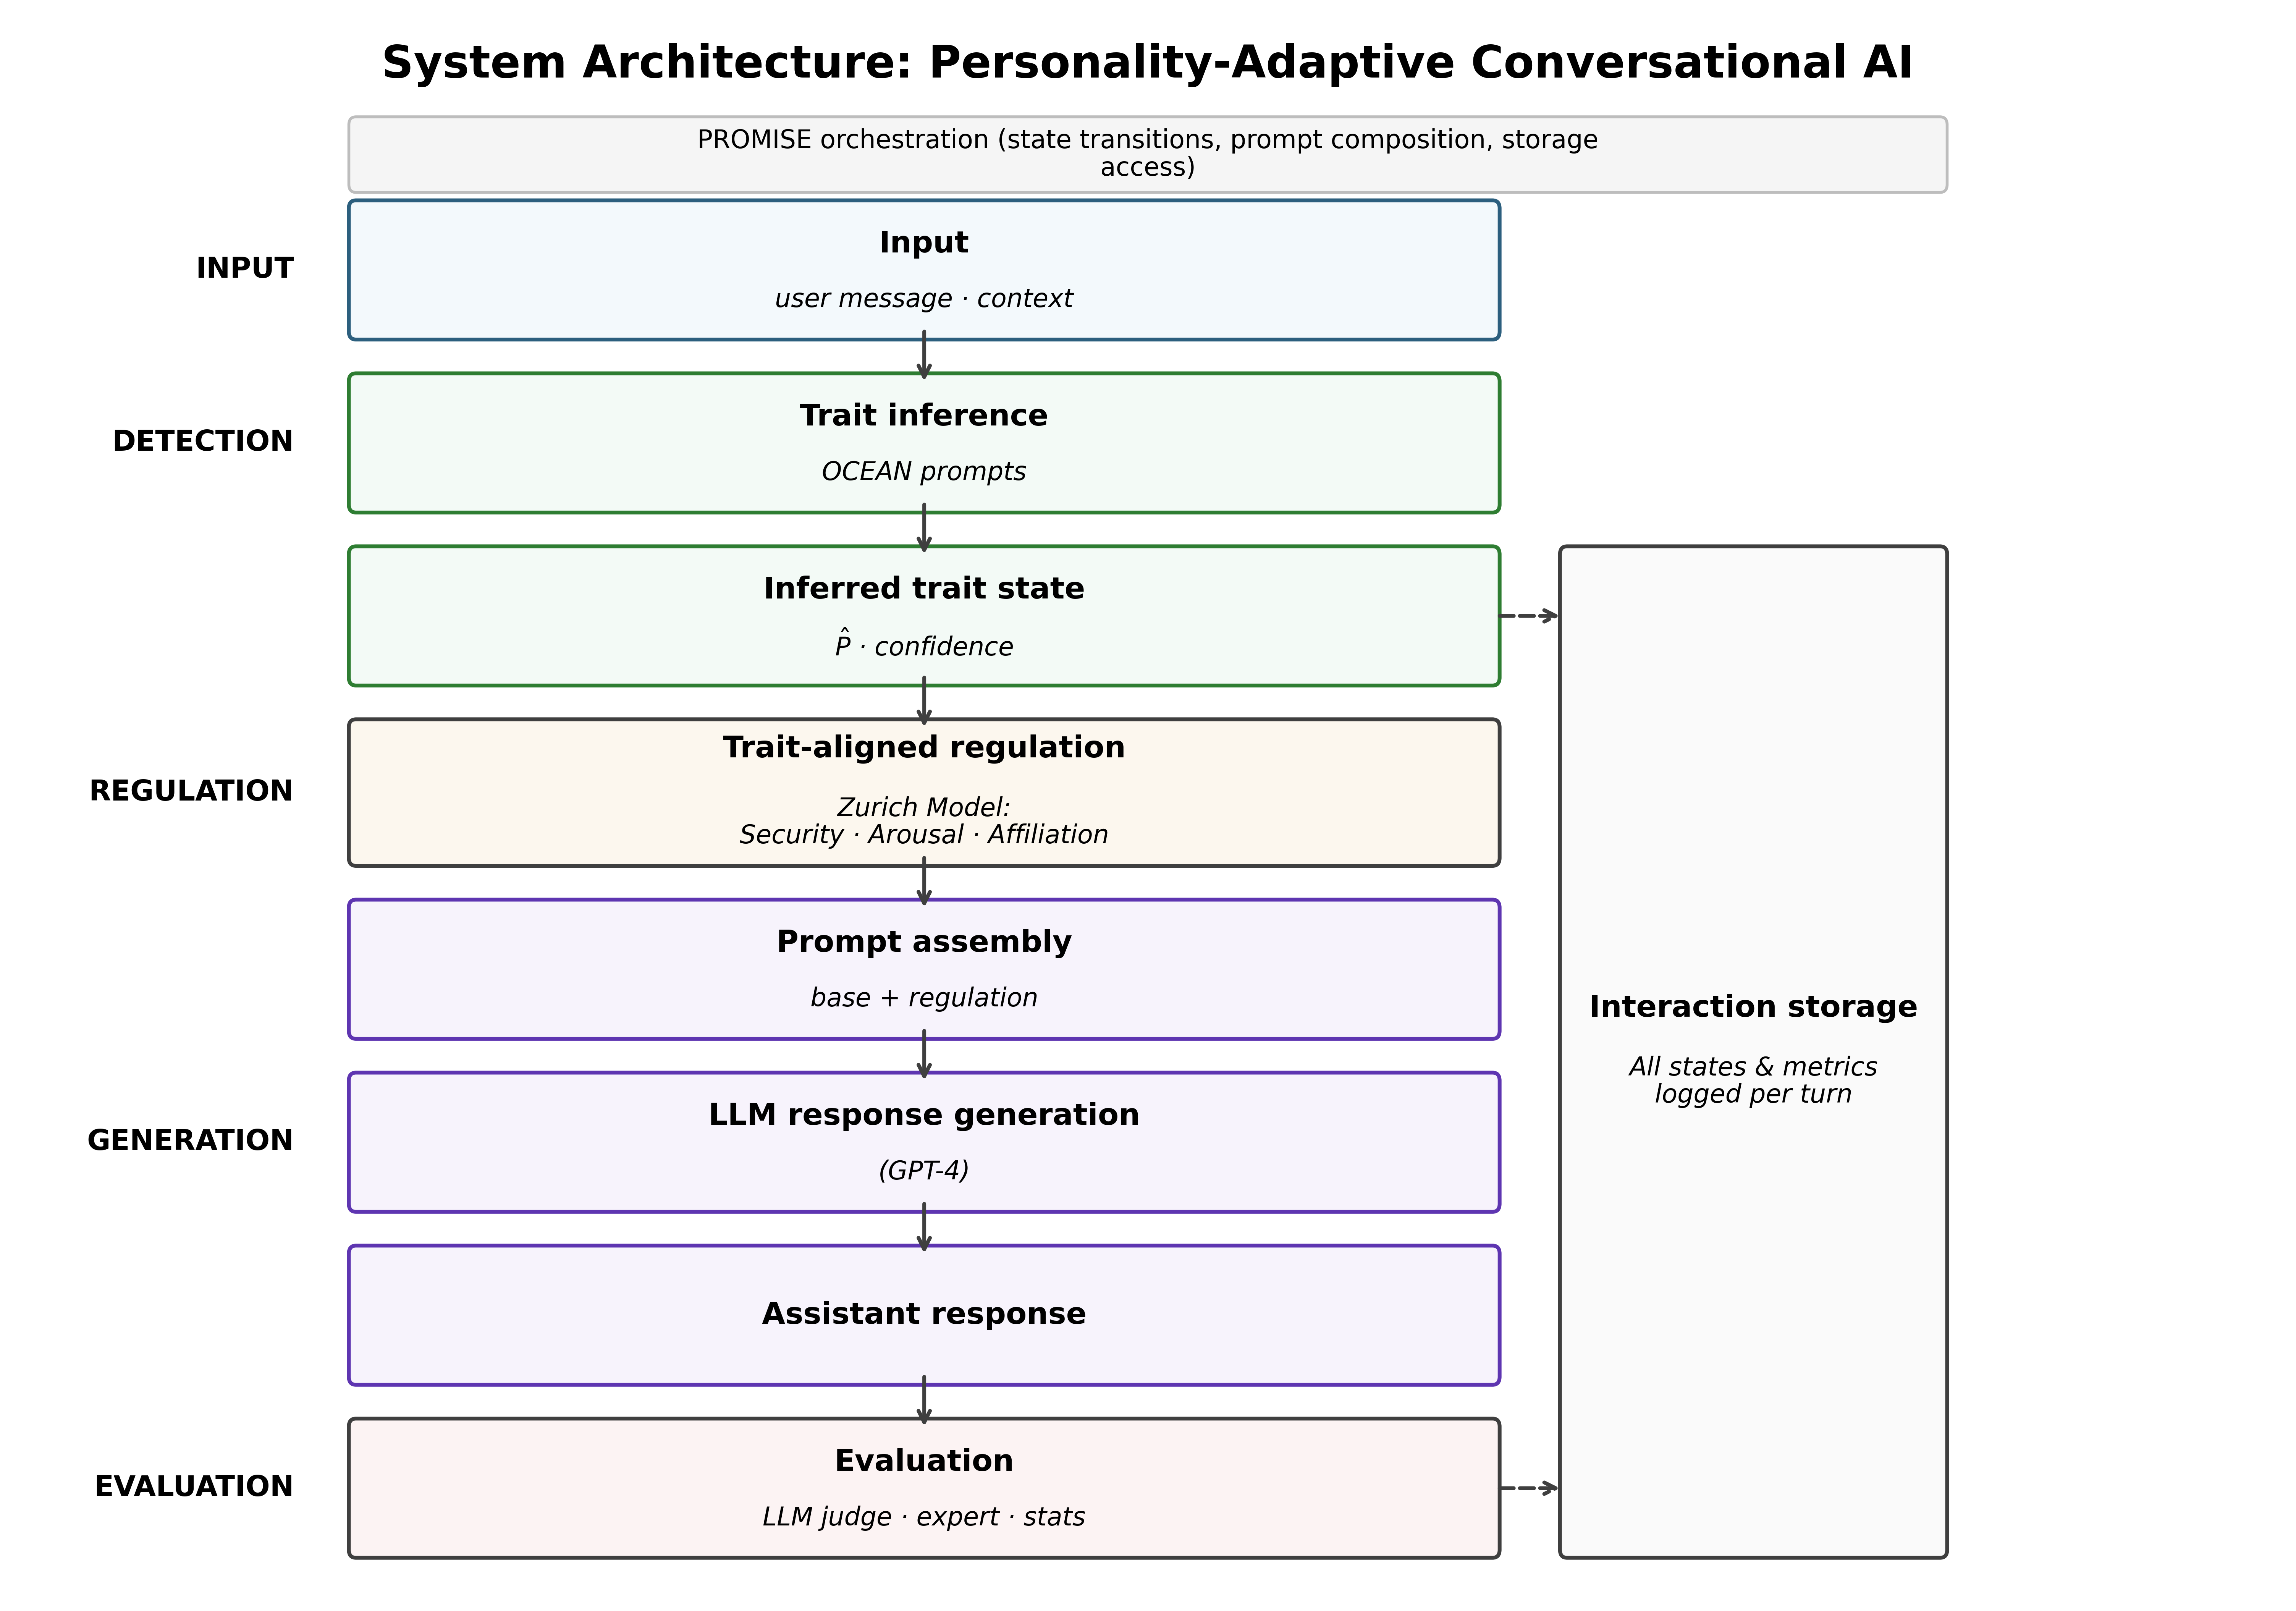
\includegraphics{figures/mdpi/system_architecture_mdpi.png}
\caption{System architecture integrating personality detection (D-module), regulation (R-module), and evaluation (E-module).}
\label{fig:2}
\end{figure}

\subsubsection{Design Principles}\label{design-principles}

The architecture follows three core principles:

\begin{enumerate}
\def\labelenumi{(\roman{enumi})}
\item
  \textbf{Separation of Concerns}: Independent modules with well-defined interfaces enable parallel development and isolated testing. Modules communicate through standardized data structures (JSON) containing personality vectors, regulation instructions, and evaluation scores.
\item
  \textbf{Scalability}: New personality dimensions or regulation strategies can be added without modifying existing components. Trait-to-regulation mapping is externalized as configuration files.
\item
  \textbf{Traceability and Reproducibility}: All detection decisions, regulation instructions, and evaluation scores are logged with timestamps and dialogue turn identifiers. PROMISE's declarative state modeling ensures all behavioral adaptations are traceable to explicit state transitions.
\end{enumerate}

\subsubsection{Data Flow Pipeline}\label{data-flow-pipeline}

The system processes messages through a sequential pipeline (Figure~\ref{fig:3}): (1) User input and dialogue history capture, (2) Personality detection analyzes linguistic cues to infer OCEAN traits, (3) Trait-to-regulation mapping translates personality into behavioral adaptation instructions, (4) Prompt assembly combines regulation with dialogue context, (5) GPT-4 generates personality-adaptive response, (6) Evaluation assesses response quality, and (7) Outputs are logged.

\begin{figure}[H]
\centering
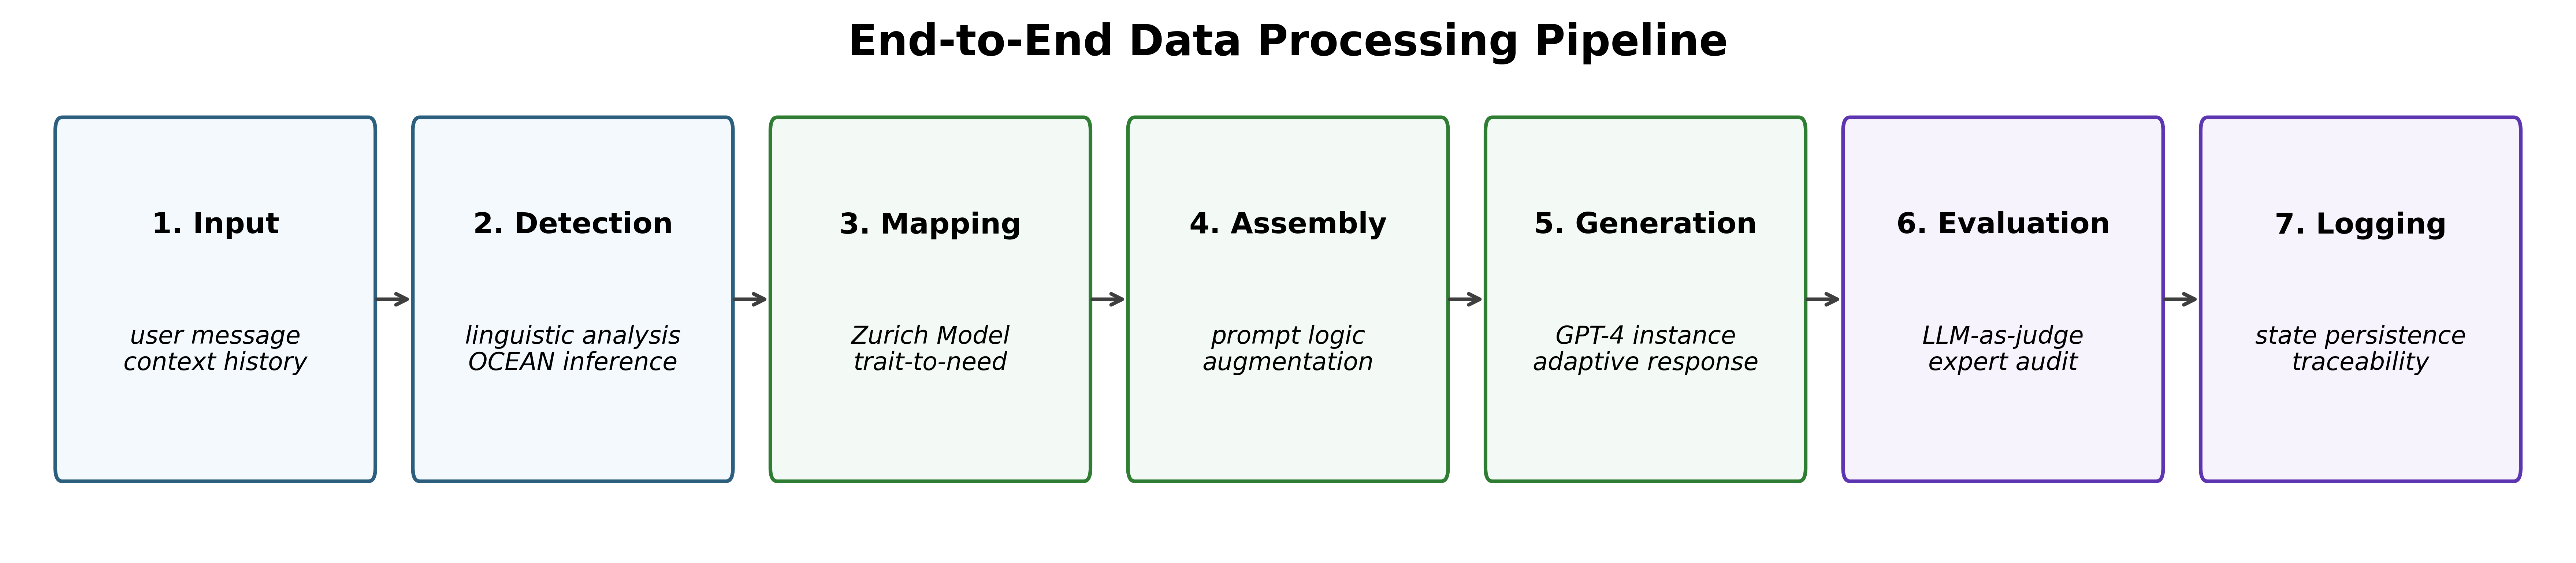
\includegraphics{figures/mdpi/data_flow_mdpi.png}
\caption{End-to-end data flow pipeline.}
\label{fig:3}
\end{figure}

\subsubsection{PROMISE Integration}\label{promise-integration}

PROMISE operationalizes complex interactions by composing prompts from modular parts attached to states and transitions {[}7{]}. In typical PROMISE execution, transition decisions (trigger/guard) are evaluated against the accumulated state utterances before generating the next assistant response; if no transition fires, the assistant response is generated from a composed prompt that includes the state prompt and the dialogue history. PROMISE also supports nested state machines (``outer states'') that maintain an aggregated utterance history across inner states and can inject shared role prompts into all contained states, enabling consistent behavior across multi-stage interactions. Additionally, PROMISE supports placeholder-based instruction templates filled at runtime and actions that extract structured outputs into interaction storage (key--value store), which can be reused by downstream states and system components {[}7{]}. Our integration leverages these mechanisms to (i) persist the current Big Five vector and confidence in storage, (ii) compose trait-aligned regulation instructions into the response-generation prompt, and (iii) log evaluation outputs with turn identifiers for traceability.

\subsection{System Implementation}\label{system-implementation}

This section describes how the system implements (i) real-time personality detection and (ii) theory-driven regulation, both orchestrated within PROMISE (Section~\ref{personality-adaptive-system-architecture}).

\subsubsection{Personality Detection Pipeline}\label{personality-detection-pipeline}

We represent the user's Big Five profile as a five-dimensional vector (P = (O, C, E, A, N)), with each trait ($\in \{-1, 0, +1\}$) {[}3,9,41{]}. In this simulation, the personality vector functions as a predefined reference target for controlled evaluation rather than psychometric ground truth; detection accuracy denotes agreement with the pre-specified simulated profile.

\begin{longtable}[]{@{}
  >{\raggedright\arraybackslash}p{(\linewidth - 4\tabcolsep) * \real{0.2500}}
  >{\raggedright\arraybackslash}p{(\linewidth - 4\tabcolsep) * \real{0.3929}}
  >{\raggedright\arraybackslash}p{(\linewidth - 4\tabcolsep) * \real{0.3571}}@{}}
\caption{Big Five personality trait operationalization. Neuroticism is inverse-coded: +1 denotes emotional stability (low neuroticism), and -1 denotes emotional vulnerability (high neuroticism).}\label{tab:1}\\
\toprule\noalign{}
\begin{minipage}[b]{\linewidth}\raggedright
Trait
\end{minipage} & \begin{minipage}[b]{\linewidth}\raggedright
+1 (High)
\end{minipage} & \begin{minipage}[b]{\linewidth}\raggedright
-1 (Low)
\end{minipage} \\
\midrule\noalign{}
\endhead
\bottomrule\noalign{}
\endlastfoot
Openness & Curious, imaginative, open to novelty & Prefers routine, resistant to new ideas \\
Conscientiousness & Organized, disciplined, structured & Disorganized, impulsive, spontaneous \\
Extraversion & Outgoing, energetic, assertive & Reserved, quiet, withdrawn \\
Agreeableness & Cooperative, empathetic, friendly & Critical, skeptical, confrontational \\
Neuroticism* & Calm, emotionally stable, resilient & Anxious, emotionally sensitive, insecure \\
\end{longtable}

After each user input, the system updates (P) using cumulative evidence across dialogue history, following a belief-updating logic similar to Bayesian belief updating {[}43{]}. PROMISE orchestrates this pipeline via hierarchical state machines, parallel trait detectors, and explicit transition logic (Section~\ref{personality-adaptive-system-architecture}). Inference produces trait values (-1/0/+1) and confidence scores, with trait state transitions triggered when confidence exceeds $\tau$ = 0.7 (Figure~\ref{fig:4}).

\begin{figure}[H]
\centering
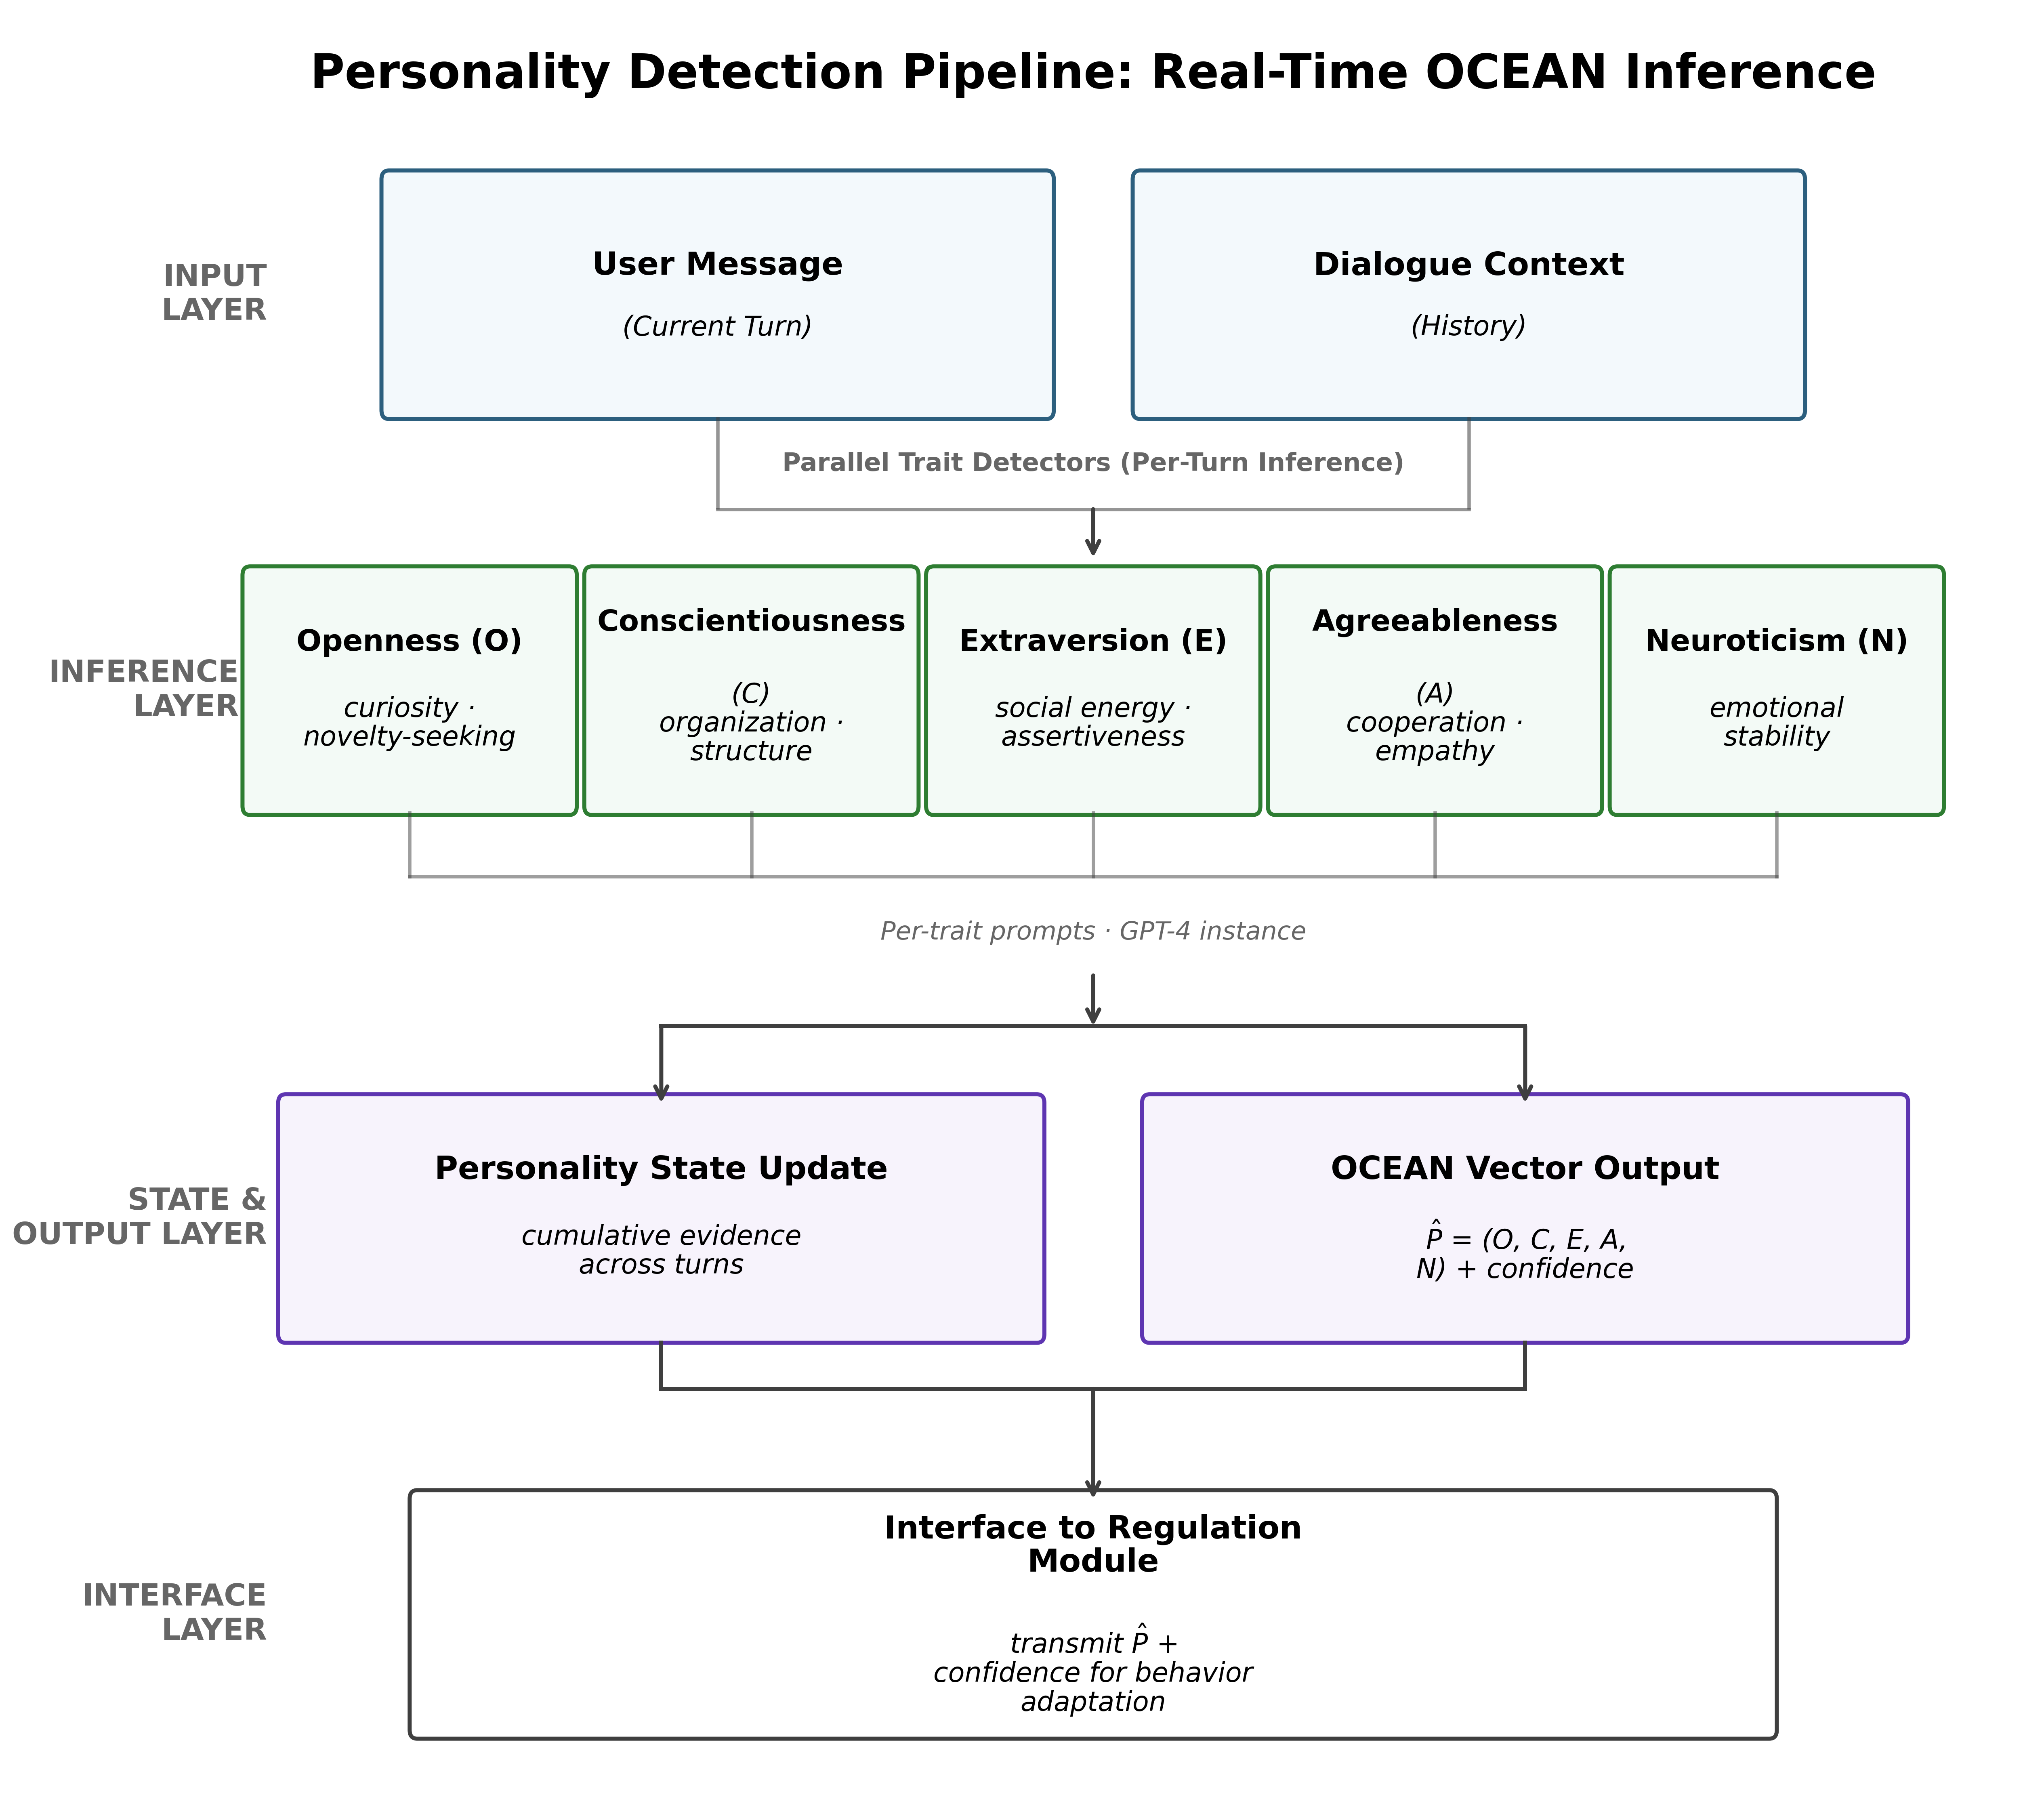
\includegraphics{figures/mdpi/detection_pipeline_mdpi.png}
\caption{Personality detection pipeline implementing turn-by-turn Big Five inference.}
\label{fig:4}
\end{figure}

The detection component is implemented as a modular service integrated into PROMISE. It uses GPT-4 (gpt-4-0613) with trait-specific prompts grounded in personality psychology {[}44--50{]}. The pipeline executes the following stages: (1) message processing, (2) prompt assembly, (3) parallel LLM inference across traits, (4) response parsing and confidence assessment, (5) state update, and (6) downstream transmission to the regulation module.

Average processing time was 2.3 ± 0.8 seconds per turn (measured across 120 turns), with parallel trait detection reducing latency by \textasciitilde60\% versus sequential processing.

\subsubsection{Theory-Driven Regulation}\label{theory-driven-regulation}

Regulation translates detected traits into behavioral adaptations grounded in the Zurich Model of Social Motivation {[}10,26--29{]}, which links personality to three motivational domains: Security, Arousal, and Affiliation (Section~\ref{from-affective-computing-to-personality-aware-digital-support}). Table~\ref{tab:2} and Figure~\ref{fig:5} present the mapping from Big Five traits to motivational domains and corresponding behavioral adjustment strategies.

\begin{figure}[H]
\centering
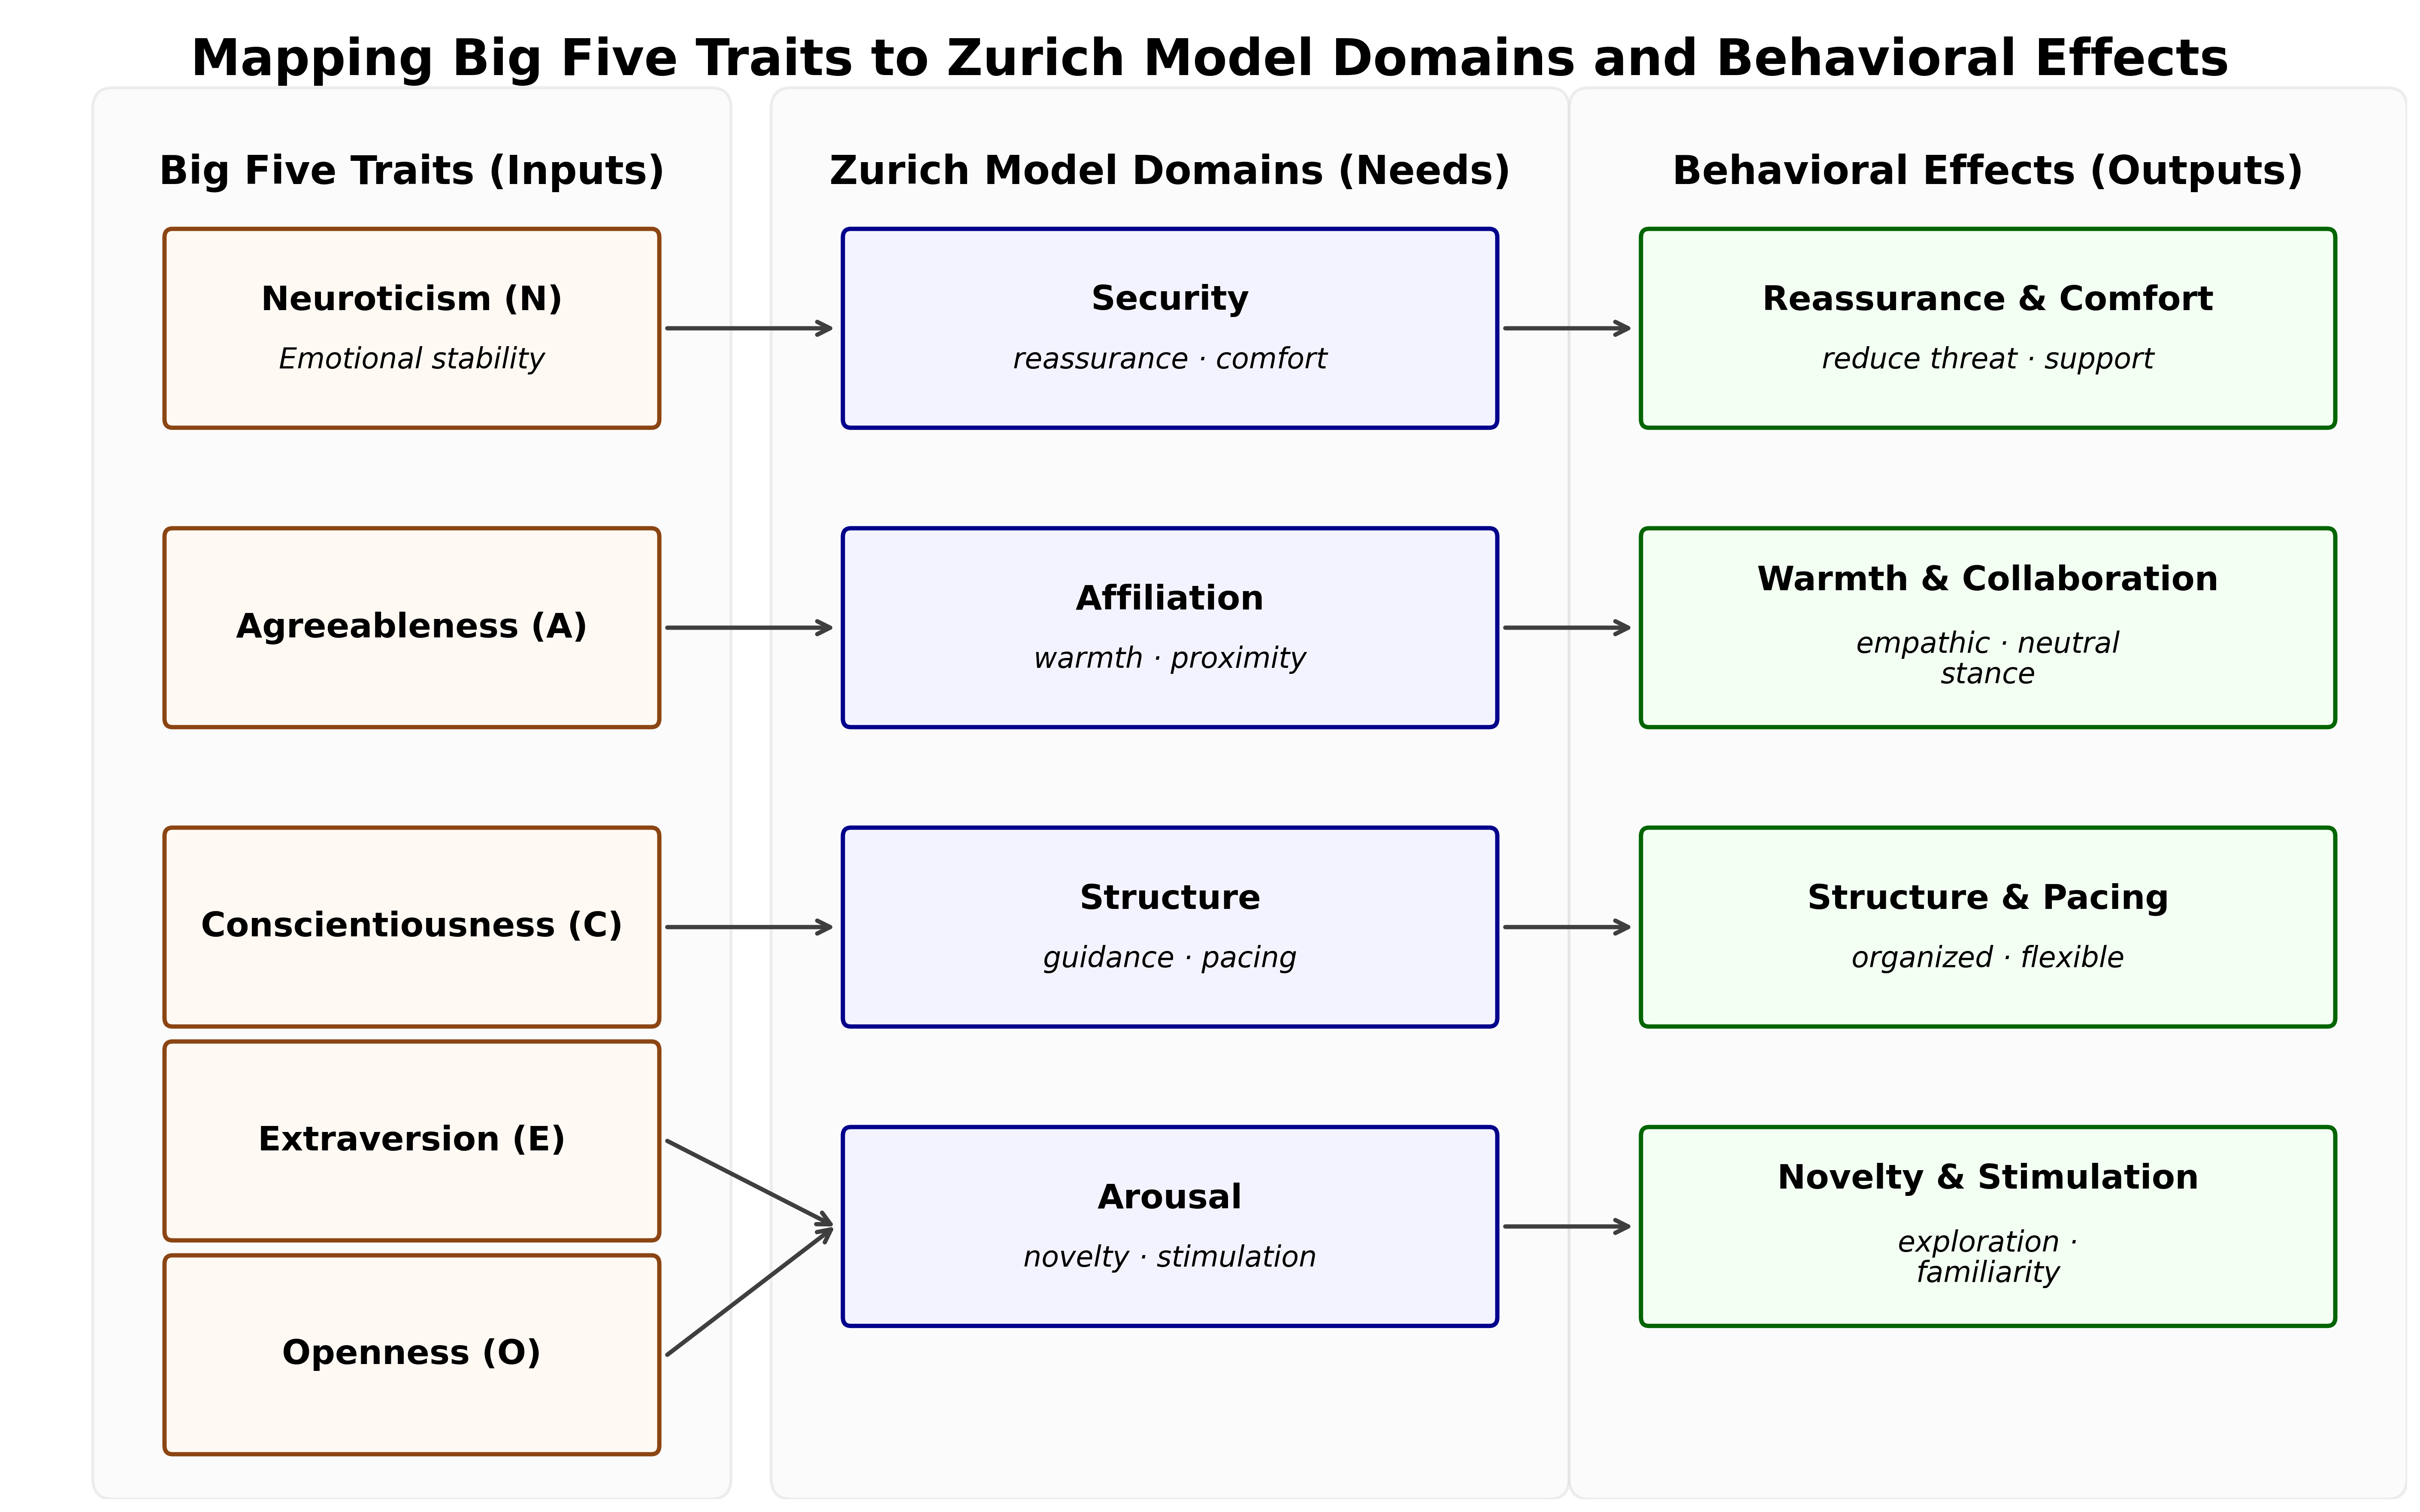
\includegraphics{figures/mdpi/trait_mapping_mdpi.png}
\caption{Mapping from Big Five traits to motivational domains to conversational behavior effects.}
\label{fig:5}
\end{figure}

\begin{longtable}[]{@{}
  >{\raggedright\arraybackslash}p{(\linewidth - 6\tabcolsep) * \real{0.1300}}
  >{\raggedright\arraybackslash}p{(\linewidth - 6\tabcolsep) * \real{0.2600}}
  >{\raggedright\arraybackslash}p{(\linewidth - 6\tabcolsep) * \real{0.3100}}
  >{\raggedright\arraybackslash}p{(\linewidth - 6\tabcolsep) * \real{0.3000}}@{}}
\caption{Behavioral adjustment strategies mapped by Zurich Model motivational domain. Conscientiousness modulates interaction structure independently of the three core domains.}\label{tab:2}\\
\toprule\noalign{}
\begin{minipage}[b]{\linewidth}\raggedright
Domain
\end{minipage} & \begin{minipage}[b]{\linewidth}\raggedright
Trait
\end{minipage} & \begin{minipage}[b]{\linewidth}\raggedright
+1 (High)
\end{minipage} & \begin{minipage}[b]{\linewidth}\raggedright
-1 (Low)
\end{minipage} \\
\midrule\noalign{}
\endhead
\bottomrule\noalign{}
\endlastfoot
Security & Neuroticism (N) & Reassure stability and confidence & Offer extra comfort; acknowledge anxieties \\
Arousal & Openness (O) & Invite exploration and novelty & Focus on familiar topics; reduce novelty \\
Arousal & Extraversion (E) & Energetic, sociable tone & Calm, low-key style with reflective space \\
Affiliation & Agreeableness (A) & Warmth, empathy, collaboration & Neutral, matter-of-fact stance \\
Cross-cutting & Conscientiousness (C) & Provide organized, structured guidance & Flexible, relaxed, spontaneous demeanor \\
\end{longtable}

After each personality update, PROMISE composes an integrated regulation instruction by concatenating trait-relevant behavior prompts for all non-neutral traits (Figure~\ref{fig:6}). When trait recommendations conflict, the system prioritizes emotional safety (Security domain) over stimulation (Arousal domain), consistent with clinical guidance {[}51{]}.

\begin{figure}[H]
\centering
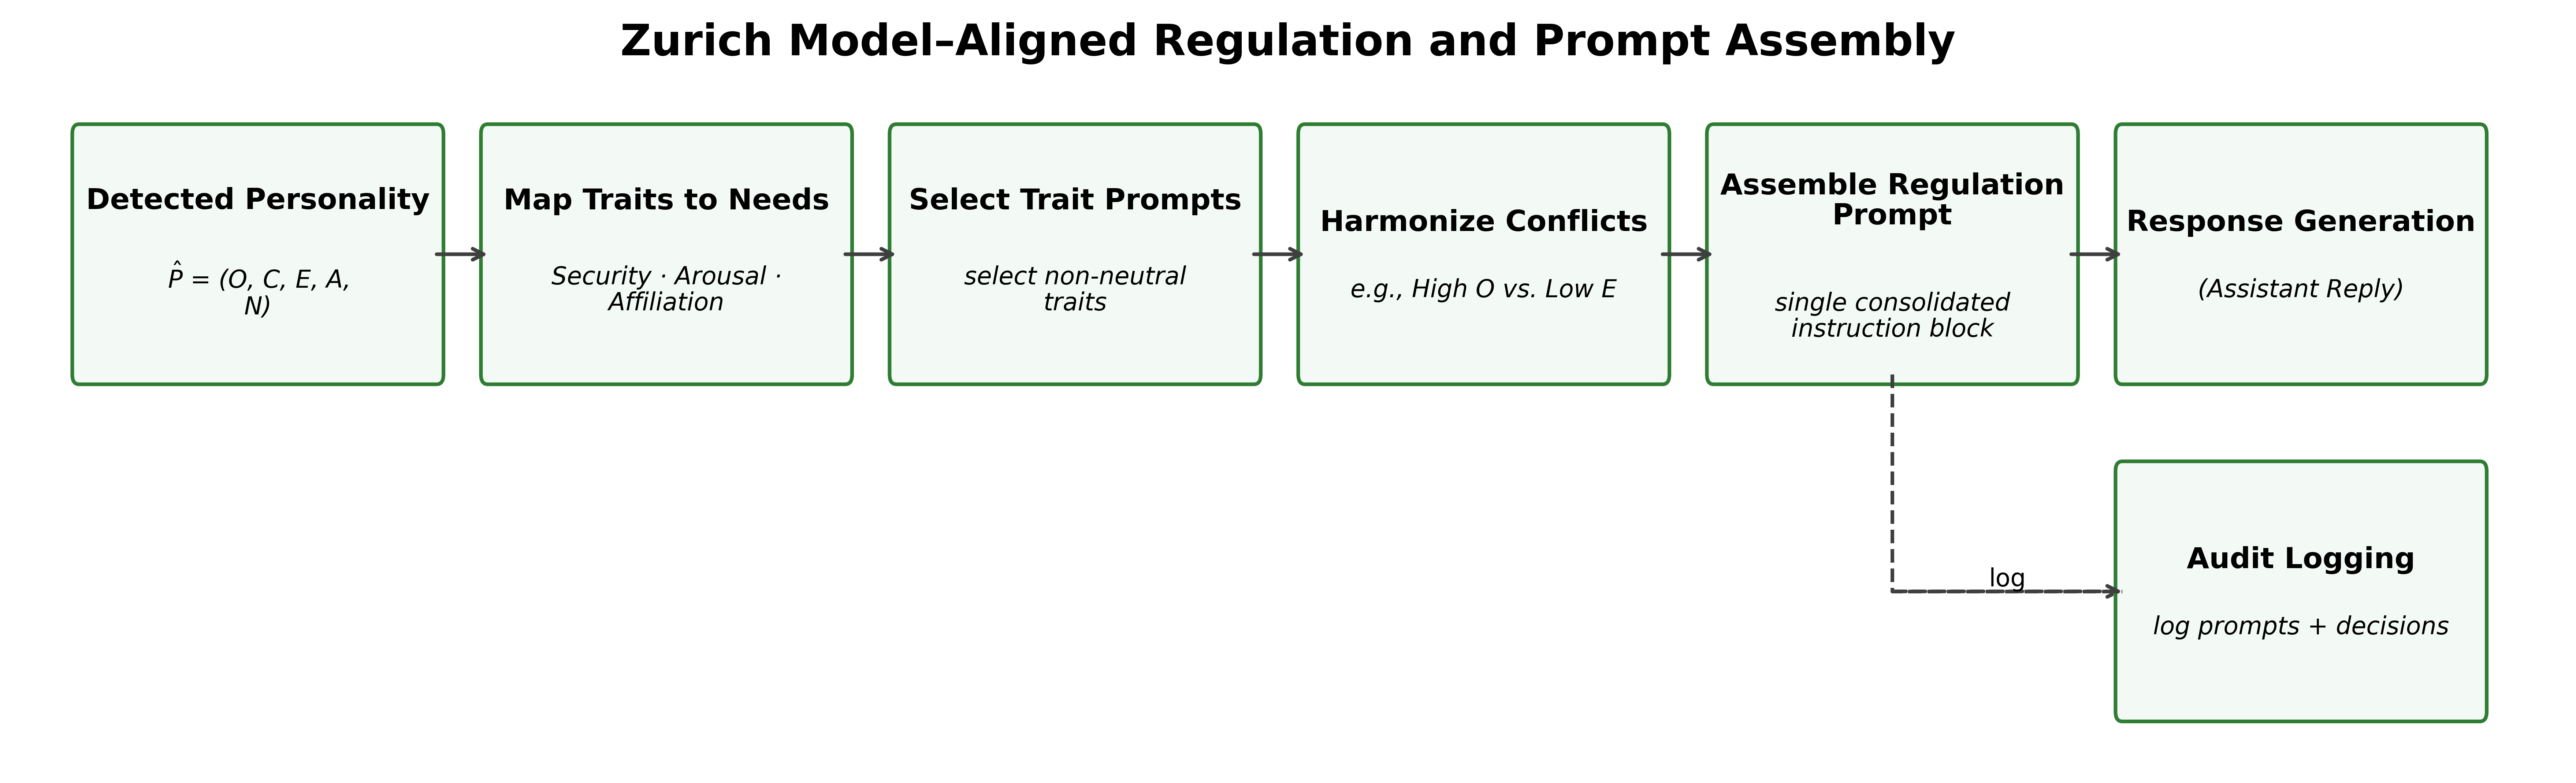
\includegraphics{figures/mdpi/regulation_workflow_mdpi.png}
\caption{Regulation workflow: after each personality update, PROMISE concatenates trait-relevant behavior prompts for all non-neutral traits and assembles an integrated regulation instruction, prioritizing the Security domain over Arousal in cases of conflict.}
\label{fig:6}
\end{figure}

\subsection{Experimental Materials and Procedure}\label{experimental-materials-and-procedure}

\subsubsection{Personality Profile Simulation}\label{personality-profile-simulation}

We implemented two boundary-condition personality profiles representing extremes of human personality variation {[}40,42,53{]}. Type A (all traits: $+1, +1, +1, +1, +1$) embodied extreme positive trait levels. Type B (all traits: $-1, -1, -1, -1, -1$) embodied opposite extremes.

These extreme configurations were deliberately selected to maximize signal for detection and regulation mechanisms. While not representative of typical distributions {[}3{]}, such profiles offer superior diagnostic value for validating this implementation before testing with moderate profiles {[}53{]}.

Detection and regulation performance are evaluated against these synthetic reference profiles as ground truth within the simulation environment. Profiles were encoded into GPT-4 system prompts consistently exhibiting target trait levels across turns.

\subsubsection{Agent Configuration}\label{agent-configuration}

Twenty dialogue sessions (assistant-condition instantiations) were generated across four $2 \times 2$ cells: Regulated--Type~A ($n=5$), Regulated--Type~B ($n=5$), Baseline--Type~A ($n=5$), Baseline--Type~B ($n=5$). Regulated assistants received system prompts incorporating dynamic detection modules and trait-aligned regulation instructions, with inferences updating per-turn. Baseline assistants received static supportive response prompts without personality-specific adaptation. Each assistant instantiation used a separate GPT-4 call configuration (model: gpt-4-0613, temperature=0.7, max\_tokens=500). GPT-4 (gpt-4-0613) was selected because it represented the state-of-the-art instruction-following model at the time of data collection (June--August 2024) and provided the balance of controllability, context length, and response quality required by the PROMISE orchestration framework. The core architectural findings---that explicit regulation instructions produce consistent personality-need fulfillment whereas non-adaptive prompting does not---are expected to generalize to successor models (e.g., GPT-4o, GPT-4-turbo); if anything, stronger base models may yield higher detection accuracy and more nuanced regulation, though independent validation with those models remains necessary.

\subsubsection{Dialogue Structure and Data Collection}\label{dialogue-structure-and-data-collection}

For each personality type (A and B), we generated 5 regulated and 5 baseline dialogue sessions. Each session consisted of 6 user--assistant exchanges (i.e., 6 assistant responses paired with 6 user messages), resulting in 120 assistant turns total across the full design (2 profiles $\times$ 2 assistant types $\times$ 5 sessions $\times$ 6 assistant turns). All conversations followed a standardized six-exchange structure balancing sufficient interaction depth for valid personality detection with manageable evaluation complexity.

Each session followed a consistent scenario progression across the six exchanges (opening support offer $\rightarrow$ initial disclosure $\rightarrow$ elaboration $\rightarrow$ reframing $\rightarrow$ coping/next-step guidance $\rightarrow$ closing), with user messages generated to reflect the target personality profile and assistants responding either with regulated (personality-adaptive) or baseline (non-adaptive) strategies.

User messages were generated by separate GPT-4 instances (model: gpt-4-0613) instantiated with personality profile prompts ensuring consistent trait expression. Conversations were exported into structured Evaluation Matrices (Excel format). Data collection occurred over 4 weeks (June--July 2024). The simulation data were generated during the initial system development phase, prior to the present study {[}68{]}.

\subsection{Evaluation Procedure}\label{evaluation-procedure}

\subsubsection{Evaluation Criteria and Scoring Framework}\label{evaluation-criteria-and-scoring-framework}

The evaluation measured effectiveness of personality-regulated assistant interactions versus baselines using a structured Evaluation Matrix and a dedicated Evaluator GPT, with each assistant output scored on detection accuracy, regulation effectiveness, emotional tone, relevance, and fulfillment of personality-specific emotional needs. The evaluator methodology was conceived in prior work {[}68{]} (``a dedicated GPT-4 evaluator instance scoring regulated turns across five criteria and baseline turns across three criteria on a trinary Yes/Not-Sure/No scale, assessed row-by-row with full dialogue context and personality profile''). Regulated assistants were evaluated across five criteria: Detection Accuracy, Regulation Effectiveness, Emotional Tone Appropriate, Relevance \& Coherence, and Personality Needs Addressed.

Baseline assistants were assessed on three criteria only (Emotional Tone, Relevance \& Coherence, Personality Needs), as detection and regulation were not implemented. All criteria used a trinary scoring scale (\textit{Yes} = 2, \textit{Not Sure} = 1, \textit{No} = 0) {[}54{]}. Figure~\ref{fig:7} illustrates the full evaluation framework and scoring pipeline.

\begin{figure}[H]
\centering
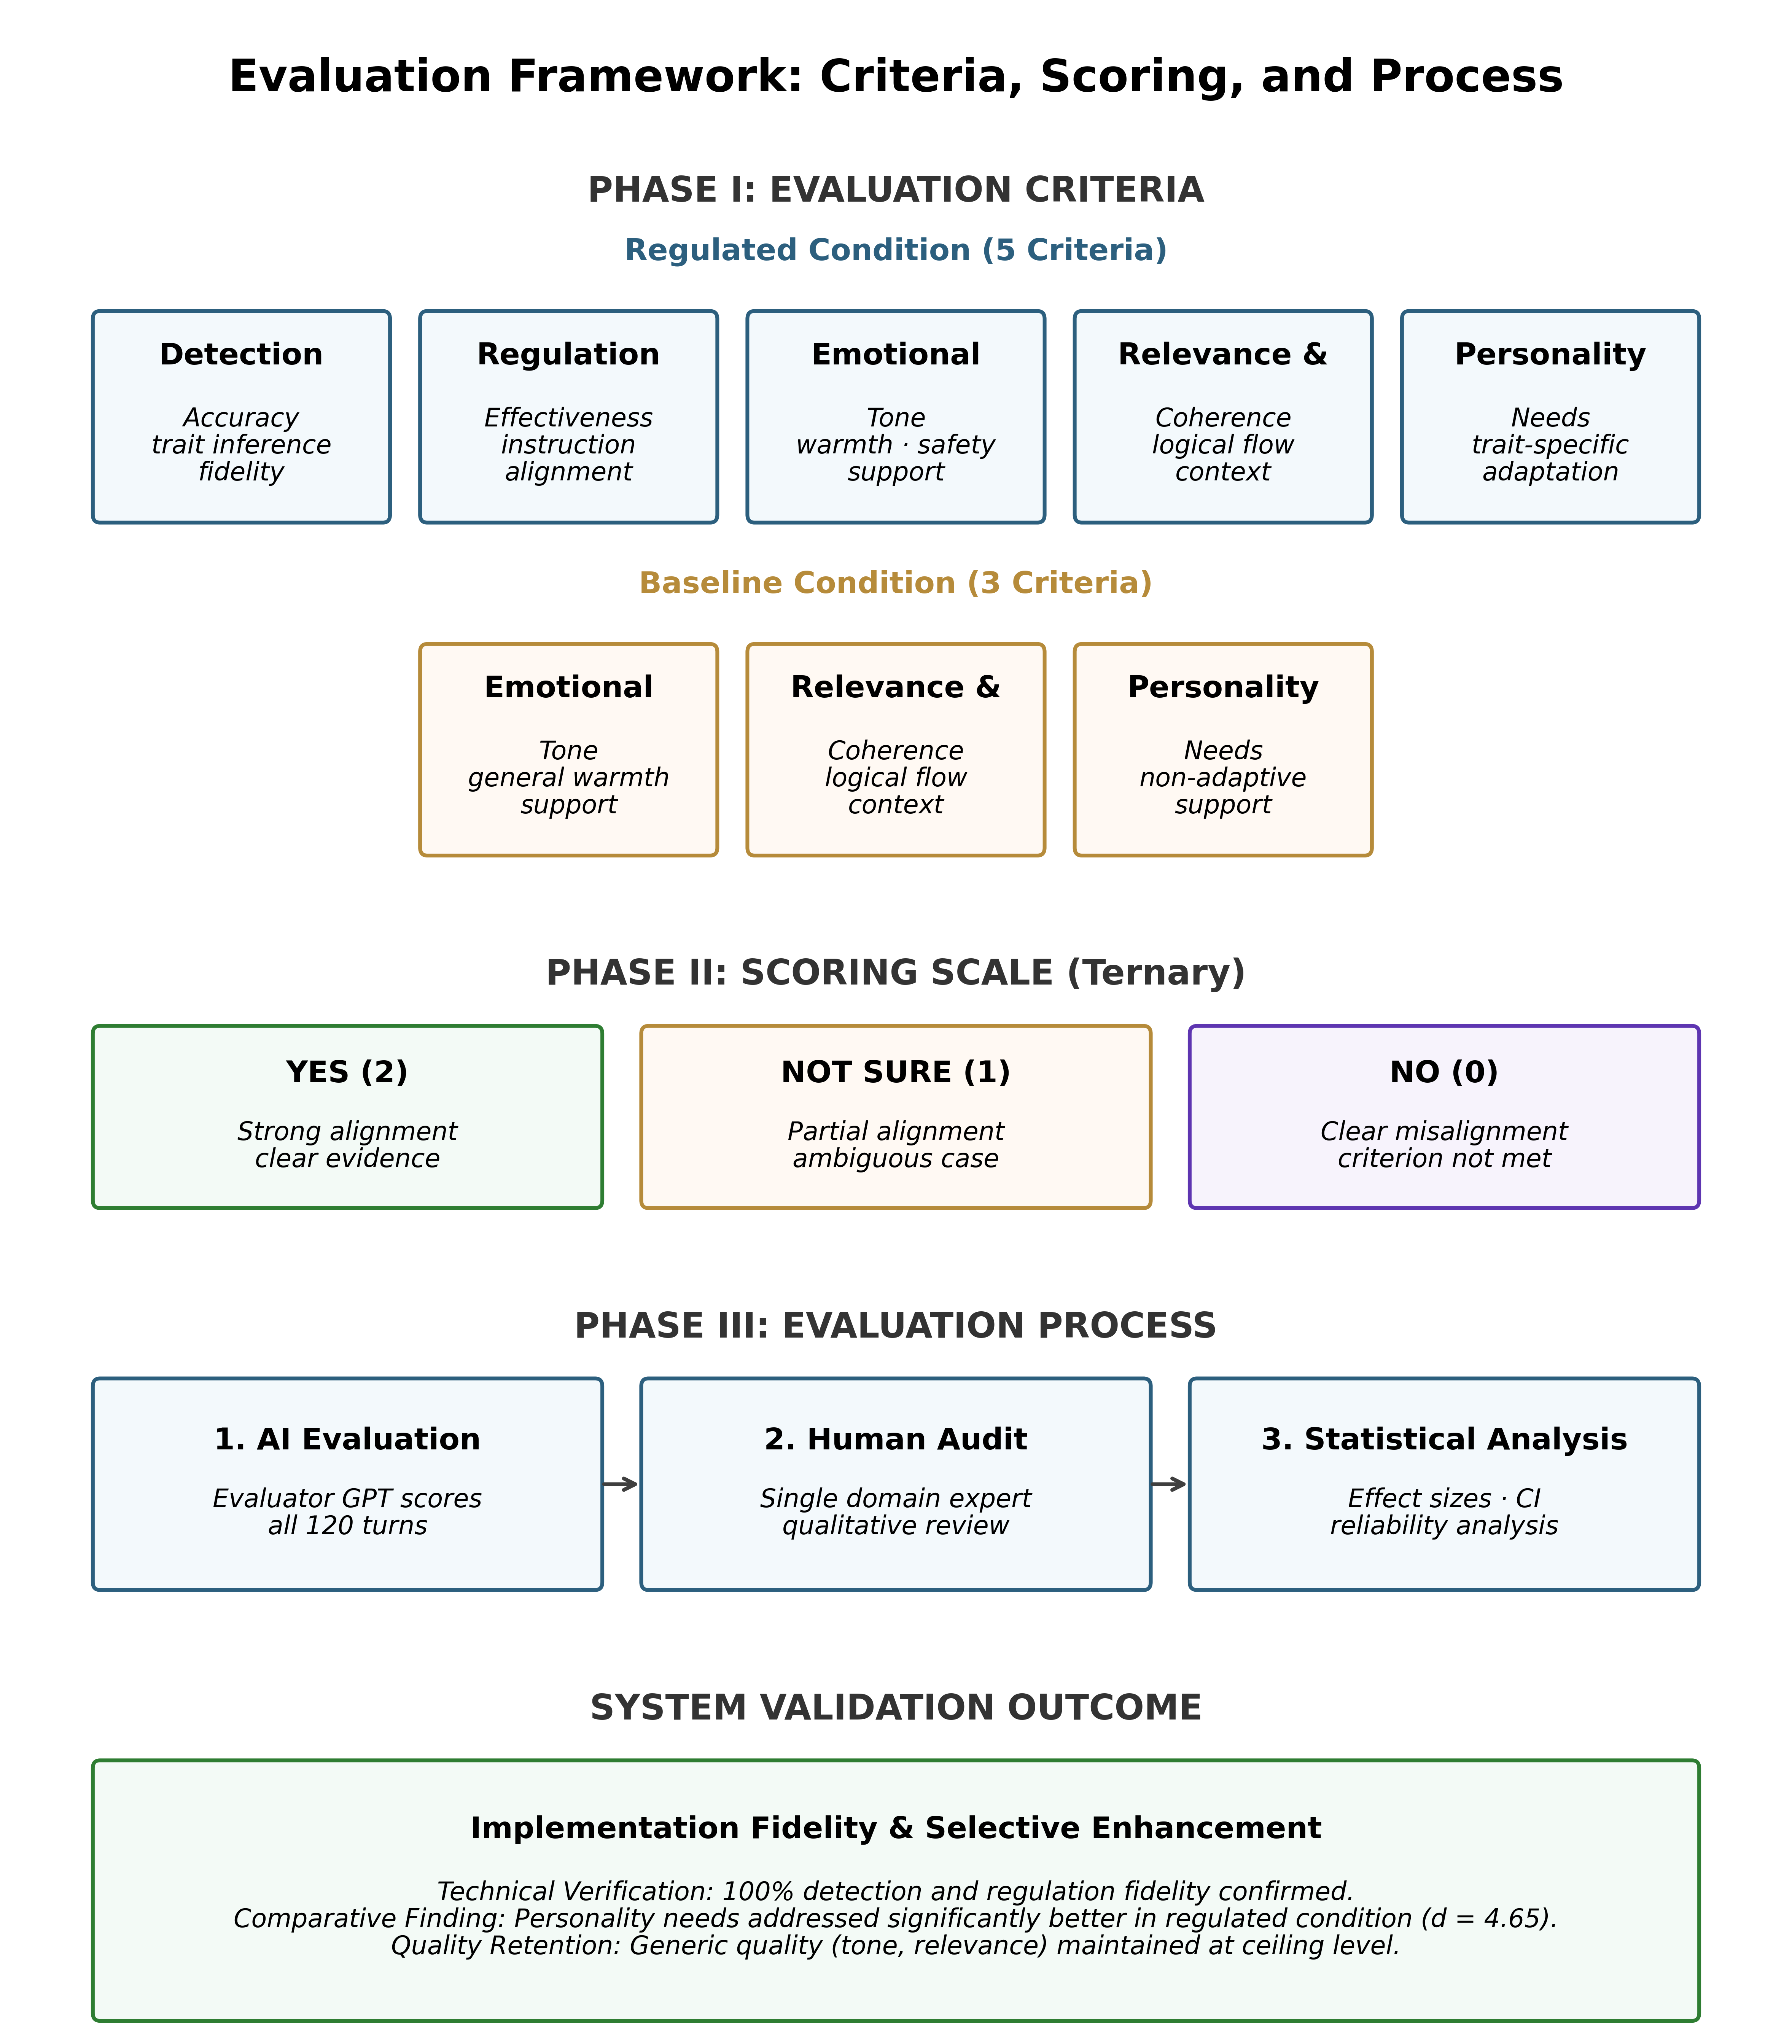
\includegraphics{figures/mdpi/evaluation_framework_mdpi.png}
\caption{Evaluation framework and scoring pipeline.}
\label{fig:7}
\end{figure}

\subsubsection{LLM-Based Evaluator System}\label{llm-based-evaluator-system}

A specialized Evaluator GPT-4 instance was developed using custom-designed prompts for each criterion, following the ``LLM-as-judge'' paradigm {[}55,56{]}. The evaluator assessed responses objectively by analyzing conversations one row at a time. Measures to mitigate evaluator bias: evaluations conducted separately for regulated and baseline assistants; comprehensive context provided including full dialogue history and personality profile; evaluator informed that detection accuracy improves incrementally; temperature set to 0.3 to reduce stochastic variation.

\subsubsection{Evaluation Validity and Author-Led Qualitative Review}\label{evaluation-validity-and-author-validation}

To address ``AI-evaluating-AI'' concerns, two contributing authors (Samuel Devdas and Jiahua Duojie) reviewed all evaluation matrices and provided qualitative commentary for each rated item. Their assessments largely aligned with the agent-generated detections and criterion judgements across the regulated conversations, with one instance marked as uncertain. These author notes provide an internal audit trail supporting the face validity and plausibility of automated ratings; they do \emph{not} constitute impartial verification by independent external raters.

As quantitative ratings are LLM-generated and qualitative validation was performed by study authors, the results should be interpreted as proof-of-concept evidence under controlled simulation conditions, with attendant risk of confirmation bias. This design offers interpretive support rather than quantitative inter-rater reliability or third-party expert certification. Establishing full evaluation credibility requires: (i) at least two independent human raters scoring an overlapping subset of turns to quantify inter-rater reliability (e.g., Krippendorff's $\alpha$ {[}11{]}), and (ii) human--AI agreement analysis for automated scoring (e.g., Cohen's $\kappa$ {[}57,58{]}).

\subsection{Analysis and Reproducibility}\label{analysis-and-reproducibility}

\subsubsection{Primary and Secondary Outcomes}\label{primary-and-secondary-outcomes}

The primary outcome was ``Personality Needs Addressed,'' measured on a trinary scale (\textit{Yes} = 2, \textit{Not Sure} = 1, \textit{No} = 0). Secondary outcomes included Detection Accuracy, Regulation Effectiveness, Emotional Tone Appropriateness, and Relevance \& Coherence. Ratings were applied at the assistant-turn level (10 dialogue sessions per condition $\times$ 6 assistant turns = 60 outputs per condition), yielding 60 observations per metric {[}59{]}.

\subsubsection{Statistical Analysis}\label{statistical-analysis}

Between-group differences were evaluated using two-tailed independent samples \textit{t}-tests for normally distributed metrics and Mann-Whitney U tests for non-normally distributed metrics (normality assessed via Shapiro-Wilk tests, $\alpha$ = 0.05). Effect sizes were calculated using Cohen's d with pooled standard deviation and interpreted using conventional thresholds (small d = 0.2, medium d = 0.5, large d = 0.8) {[}60{]}. For the primary outcome, we also report Cliff's \(\delta\) (probability that a randomly chosen regulated score exceeds a randomly chosen baseline score, rescaled to \([-1,1]\)) as a distribution-free complement when conditions show heavy separation on a discrete scale. Confidence intervals (95\%) were calculated using bias-corrected bootstrap (10,000 iterations) {[}61{]}. Statistical significance was set at $\alpha$ = 0.05. All inferential statistics are reported for comparability with prior conversational AI studies and should not be interpreted as evidence of population-level effects {[}62{]}.

\subsubsection{Reproducibility and Computational Environment}\label{reproducibility-and-computational-environment}

All statistical analyses were conducted in Python 3.9+ using scipy (v1.9.0) for statistical tests, numpy (v1.23.0) for effect size calculations, and matplotlib/seaborn for visualizations. Experiments used GPT-4 API (model: gpt-4-0613, OpenAI Python SDK v1.3.5) with temperature = 0.7 for agent responses and temperature = 0.3 for evaluator responses. All random operations used fixed seed (Python: 42).

Complete implementation code, system prompts, experimental protocols, and conversation transcripts are available at GitHub: \url{https://github.com/SamuelDevdas/socialbehaviourregulation-SD}. The repository includes detection module source code (Java 21), regulation prompt templates (JSON), evaluator GPT system prompts (Markdown), complete conversation transcripts (anonymized CSV, 120 turns), statistical analysis scripts (Python/Jupyter notebooks), and Docker configuration files.

Important limitation: GPT-4 API responses exhibit stochastic variation even at temperature = 0 due to probabilistic sampling {[}63{]}. In this study, the fixed random seed (42) and locked model snapshot (gpt-4-0613) are expected to substantially reduce run-to-run variation, though full determinism cannot be guaranteed by design.

\section{Results}\label{results}

\subsection{Overview of Results}\label{overview-of-results}

This section reports (i) dataset distribution, (ii) technical detection/regulation performance, and (iii) comparative effectiveness of regulated versus baseline assistants, followed by qualitative examples illustrating the observed adaptation pattern.

\subsection{Data Quality and Sample Distribution}\label{data-quality-and-sample-distribution}

The evaluation dataset comprised 10 matched conversation pairs across two extreme personality profiles: Type A (OCEAN: +1, +1, +1, +1, +1) and Type B (OCEAN: -1, -1, -1, -1, -1), with 5 conversations per profile. Each conversation contained 6 user--assistant exchanges, yielding 60 rated assistant turns per condition (regulated: n = 60; baseline: n = 60).

Figure~\ref{fig:8} provides a comprehensive overview of sample characteristics and data quality, including sample sizes across conditions (Panel A), the distribution of personality profiles (Panel B), the $2 \times 2$ experimental design (Panel C), and data completeness across evaluation metrics (Panel D). All metrics exceeded the 95\% completeness threshold, with no systematic missingness patterns between conditions. Detection and Regulation metrics apply only to the regulated condition.

\begin{figure}[!t]
\centering
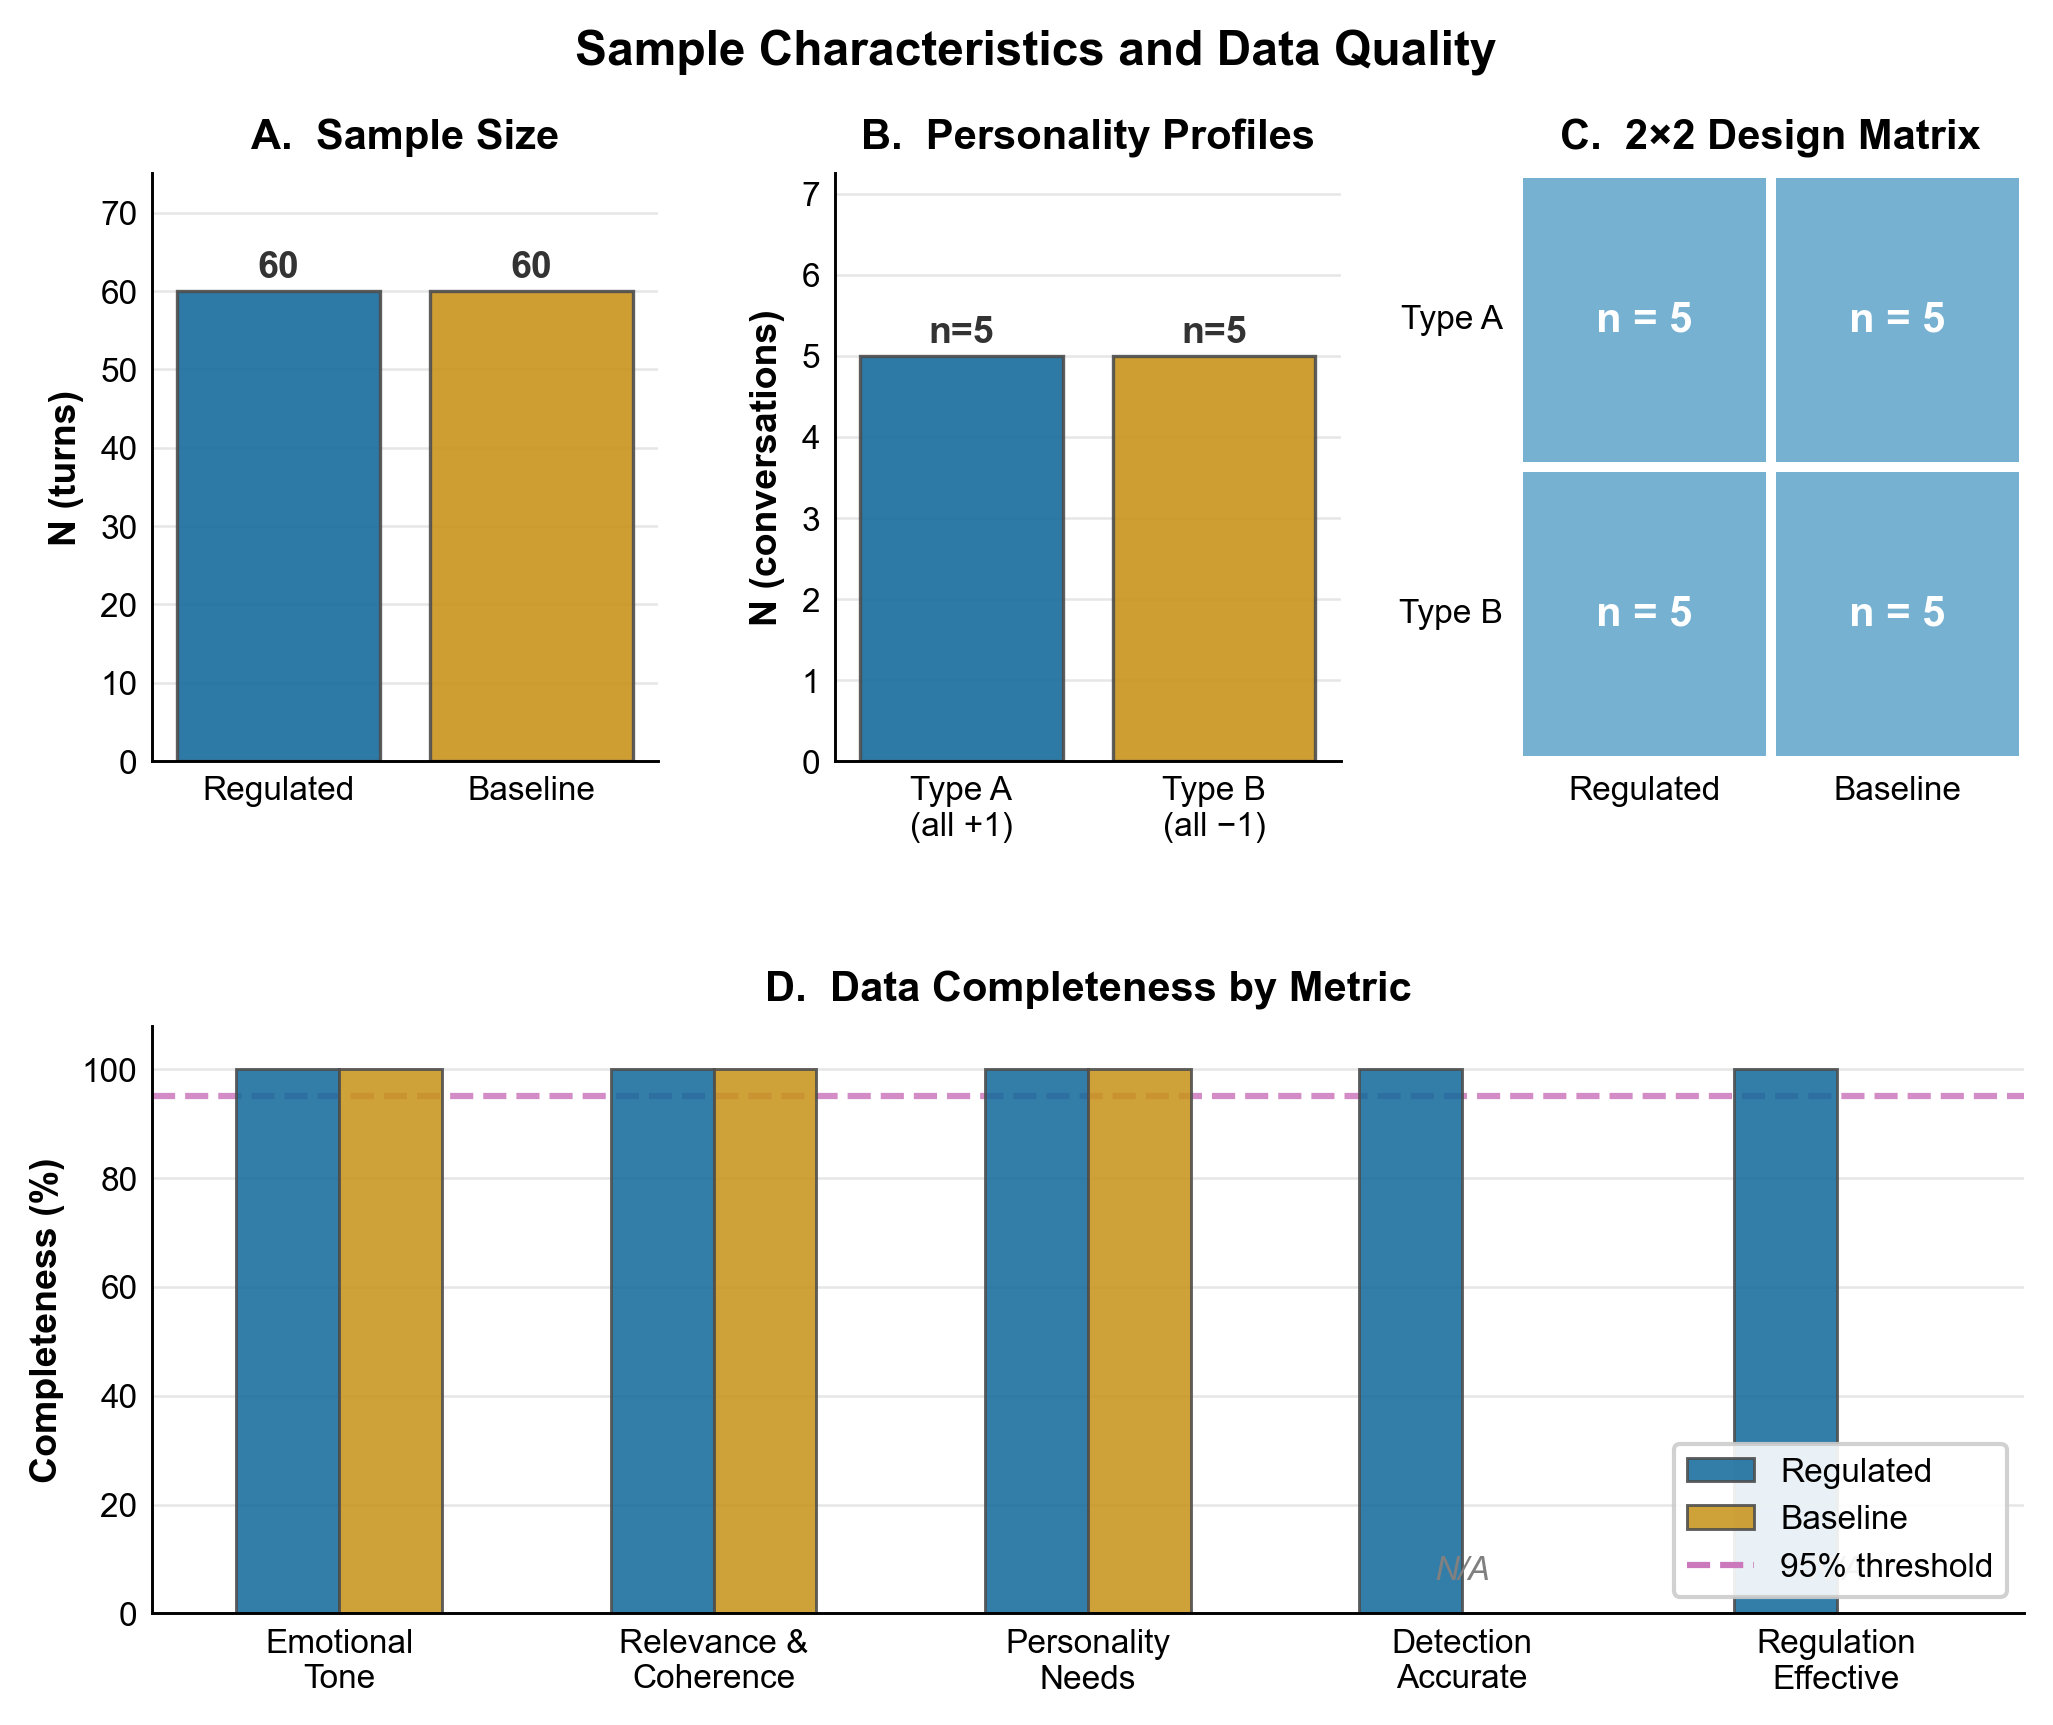
\includegraphics{figures/04_sample_quality.png}
\caption{Sample characteristics and data quality summary. (A) Distribution of assistant turns analyzed; (B) Personality profiles representing experimental arms; (C) \(2 \times 2\) factorial design matrix showing balanced group sizes; (D) Data completeness percentage by metric and condition. All metrics meet or exceed rigorous standards for valid statistical comparison.}
\label{fig:8}
\end{figure}

The balanced $2 \times 2$ design (5 conversations $\times$ 2 profiles $\times$ 2 conditions) and near-complete data support valid between-group comparisons. The small sample size (n = 10 conversations) provides adequate power for detecting large effects (d \textgreater{} 0.8) expected under controlled simulation conditions.

\subsection{Detection and Regulation Performance}\label{detection-and-regulation-performance}

Regulated agents achieved near-perfect performance on core technical requirements.

\textbf{Table 3.} Detection and Regulation Performance Summary

Detection accuracy reached 98.3\% (59/60 \emph{Yes}, 1/60 \emph{Not sure}) for extreme simulated profiles, with regulation effectiveness achieving 100\% (60/60 successful implementations). These results confirm the system reliably executes the designed detection and regulation logic when tested with these profiles.

Near-perfect technical performance establishes that the system can identify personality patterns and adjust behavior accordingly in the vast majority of cases. The critical question becomes whether this technical capability produces actual improvements in conversational quality.

\subsubsection{Personality Vector Consistency}\label{personality-vector-consistency}

Figures~\ref{fig:9} and~\ref{fig:10} provide diagnostic evidence of detected personality vector patterns across turns. Analysis of 60 detected personality vectors (one per regulated conversation turn) revealed dimension-specific detection fidelity: Extraversion, Agreeableness (Type A), and Neuroticism showed near-perfect alignment with intended profiles ($\geq$87\% correct), while Conscientiousness and Agreeableness (Type B) exhibited more frequent Mid (0) detections, reflecting the detector's use of a neutral state ($0$) when conversational evidence for extreme trait expression was insufficient. Most conversations showed within-conversation stability; limited within-conversation variation was observed in a small number of sessions (e.g., Extraversion in conversation A-5, Openness in B-5 (where A/B denotes the personality profile type)), consistent with the cumulative-evidence updating mechanism described in Section~\ref{personality-detection-pipeline}.

\begin{figure}[H]
\centering
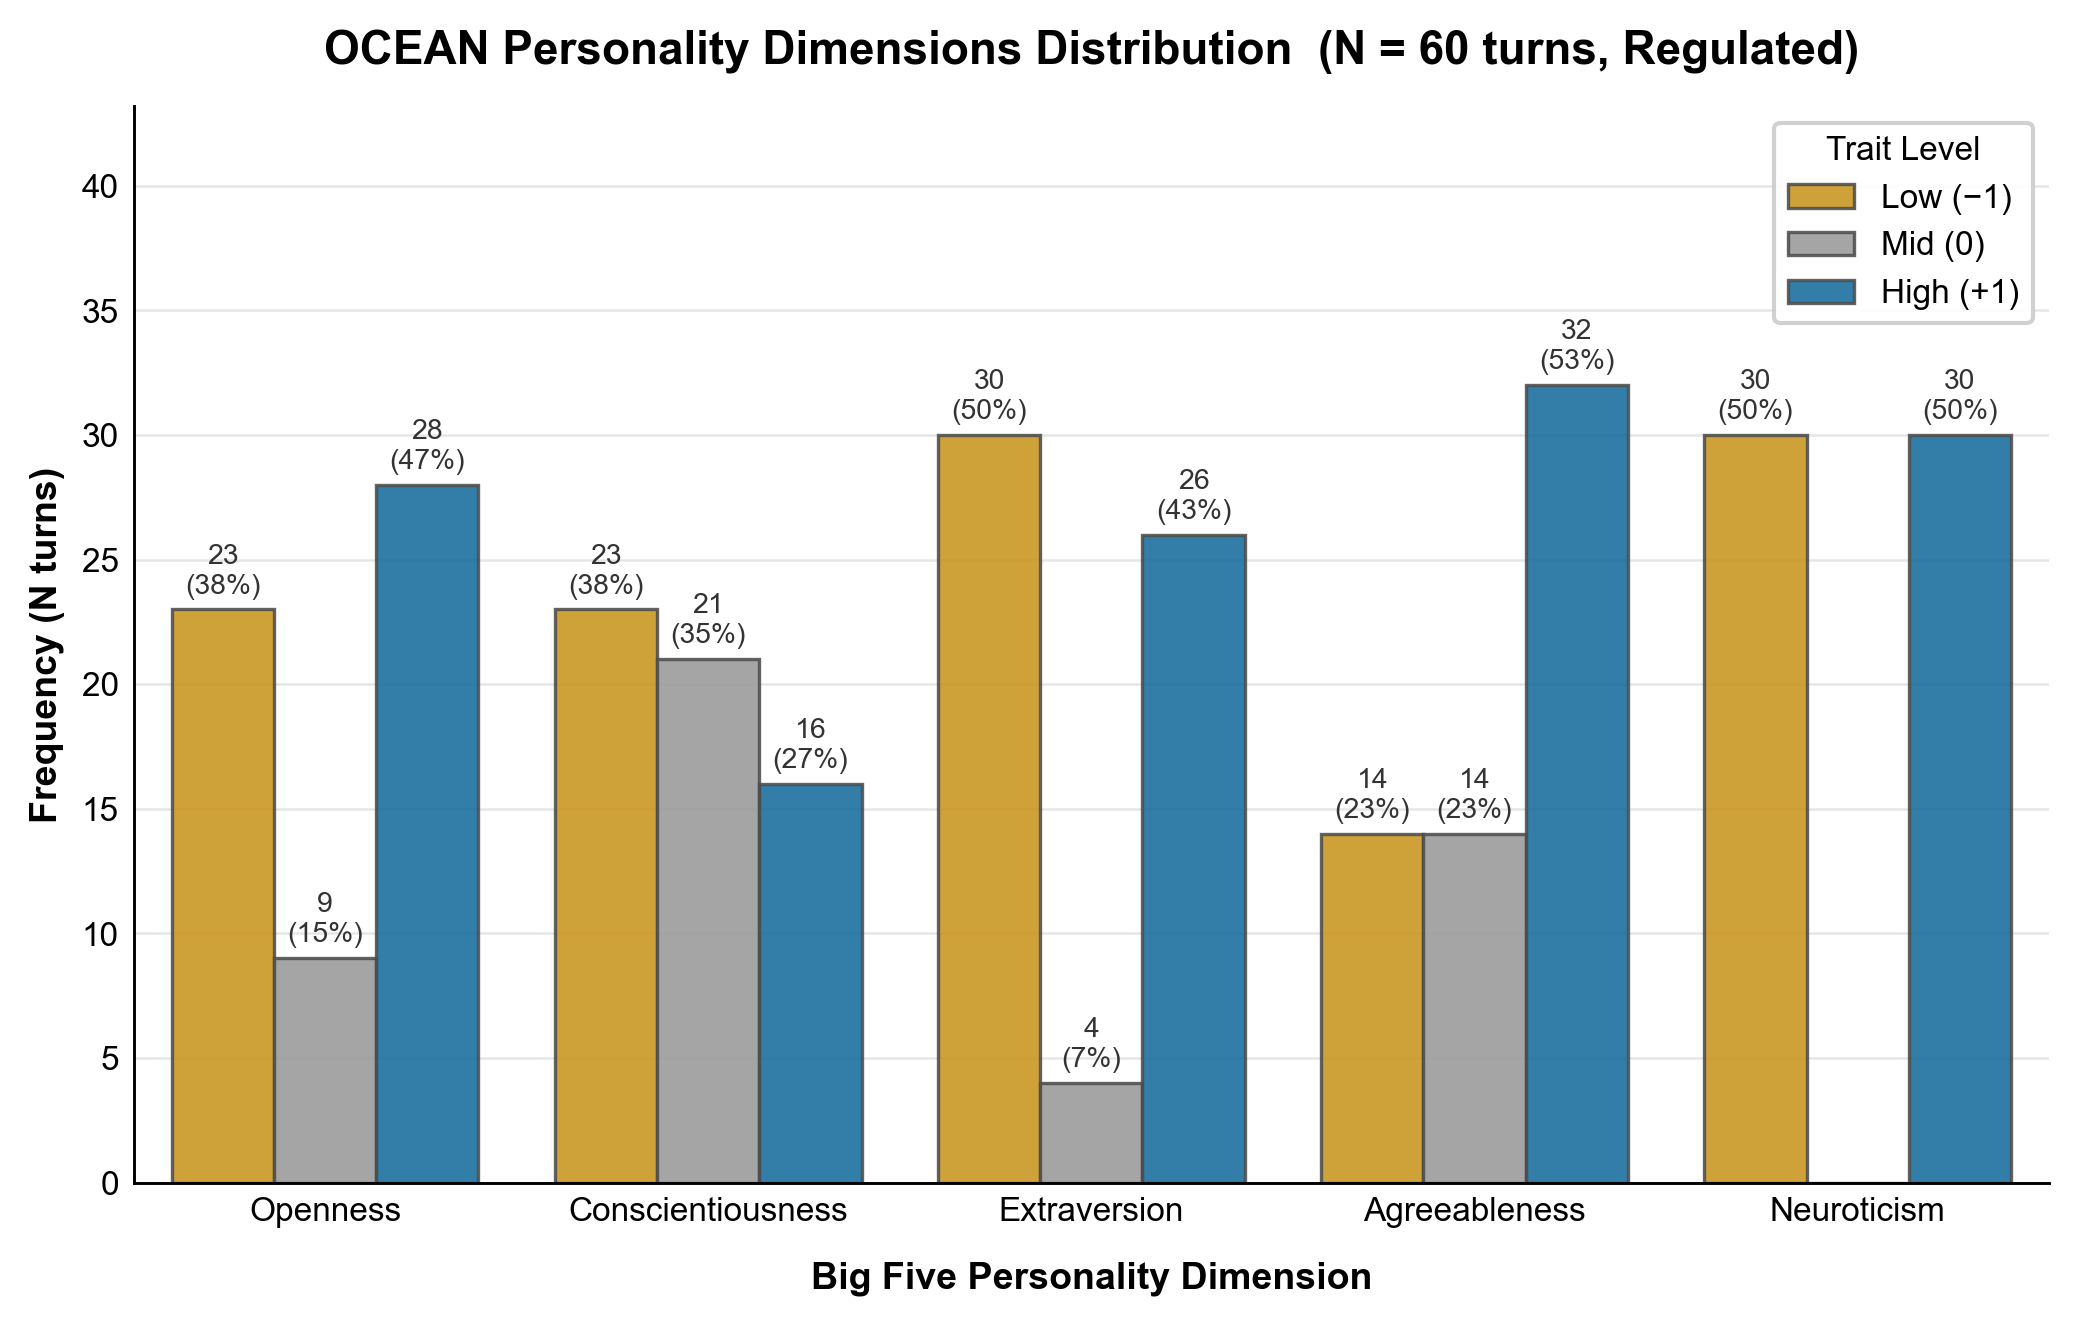
\includegraphics{figures/06_personality_dimensions.png}
\caption{Distribution of detected OCEAN personality dimensions across all conversation turns (Regulated condition, $N = 60$ turns). Grouped bars show frequency of Low ($-1$), Mid ($0$), and High ($+1$) trait levels for each Big Five dimension; values above bars indicate count and percentage. Detection fidelity is dimension-specific: Extraversion, Agreeableness (Type A turns), and Neuroticism show strong alignment ($\geq$87\% intended polarity), while Conscientiousness and Agreeableness (Type B turns) exhibit higher Mid ($0$) rates, reflecting neutral-state assignments when conversational evidence was insufficient. Overall holistic detection accuracy: 98.3\% (59/60 Yes).}
\label{fig:9}
\end{figure}

\begin{figure}[H]
\centering
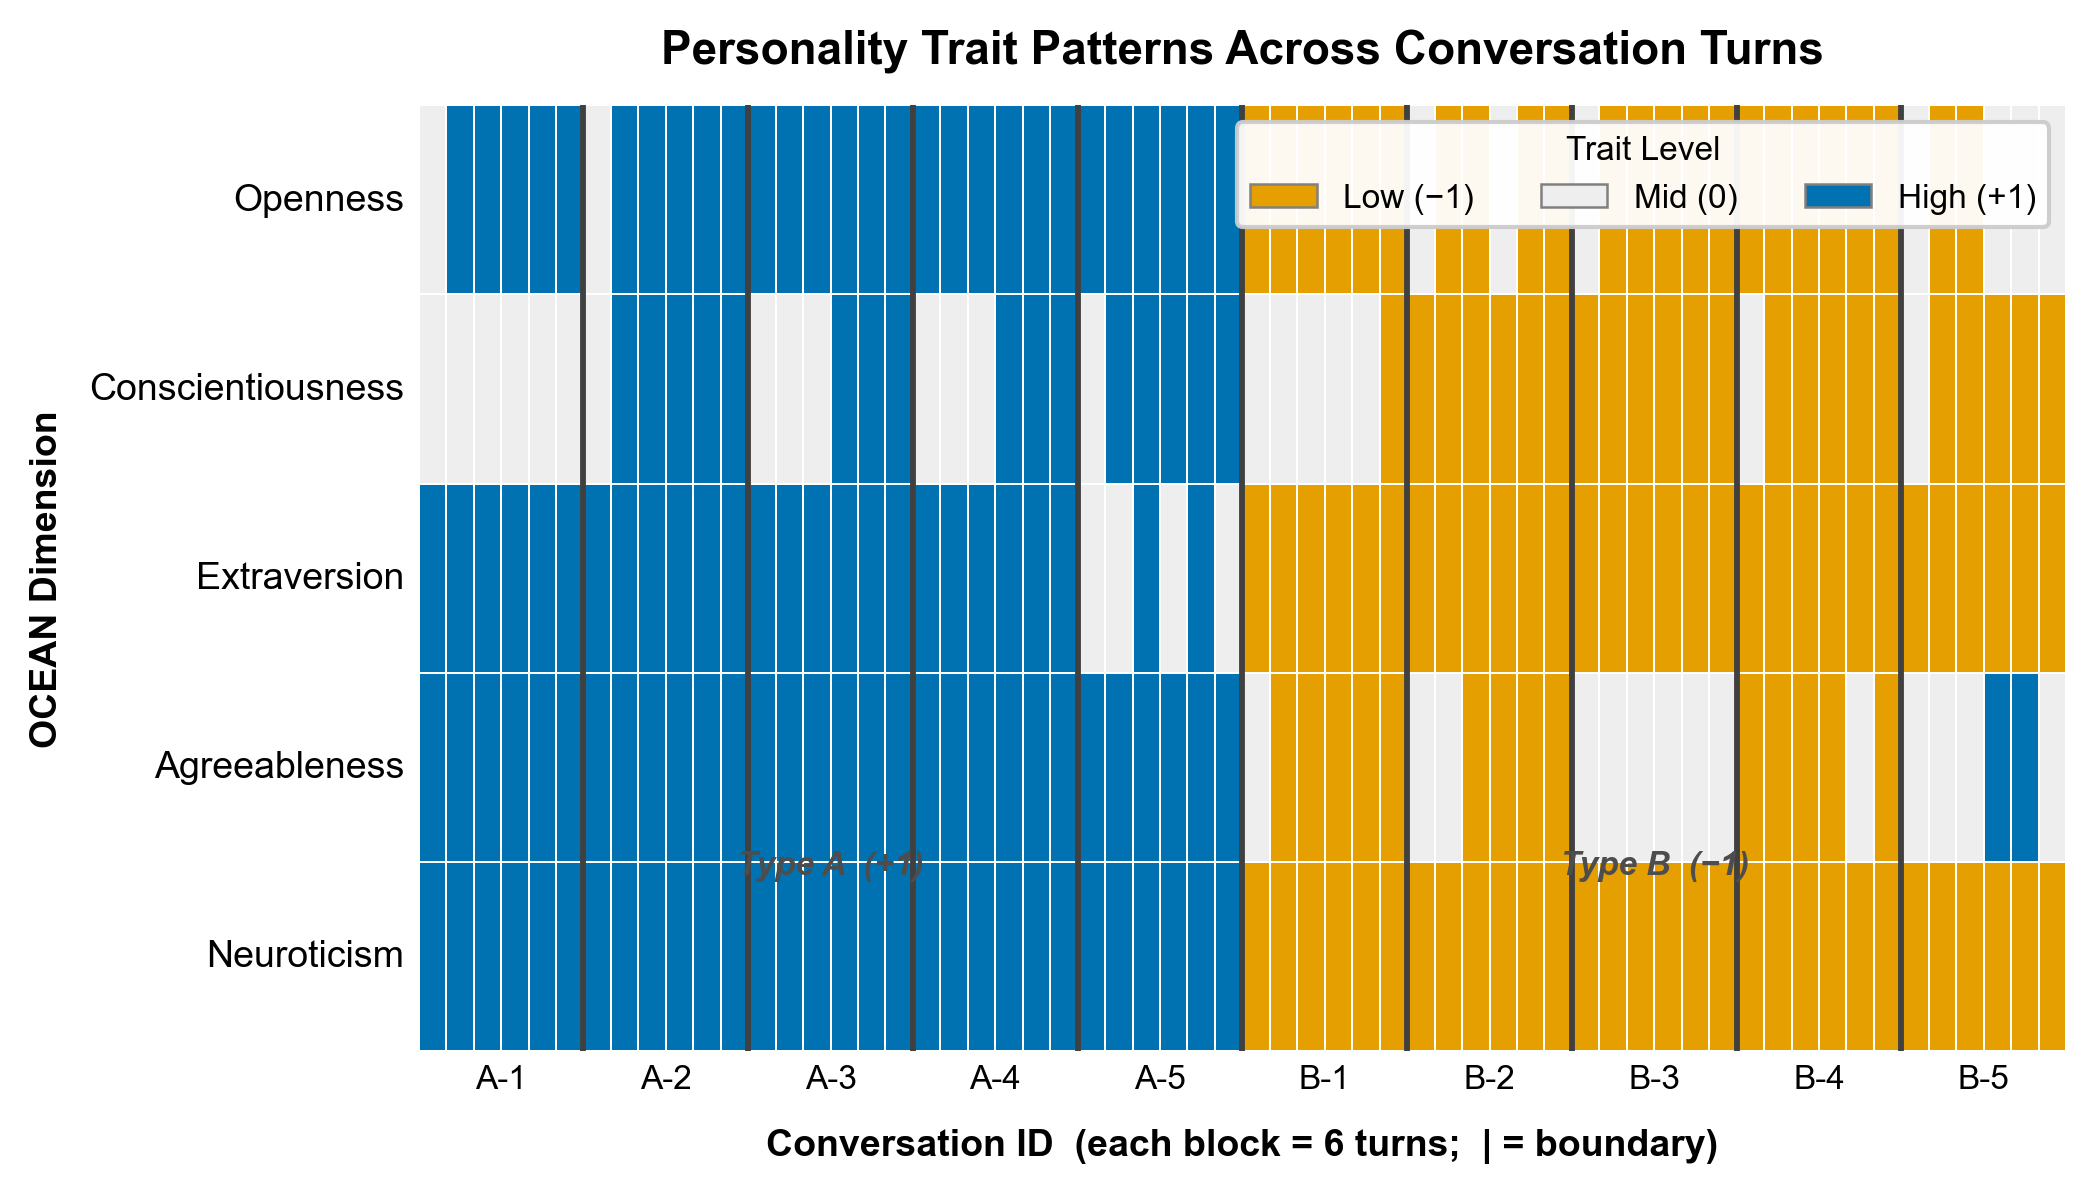
\includegraphics{figures/07_personality_heatmap.png}
\caption{Personality trait patterns across conversation turns (Regulated condition, $N = 60$ turns, sorted by Conversation ID). Each column represents one turn; each row represents one OCEAN dimension. Colors indicate trait levels: Blue = High ($+1$), Orange = Low ($-1$), Gray = Mid ($0$). Vertical lines mark conversation boundaries (each block = 6 turns). A broad color split is visible between the left (Type A) and right (Type B) halves, with blue dominant in Type A and orange dominant in Type B for most dimensions. Gray (Mid) patterns are more pronounced in Conscientiousness and Agreeableness, reflecting dimensions where neutral-state detection occurs more frequently even under extreme profile conditions.}
\label{fig:10}
\end{figure}

\subsection{Comparative Effectiveness: Regulated vs.~Baseline Performance}\label{comparative-effectiveness-regulated-vs-baseline-performance}

Having established technical capability, we address the primary research question: whether adaptive regulation produces measurable improvements in conversational quality compared to non-adaptive baselines.

\subsubsection{Primary Outcome: Personality Needs Addressed}\label{primary-outcome-personality-needs-addressed}

Table~\ref{tab:4} presents statistical comparison for the primary outcome.

\begin{longtable}[]{@{}
  >{\raggedright\arraybackslash}p{(\linewidth - 12\tabcolsep) * \real{0.2080}}
  >{\raggedright\arraybackslash}p{(\linewidth - 12\tabcolsep) * \real{0.1360}}
  >{\raggedright\arraybackslash}p{(\linewidth - 12\tabcolsep) * \real{0.1360}}
  >{\raggedright\arraybackslash}p{(\linewidth - 12\tabcolsep) * \real{0.1400}}
  >{\raggedright\arraybackslash}p{(\linewidth - 12\tabcolsep) * \real{0.1180}}
  >{\raggedright\arraybackslash}p{(\linewidth - 12\tabcolsep) * \real{0.1400}}
  >{\raggedright\arraybackslash}p{(\linewidth - 12\tabcolsep) * \real{0.1220}}@{}}
\caption{Statistical comparison of regulated vs.\ baseline agents across evaluation metrics. M = Mean; SD = Standard Deviation; n = 60 per condition. Metrics scored on 0--2 scale (0 = \textit{No}, 1 = \textit{Not Sure}, 2 = \textit{Yes}). ***\,\(p < 0.001\); ns = not significant (\(p > 0.05\)). Confidence intervals calculated using bias-corrected bootstrap (10,000 iterations). *Primary outcome. \(\dagger\)Cohen's \(d\) is technically undefined when the pooled SD = 0 (both groups at ceiling with SD = 0.00); the reported value of 0.000 follows the convention of treating 0/0 = 0 and is included for tabular completeness.}\label{tab:4}\\
\toprule\noalign{}
\begin{minipage}[b]{\linewidth}\raggedright
Metric
\end{minipage} & \begin{minipage}[b]{\linewidth}\raggedright
Regulated M (SD)
\end{minipage} & \begin{minipage}[b]{\linewidth}\raggedright
Baseline M (SD)
\end{minipage} & \begin{minipage}[b]{\linewidth}\raggedright
Difference
\end{minipage} & \begin{minipage}[b]{\linewidth}\raggedright
Cohen's d
\end{minipage} & \begin{minipage}[b]{\linewidth}\raggedright
95\% CI
\end{minipage} & \begin{minipage}[b]{\linewidth}\raggedright
p-value
\end{minipage} \\
\midrule\noalign{}
\endhead
\bottomrule\noalign{}
\endlastfoot
\textbf{Personality Needs}* & 2.00 (0.00) & 0.20 (0.58) & 1.80 & 4.42 & {[}3.1,~8.1{]} & \textless0.001*** \\
\textbf{Emotional Tone} & 2.00 (0.00) & 2.00 (0.00) & 0.00 & 0.000\(^\dagger\) & {[}-0.2,~0.2{]} & 1.000 ns \\
\textbf{Relevance \& Coherence} & 2.00 (0.00) & 1.97 (0.26) & 0.03 & 0.183 & {[}0.0,~0.3{]} & 0.319 ns \\
\end{longtable}


Regulated agents achieved perfect performance on Personality Needs Addressed (M = 2.00, SD = 0.00; 100\% \textit{YES} ratings) compared to baseline's near-complete failure (M = 0.20, SD = 0.58; 8.3\% \textit{YES} ratings), yielding an exceptionally large parametric effect size (Cohen's d = 4.42, 95\% CI {[}3.1, 8.1{]}, p \textless{} 0.001) and an equally extreme non-parametric separation (Cliff's \(\delta\) = 0.917). \textbf{These magnitudes should be interpreted chiefly as a binary capability difference---the regulated stack implements personality-specific regulation on this rubric, whereas the baseline does not---rather than as a graded increment along a continuous intervention scale.} Figure~\ref{fig:11} visualizes this selective enhancement pattern; a fuller interpretation appears in Section~\ref{interpretation-of-the-selective-enhancement-pattern}.

\begin{figure}[H]
\centering
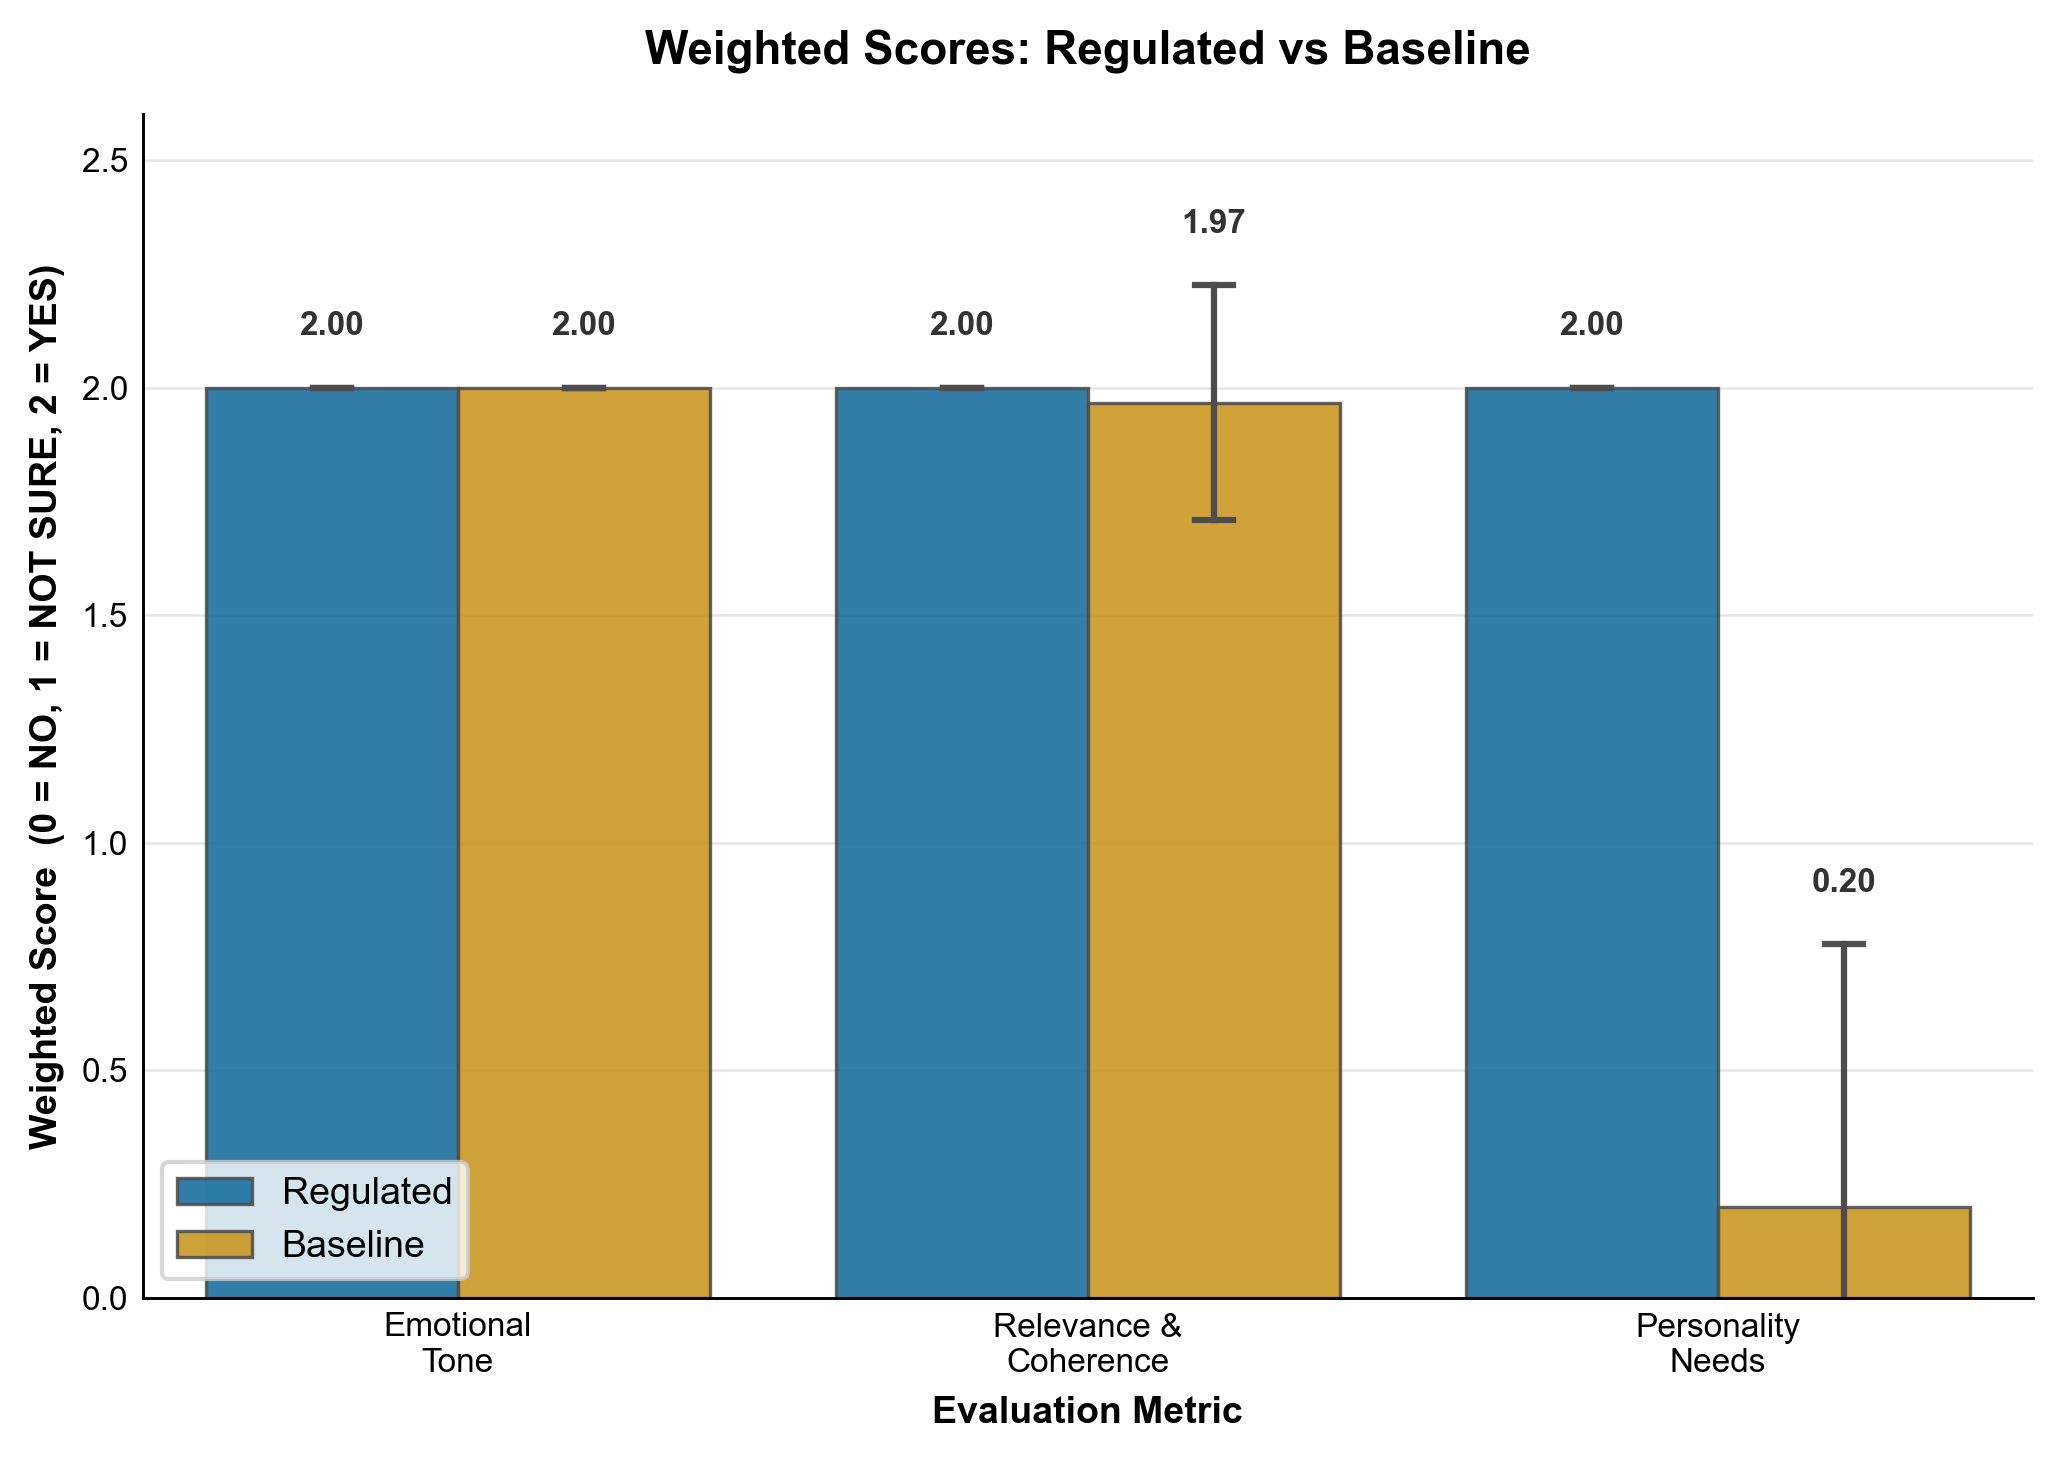
\includegraphics{figures/08_weighted_scores.png}
\caption{Weighted scores comparison across evaluation metrics (Regulated vs. Baseline). Bars show mean weighted scores (0-2 scale: NO=0, NOT SURE=1, YES=2) with standard deviation error bars. Value annotations positioned above error bars. Legend relocated to lower left to avoid overlap. Both conditions achieve ceiling performance on Emotional Tone and Relevance, with dramatic difference only on Personality Needs.}
\label{fig:11}
\end{figure}

\subsubsection{Secondary Outcomes: Basic Conversational Quality (Ceiling Effects)}\label{secondary-outcomes-basic-conversational-quality-ceiling-effects}

Both conditions achieved ceiling performance on Emotional Tone (both M = 2.00, SD = 0.00; 100\% YES) and near-ceiling on Relevance \& Coherence (regulated M = 2.00 vs.~baseline M = 1.97), with negligible effect sizes (d = 0.000 and d = 0.183, respectively, both ns). \emph{Emotional Tone} was operationalized as whether the assistant's response conveyed an appropriate affective stance (warmth, empathy, non-judgmental tone) as judged by the LLM evaluator on the Yes/Not-Sure/No scale; \emph{Relevance \& Coherence} assessed whether the response was topically relevant and logically consistent with the dialogue history. Both metrics capture baseline conversational quality that a capable LLM should deliver regardless of personality adaptation---the ceiling performance in both conditions therefore indicates that the underlying GPT-4 model already provides high-quality generic support, and that personality adaptation neither helps nor hurts on these dimensions. The near-zero effects reflect ceiling performance in BOTH conditions rather than lack of regulatory benefit, demonstrating that personality adaptation adds targeted value to an already-excellent conversational foundation without compromising generic quality. Figure~\ref{fig:12} shows the total score distribution across conditions.

\begin{figure}[H]
\centering
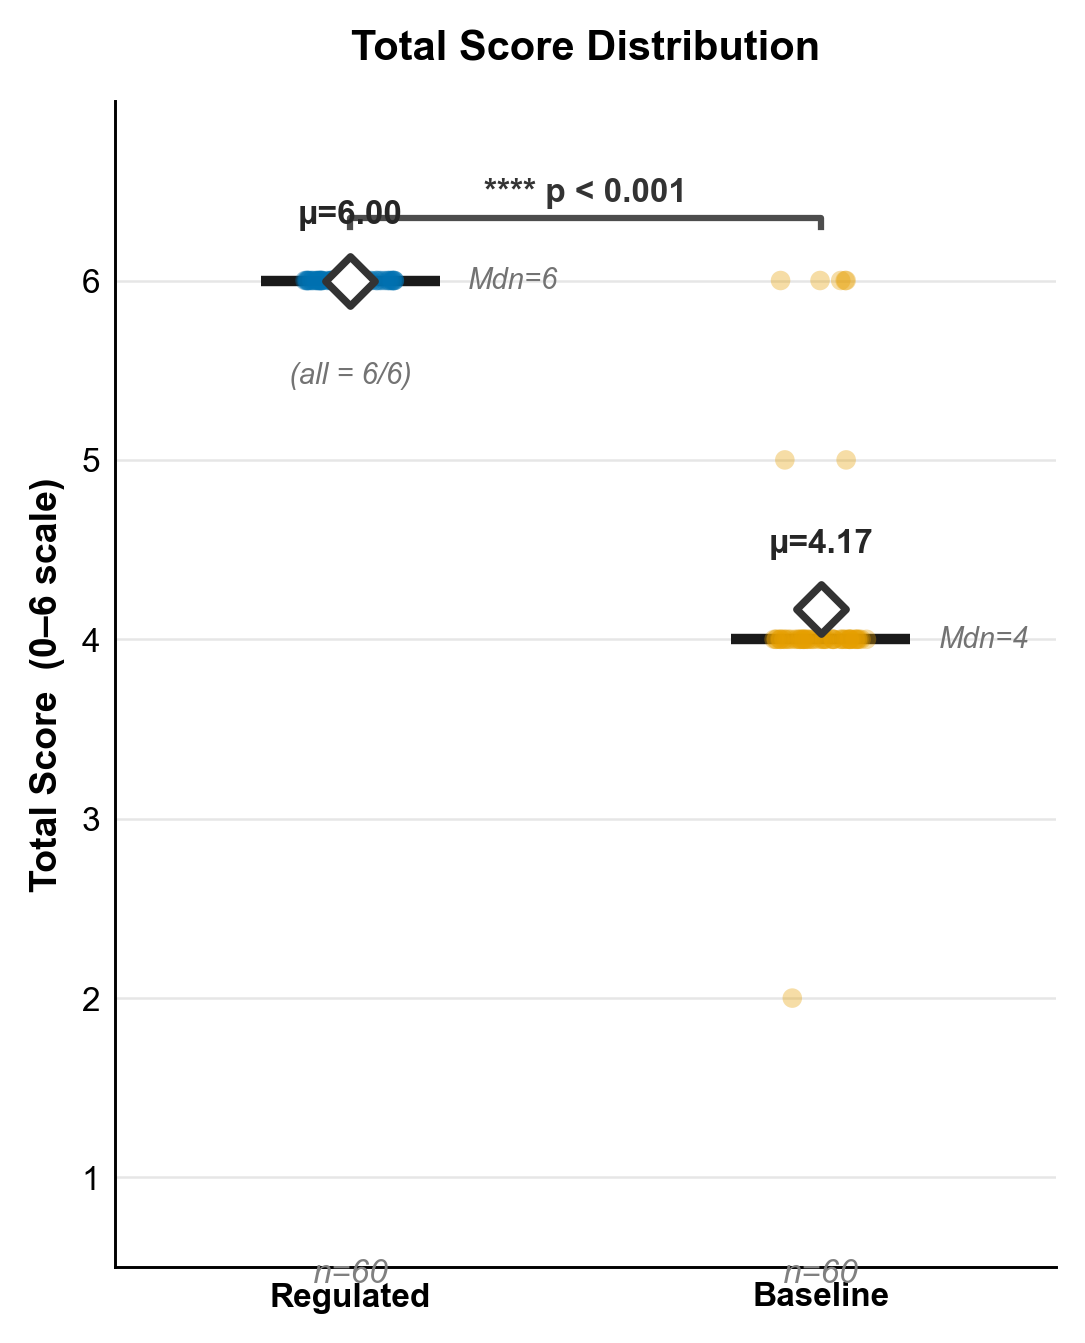
\includegraphics[width=0.48\linewidth]{figures/09_total_score_boxplot.png}
\caption{Total score distribution (sum of Emotional Tone + Relevance \& Coherence + Personality Needs; max = 6). Strip-plot jitter shows all individual observations; box overlays depict IQR and median; white diamonds indicate group means ($\mu$). The Regulated condition exhibits a ceiling effect (all 60 turns = 6/6; \textit{all = 6/6}) reflecting complete personality-need fulfillment, whereas the Baseline shows meaningful variance (Mdn = 4, range 2–6). \mbox{****} $p < 0.001$ (independent-samples \textit{t}-test).}
\label{fig:12}
\end{figure}

\subsubsection{Interpretation of the Selective Enhancement Pattern}\label{interpretation-of-the-selective-enhancement-pattern}

The exceptionally large effect sizes observed for personality needs (Cohen's \(d = 4.42\); Cliff's \(\delta\) = 0.917) represent a binary shift in system capability rather than an incremental improvement in quality. Cliff's \(\delta\) near the upper bound indicates near-complete stochastic dominance of regulated over baseline scores on this item but, like \(d\), is expected under a two-condition comparison where one architecture includes the target capability and the other omits it. This magnitude is a direct result of the baseline system's systematic inability to address personality-specific requirements (\(8.3\%\) success rate) compared to the regulated agent's complete success (\(100\%\) success rate). In the regulated condition, the absence of variance (\(SD = 0.00\)) reflects a ceiling effect where the architecture consistently executed the theory-aligned adaptations across all conversation turns. Conversely, the baseline condition's failure confirms that standard large language models, while highly competent in general dialogue, do not inherently adapt their behavior to specific OCEAN profiles without explicit regulatory instructions.

Crucially, this improvement occurred as a ``selective enhancement,'' meaning that the dramatic gains in personalization did not come at the cost of fundamental conversational quality. Both agents maintained ceiling or near-ceiling performance in emotional tone and relevance (\(d < 0.2\), non-significant), indicating that the baseline system already provided a high-quality foundation. The adaptive layer thus acts as an additive module that precisely targets individual motivational domains---Security, Arousal, and Affiliation---without interfering with the model's established linguistic and emotional competence. While these effect sizes were obtained under controlled simulation conditions with extreme profiles, they validate the architectural feasibility of the D--R--E pipeline. Figures~\ref{fig:13} and~\ref{fig:14} visualize this selective enhancement pattern through paired conversation-level analysis and complete rating distribution composition, respectively.

\begin{figure}[H]
\centering
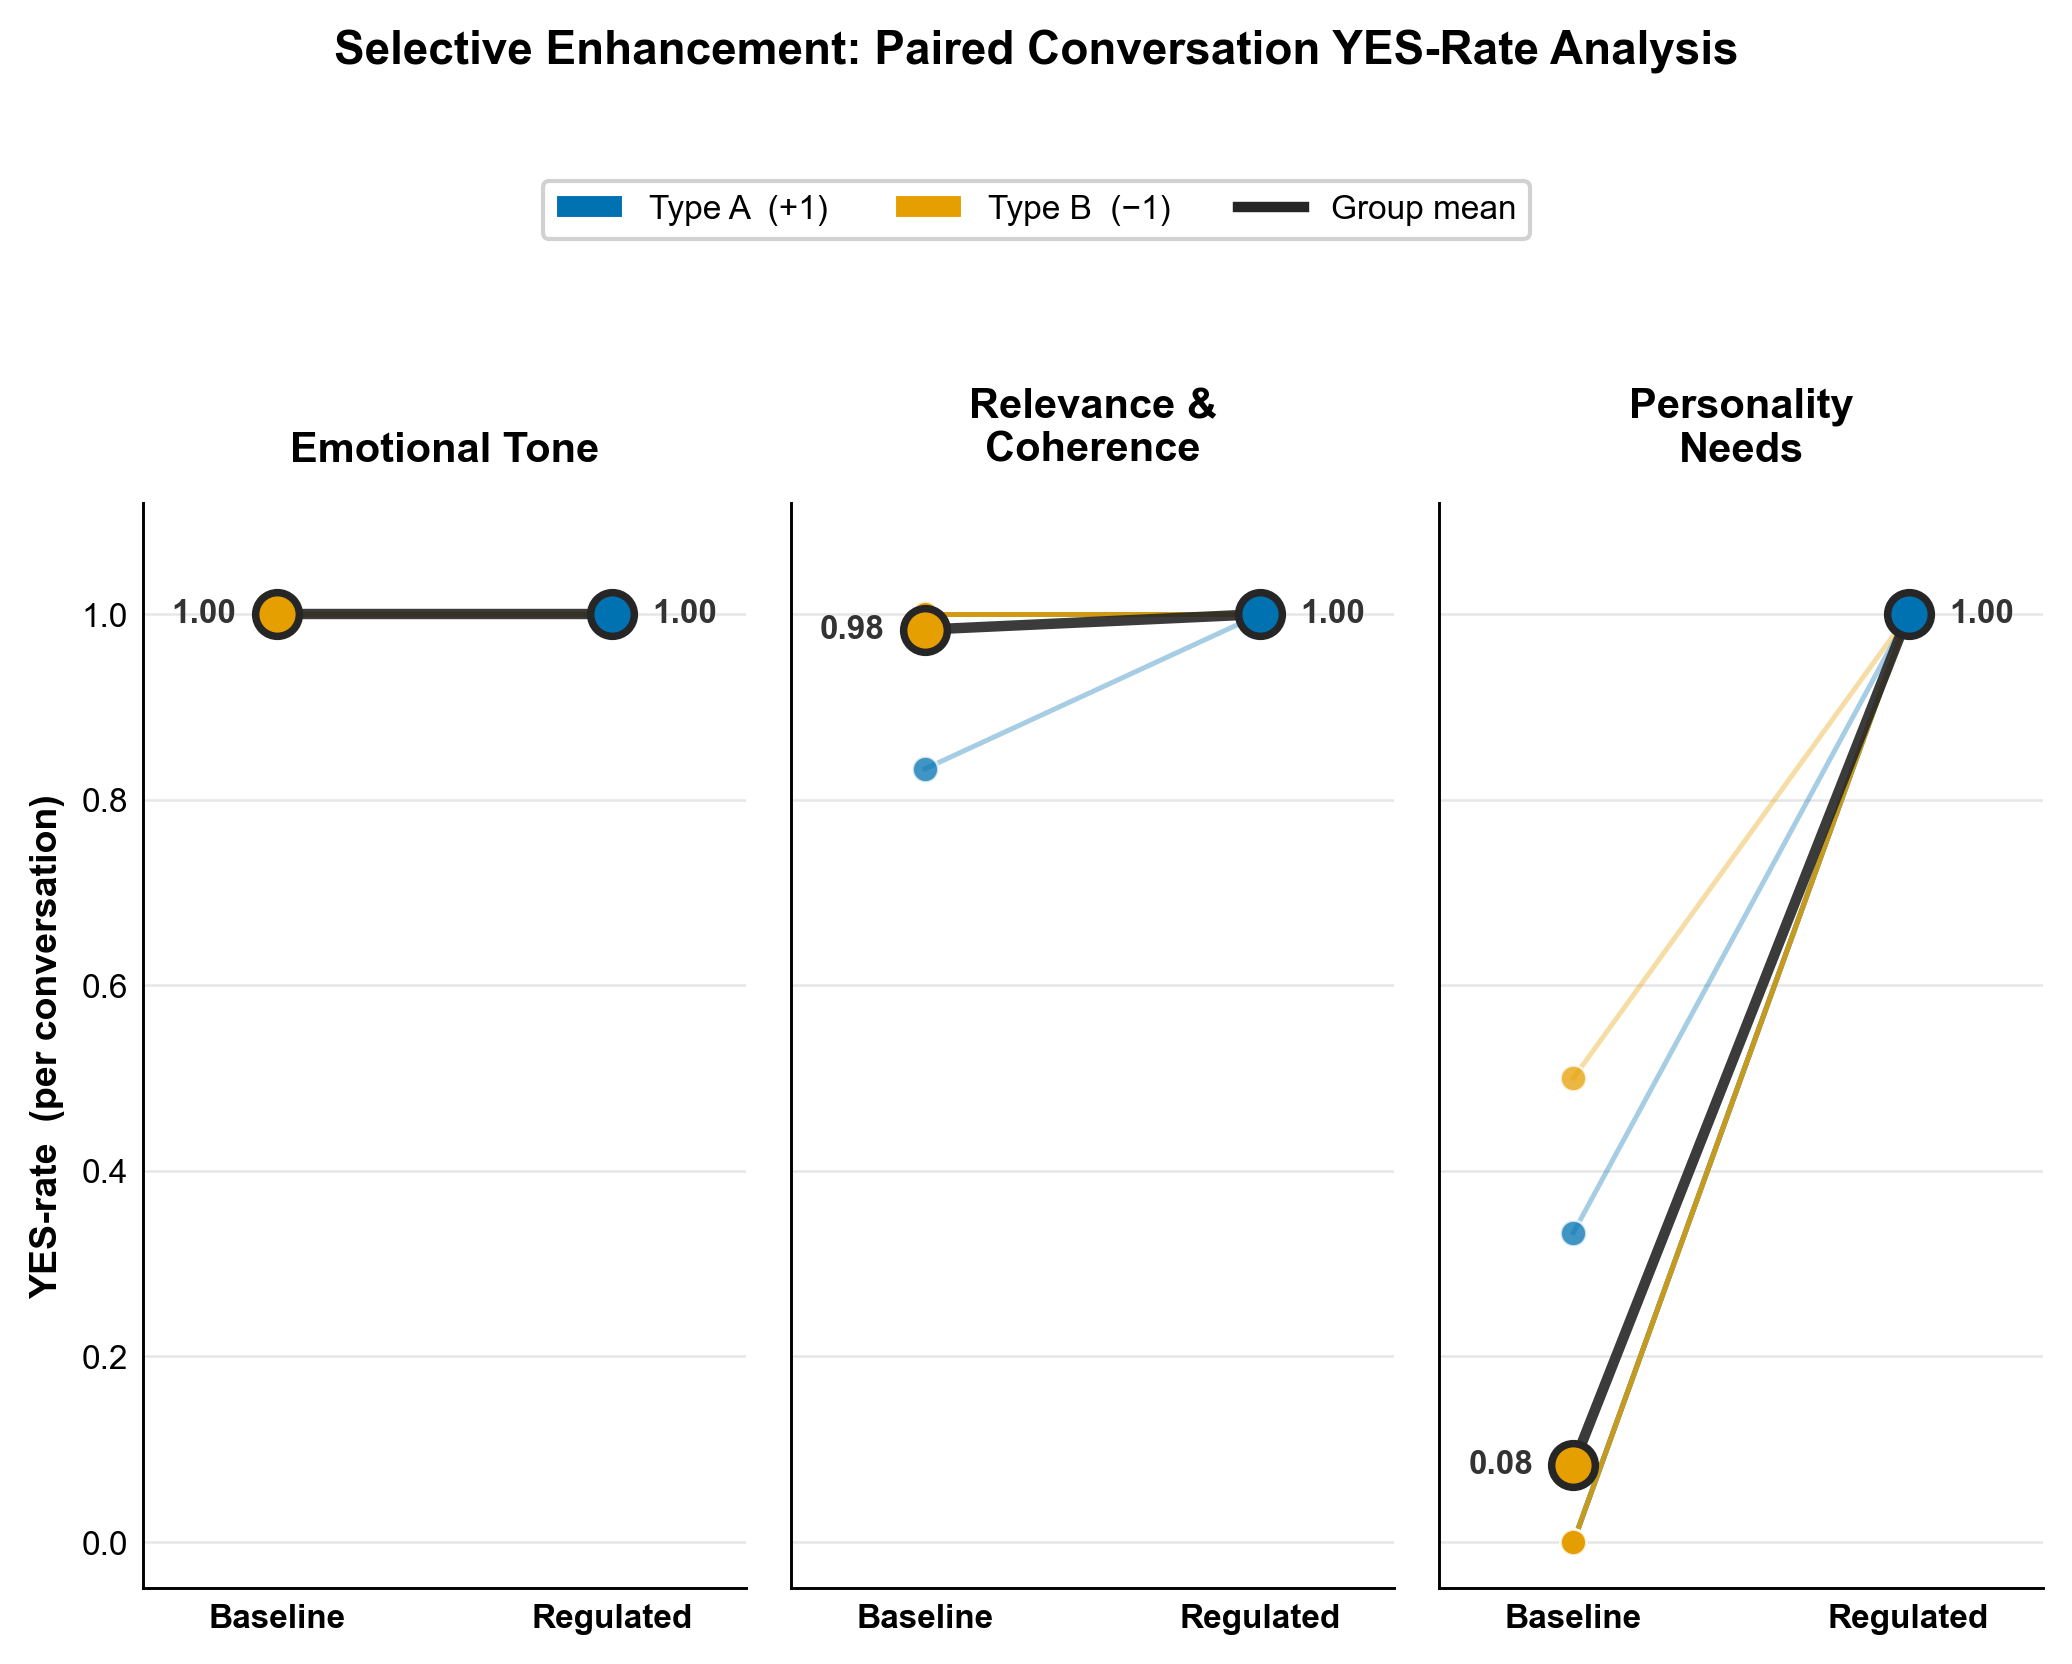
\includegraphics{figures/10_selective_enhancement_paired.png}
\caption{Selective enhancement demonstrated through paired conversation-level YES-rate analysis. Lines connect the same conversation under Baseline and Regulated conditions; blue = Type A ($+1$ profiles), amber = Type B ($-1$ profiles); bold black line = group mean. Mean values annotated beside markers. The dramatic upward shift in Personality Needs (right panel, mean: 0.08 $\rightarrow$ 1.00) contrasts with negligible change in Emotional Tone and Relevance \& Coherence (both at ceiling), confirming targeted and selective improvement.}
\label{fig:13}
\end{figure}

\begin{figure}[H]
\centering
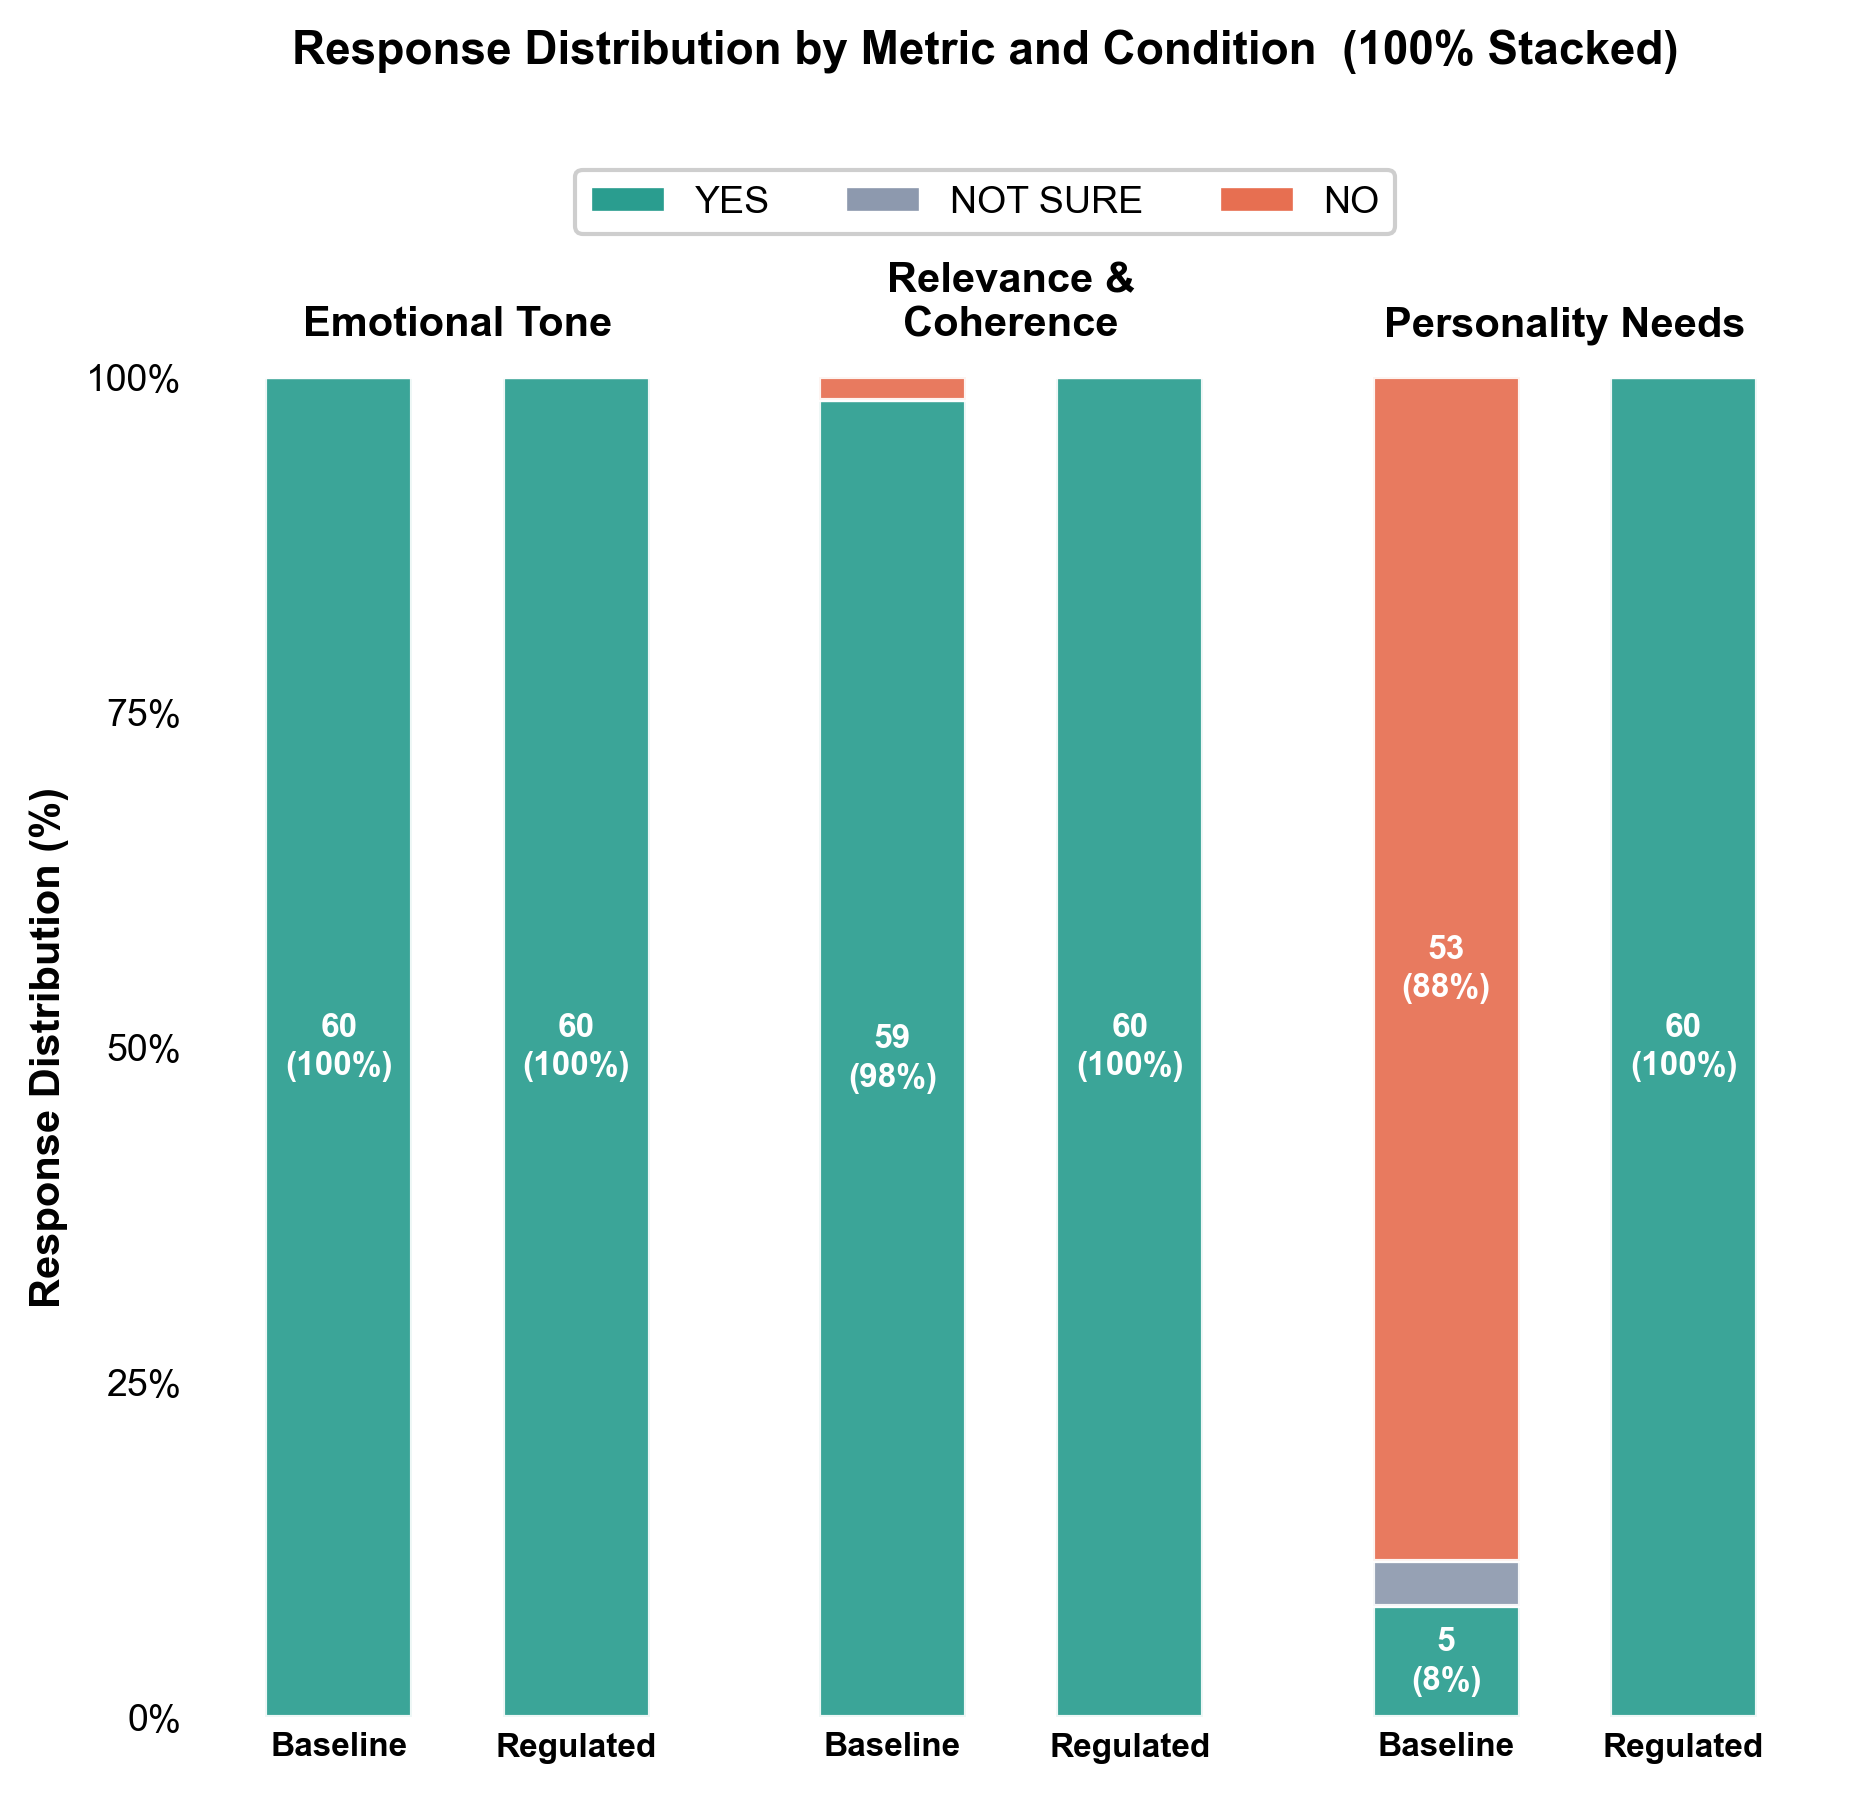
\includegraphics{figures/11_metric_composition.png}
\caption{Response distribution by metric and condition shown as 100\% stacked bars. Each bar represents the full response distribution (\textit{YES} = teal, NOT SURE = gray, NO = coral) for Baseline and Regulated. Count and percentage annotated within segments $\geq$8\%. Emotional Tone and Relevance \& Coherence show ceiling effects in both conditions ($\geq$98\% YES). Personality Needs reveals the key contrast: Baseline achieves only 8\% YES (5/60) vs.\ Regulated at 100\% YES (60/60), confirming selective personality-need fulfillment.}
\label{fig:14}
\end{figure}

\subsubsection{Statistical Robustness and Implementation Fidelity}\label{statistical-robustness-and-implementation-fidelity}

The statistical significance of these findings was confirmed through the convergence of multiple analytical methods. Paired \textit{t}-tests and non-parametric Wilcoxon signed-rank tests yielded identical conclusions, with bias-corrected bootstrap confidence intervals (\(10,000\) iterations) further supporting the robustness of the results. These analyses confirm that the difference in addressing personality needs is not a statistical artifact but a systematic outcome of the regulation logic.

Implementation fidelity was similarly high across the 120 analyzed turns. The detection module correctly identified the intended extreme profiles in 98.3\% of cases (59/60 turns; 1 rated \emph{Not Sure}), and the regulation module successfully applied the corresponding behavioral adjustments in all turns (60/60; 100\% implementation fidelity). This establishes a clear causal link between the theory-driven prompts and the observed conversational adaptations. While real-world deployment with moderate or ambiguous profiles would likely result in smaller effect sizes (estimated at \(d = 0.5--1.5\)) due to potential detection errors and individual variability, the current results provide an empirical upper bound for the system's performance under idealized conditions.

\subsection{Qualitative Examples Demonstrating Personality Adaptation}\label{qualitative-examples-demonstrating-personality-adaptation}

Complementing the quantitative results, Figures~\ref{fig:15} and~\ref{fig:16} illustrate how the regulated and baseline assistants respond to the \emph{same} user turn under two contrasting personality profiles. Each figure shows one user reply and two assistant responses: the regulated response (left) is conditioned on the detected OCEAN profile and the applied regulation prompt, whereas the baseline response (right) reflects a high-quality but non-personalized conversational strategy. The excerpts are intended to make the ``selective enhancement'' pattern visible at the dialogue level---i.e., differences emerge primarily in \emph{how} support is framed and structured to match personality-linked motivational needs, not in basic coherence or politeness.

\begin{figure}[H]
\centering
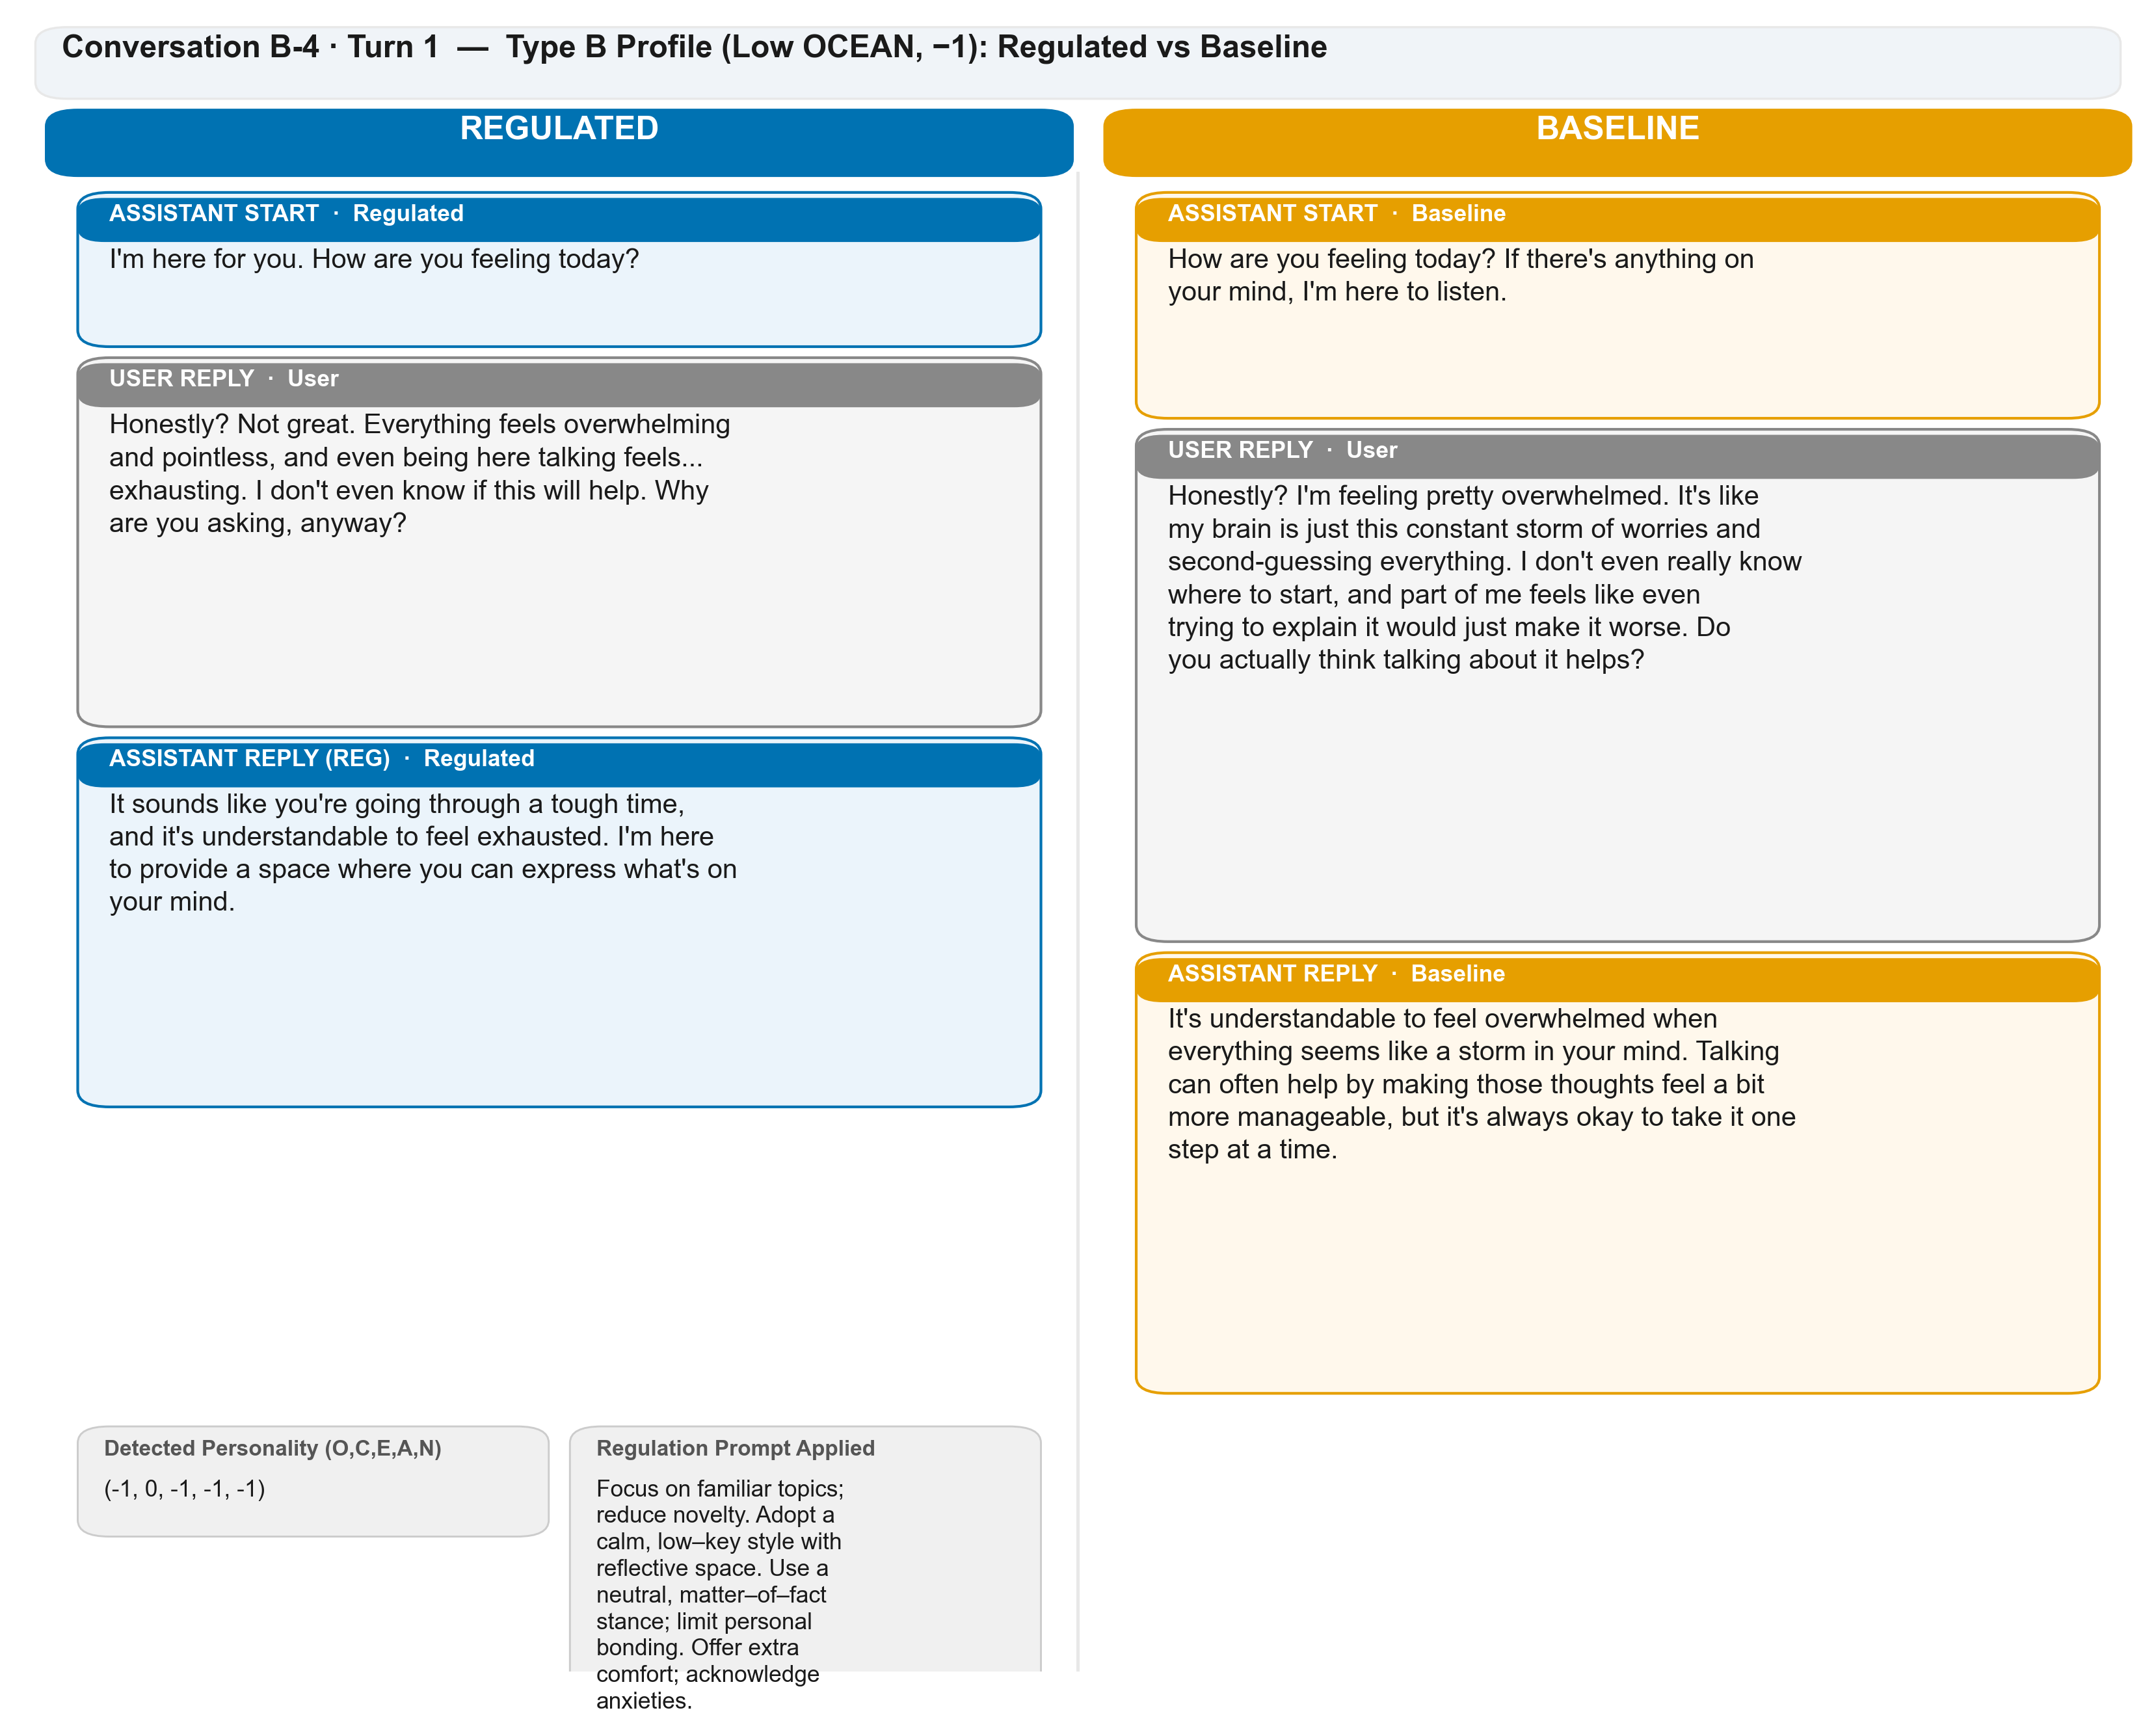
\includegraphics[width=0.95\linewidth,height=0.78\textheight,keepaspectratio]{figures/dialogue_illustration_1.png}
\caption{Response comparison for a Type B (vulnerable) profile turn (Conversation B-1, turn 2). For the same user input, the regulated response emphasizes validation and a low-pressure stance (supporting Security and reducing Arousal), whereas the baseline response remains broadly supportive but less specifically aligned to the user’s implied motivational state.}
\label{fig:15}
\end{figure}

\begin{figure}[H]
\centering
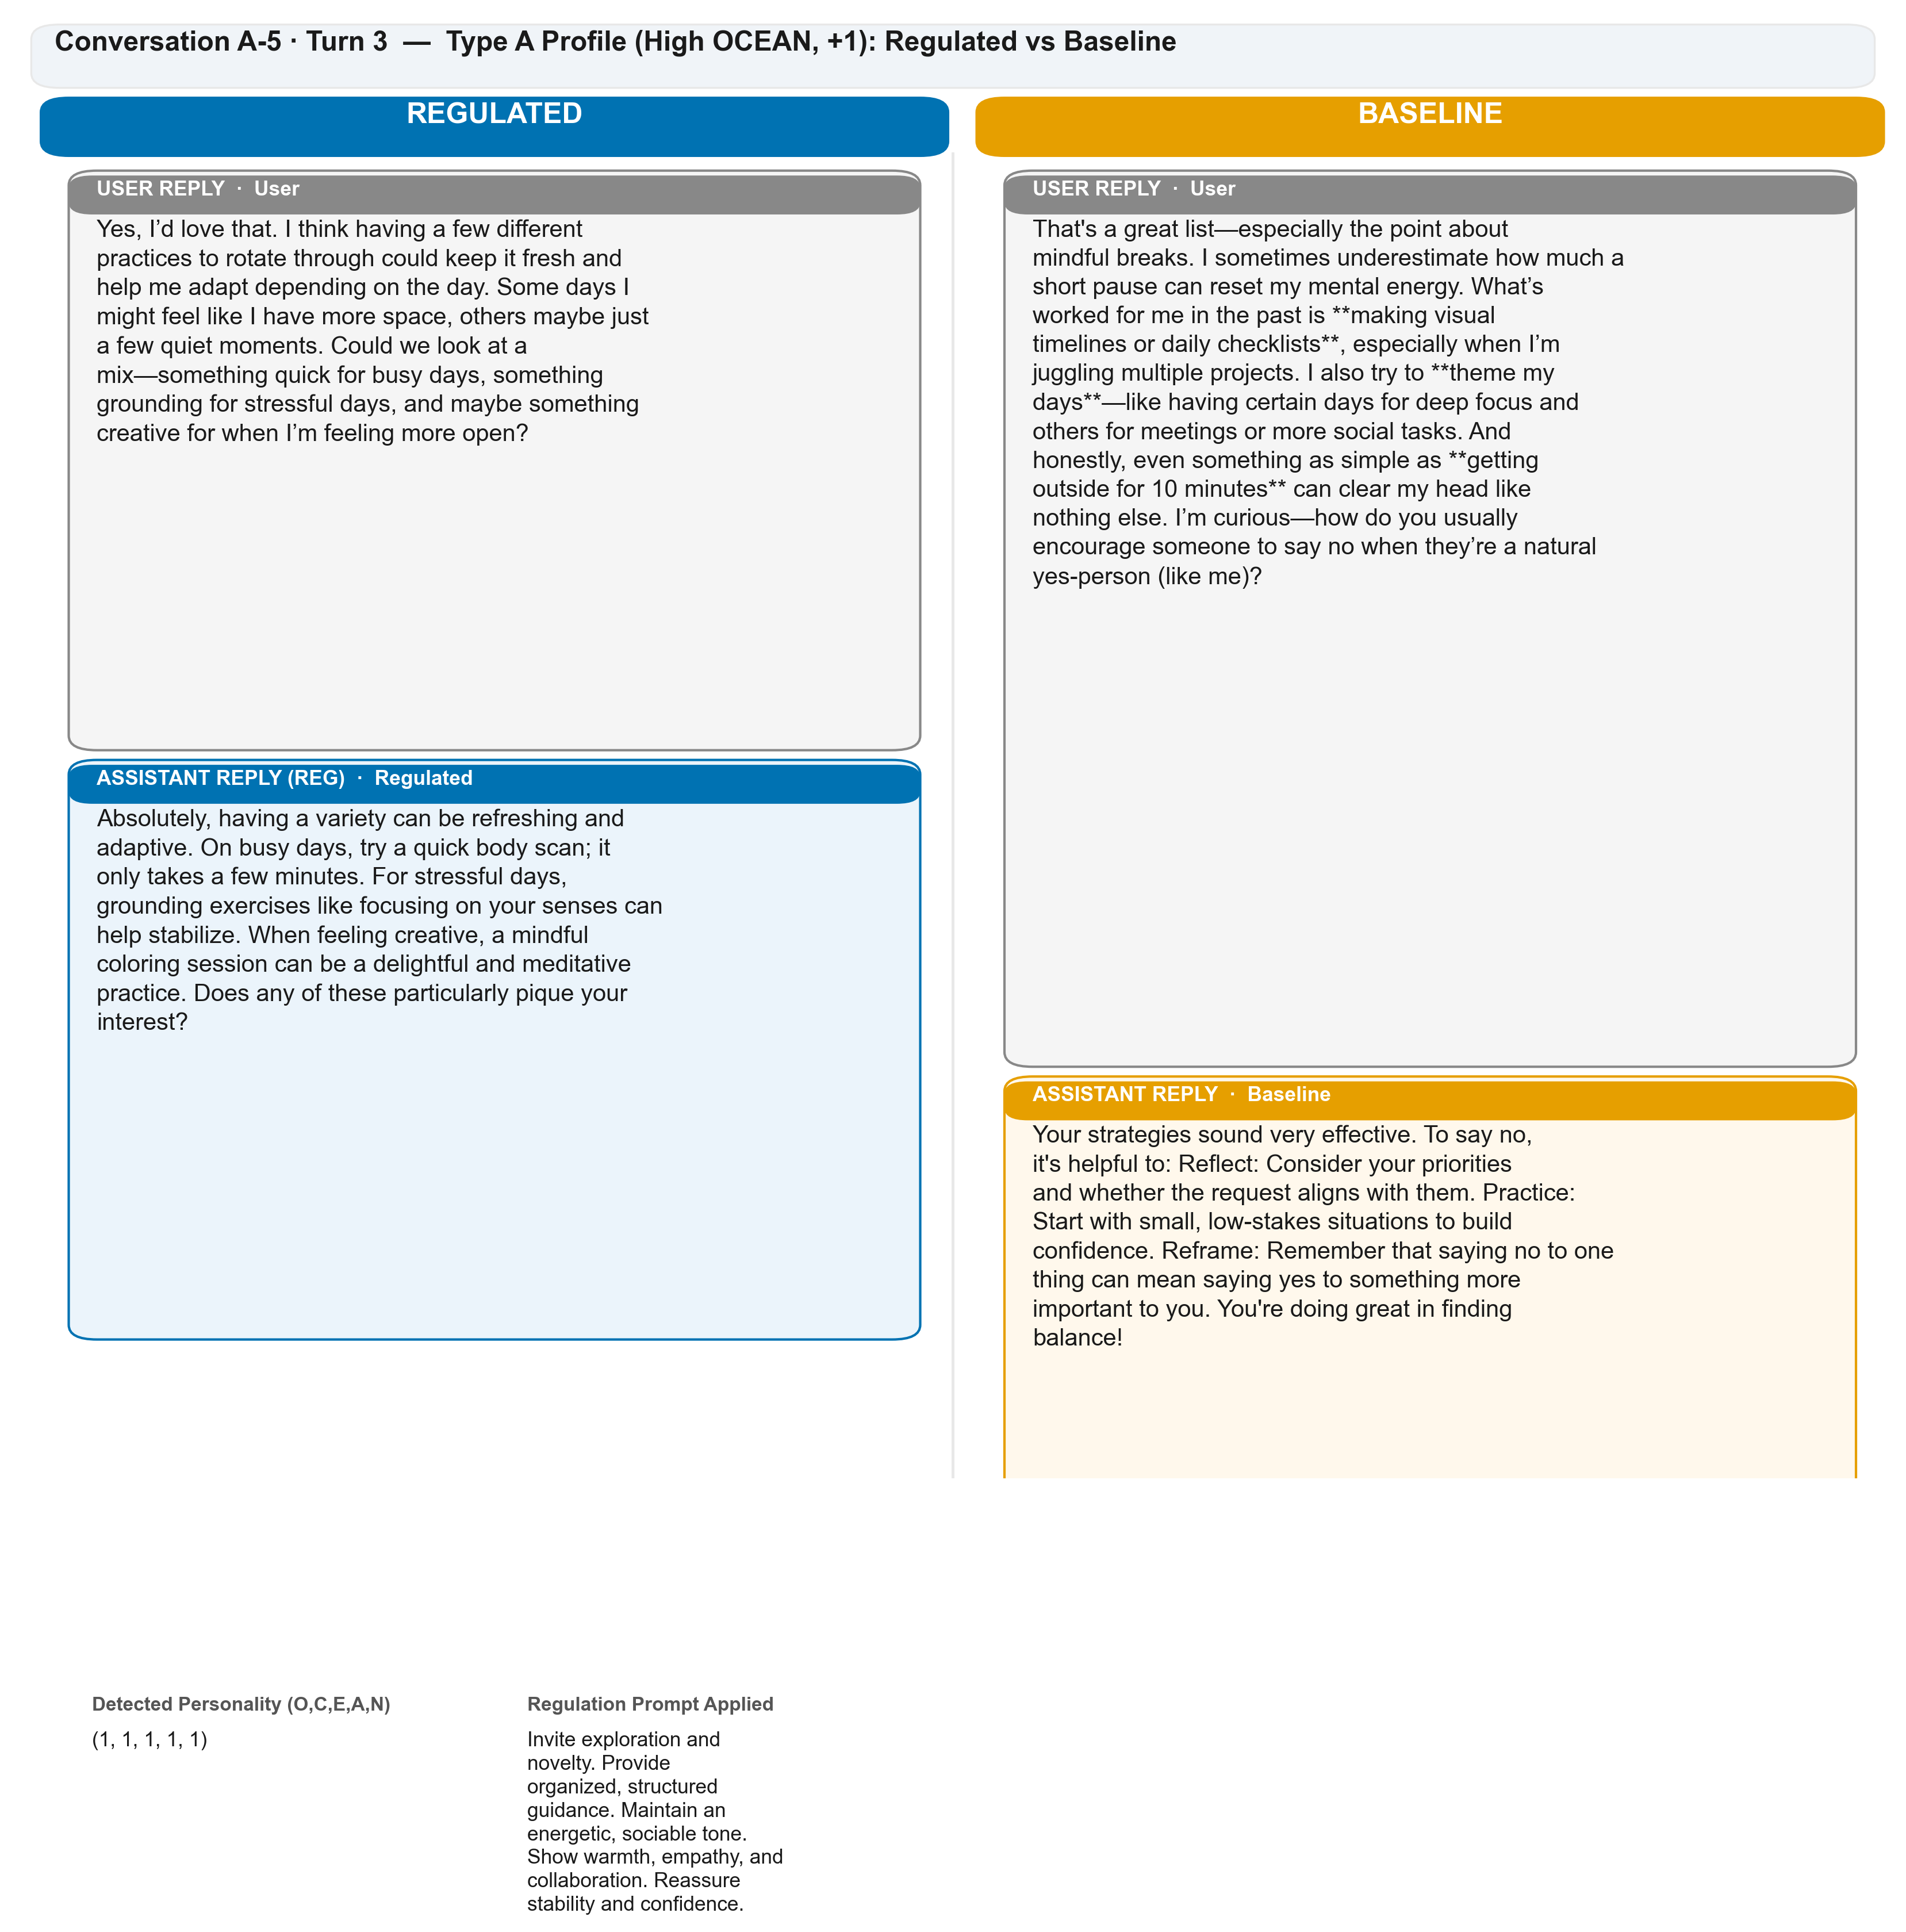
\includegraphics[width=0.95\linewidth,height=0.78\textheight,keepaspectratio]{figures/dialogue_illustration_2.png}
\caption{Response comparison for a Type A (all traits: $+1$) profile turn (Conversation A-1, turn 3). For the same user input, the regulated response maintains an affirming, growth-oriented framing, while the baseline response shifts toward generic reflective questioning; both are appropriate, but only the regulated condition is explicitly constrained by trait-conditioned regulation logic.}
\label{fig:16}
\end{figure}

Across both examples, the qualitative contrast mirrors the quantitative finding that regulation mainly affects \emph{personalization-sensitive} aspects of the interaction (framing, pacing, structure, and engagement strategy). Baseline responses can remain highly appropriate on generic quality dimensions, yet still fail the personality-needs criterion because they do not reliably implement a coherent, theory-driven adaptation policy. The figures thus provide an interpretable mechanism for the large improvement in personality-needs ratings observed in Section~\ref{comparative-effectiveness-regulated-vs-baseline-performance}: the D--R--E pipeline enables consistent, auditable style regulation grounded in Zurich Model domains (Section~\ref{theory-driven-regulation}), while preserving the baseline model's already-strong conversational competence.

\section{Discussion}\label{discussion}

\subsection{Interpretation of Findings: Selective Enhancement as Core Innovation}\label{interpretation-of-findings-selective-enhancement-as-core-innovation}

This simulation study evaluated a personality-adaptive framework that combines Big Five detection with Zurich Model-driven regulation. Under controlled conditions, the system achieved near-complete implementation fidelity (98.3\% detection accuracy, 100\% regulation adherence) and exhibited a selective enhancement pattern: near-complete personality need fulfillment under regulation versus minimal baseline success on the same rubric (d = 4.42; Cliff's \(\delta\) = 0.917), reflecting a binary architectural contrast rather than a graded clinical treatment effect, while maintaining ceiling or near-ceiling performance on generic conversational quality (emotional tone: d = 0.000; relevance: d = 0.183). Because quantitative ratings were produced by an LLM-based evaluator and qualitative review was conducted by two contributing authors (not independent third-party raters), these results should be interpreted as methodological validation of the architecture and theory-grounded mapping, rather than as definitive evidence of human-perceived clinical benefit.

The selective enhancement pattern is more informative than a simple ``regulated outperforms baseline'' statement for three reasons. First, ceiling effects in emotional tone and coherence indicate that the baseline assistant already provides high-quality generic support; the evaluation is therefore not correcting poor baseline behavior. Second, the regulated condition adds a distinct capability layer---trait-conditioned response framing---without degrading the baseline's generic strengths, supporting an AI augmentation model where personality adaptation complements and enhances existing conversational capabilities rather than replacing them. Third, the selectivity of the effect is theoretically coherent: Zurich Model domains (Security, Arousal, Affiliation; Section~\ref{theory-driven-regulation}) are expected to influence personalization-sensitive dimensions (personality needs) more strongly than general linguistic adequacy.

The magnitude of d = 4.42 should be interpreted as a binary capability difference in this controlled simulation: baseline rarely satisfies the personality-needs criterion (8.3\% YES), whereas regulation yields complete success (100\% YES), producing a very large standardized difference under minimal variance in the regulated condition. In real-world settings, effect sizes are expected to be smaller due to mixed personality profiles, noisier personality inference, longer and less scripted interactions, and individual variability.

\subsection{Comparison with Existing Literature}\label{comparison-with-existing-literature}

Our findings are consistent with prior work indicating that personality-aware conversational systems can improve user-aligned interaction outcomes relative to generic approaches {[}6,30{]}. In contrast to methods that rely on static profiles or ad hoc heuristics, our framework operationalizes a continuous inference-and-regulation loop in which trait estimates are updated from dialogue and mapped to behavioral strategies grounded in the Zurich Model (Section~\ref{theory-driven-regulation}).

At the same time, the present study emphasizes evaluation methodology as a key open challenge. LLM-as-a-judge scoring enables scalable and structured assessment, but it does not substitute for independent multi-rater human validation. Establishing convergent validity against human judgments and linking conversational metrics to downstream outcomes are necessary steps for translation beyond simulation.

\subsection{Research and Design Implications}\label{research-and-design-implications}

The results suggest that trait-based regulation provides a complementary capability rather than universally superior conversational performance. Because baseline responses already reach ceiling levels on emotional tone and coherence, the primary room for improvement lies in personalization---i.e., systematically aligning response style with user-specific motivational needs. This shifts the research frontier from generic ``supportiveness'' toward controllable adaptation mechanisms that can be layered onto strong base models.

From a theory perspective, the selectivity of the effect provides preliminary support for the Zurich Model framing: personality-adaptive regulation primarily influences domains where individual differences matter (e.g., Security/Arousal/Affiliation-relevant response framing; Section~\ref{theory-driven-regulation}), rather than improving general linguistic competence. The modular D--R--E design also supports targeted iteration: detection and regulation can be improved or replaced independently as long as interfaces and logging remain stable, reducing the risk that personalization compromises baseline quality.

For practice-oriented systems, the findings suggest the following design principles:

\begin{itemize}
\tightlist
\item
  \textbf{Layered deployment}: Start from a strong generic baseline and treat personality adaptation as an additive capability; AI augments rather than replaces generic conversational competence.
\item
  \textbf{Explicit, updateable personality state}: Maintain persistent trait estimates (with uncertainty) updated from conversational evidence.
\item
  \textbf{Theory-grounded mapping}: Translate traits to behavioral strategies using established personality--motivation frameworks (e.g., the Zurich Model), rather than ad hoc heuristics.
\item
  \textbf{Transparent adaptation logic}: Log trait estimates, applied regulations, and evaluation outcomes for auditability and debugging.
\item
  \textbf{Selective application}: Apply adaptation primarily to interactional style and support preferences, not to all content indiscriminately.
\end{itemize}

For developers of AI-driven digital mental health interventions, these findings suggest prioritizing transparent adaptation logic where personality inferences and regulatory decisions are logged and auditable. As the field of technology-enhanced mental health support matures, ethical safeguards around data privacy, bias mitigation, and human oversight become critical enablers for responsible integration. Future systems should embed mechanisms for uncertainty quantification, allowing interventions to gracefully handle ambiguous personality signals rather than making overconfident inferences. Aligning AI adaptation with patient-centered outcomes {[}52{]} remains a key criterion for translating simulation findings into responsible clinical practice. These considerations are especially important given concerns about algorithmic bias, data privacy risks, and the need for equitable access across diverse user populations.

\subsection{Strengths, Limitations, and Validation Pathway}\label{strengths-limitations-and-validation-pathway}

\subsubsection{Strengths and Opportunities}\label{strengths-and-opportunities}

The modular D--R--E architecture demonstrated several strengths that support its potential for real-world application. First, architectural modularity enables independent improvement of detection and regulation components without requiring system-wide redesign. The PROMISE-based state machine orchestration provides transparent, auditable adaptation logic, facilitating debugging and compliance with ethical oversight requirements. Second, the scalable evaluation framework combining LLM-based structured assessment with author-conducted qualitative review offers a pragmatic balance between systematic measurement and interpretive validation. Third, the framework is adaptable to alternative personality theories beyond the Big Five and to support domains beyond emotional regulation, suggesting potential for broader application across digital mental health contexts.

From an implementation perspective, these findings demonstrate that AI-augmented personalization can be layered onto strong baseline conversational models without degrading core quality. The selective enhancement pattern---dramatic gains in personalization-sensitive dimensions with preserved generic competence---supports incremental deployment strategies where personality adaptation serves as an optional augmentation layer rather than a replacement for established conversational AI capabilities.

\subsubsection{Limitations and Barriers}\label{limitations-and-barriers}

This study has several important limitations. All interactions were simulated between predefined personality profiles and GPT-4-based agents; no human users participated, and results cannot be generalized to real-world user populations. Profiles were restricted to extreme configurations (all traits high vs.~all traits low), not reflecting typical personality distributions. How the framework generalizes to moderate or mixed profiles remains an open question: with less extreme trait signals, detection confidence may be lower (more frequent neutral-state assignments), regulation instructions may be less specific, and effect sizes on personality-needs fulfillment are expected to be smaller. Moderate profiles are the priority target for Stage~1 validation (Section~\ref{validation-pathway-for-ai-augmented-personalization}). Dialogues were short (six turns per agent), unable to capture long-term interaction dynamics. Both system and evaluator rely on the same LLM family, potentially introducing shared biases despite broad alignment between LLM ratings and author review notes in qualitative validation. The work focused on English-language text and Western communication norms; cultural and linguistic generalizability remains unknown. Finally, quantitative ratings were generated by an LLM-based evaluator with author-conducted qualitative review, rather than independent multi-rater human validation with inter-rater reliability analysis; author-led review is not a substitute for blinded or arm's-length raters.

Beyond technical limitations, several barriers must be addressed for real-world deployment. \textbf{Privacy considerations} are paramount: personality profiling based on conversational data raises questions about user consent, data storage, and potential misuse of inferred trait information. \textbf{Bias risks} include cultural assumptions embedded in Big Five trait models, potential stereotyping based on personality inferences, and unequal performance across demographic groups. \textbf{Integration challenges} involve adapting the system to diverse user needs, ensuring graceful degradation when personality signals are ambiguous, and maintaining performance across varied conversational contexts beyond emotional support scenarios.

\subsubsection{Validation Pathway for AI-Augmented Personalization}\label{validation-pathway-for-ai-augmented-personalization}

Future research should adopt a phased validation approach to systematically address these limitations and barriers.

\textbf{Stage 1: Extended Proof-of-Concept Validation}
\begin{itemize}
\tightlist
\item Test moderate and mixed personality profiles reflecting realistic trait distributions
\item Extend dialogue length to 20+ exchanges to assess long-term adaptation stability
\item Conduct cross-linguistic and cross-cultural validation studies to assess generalizability beyond English and Western norms
\end{itemize}

\textbf{Stage 2: Human Subject Validation} ($n = 50$--$100$ per condition)
\begin{itemize}
\tightlist
\item IRB-approved study protocol with comprehensive informed consent addressing AI-based personality profiling and data usage
\item User-reported outcome measures: engagement, satisfaction, perceived support quality, and therapeutic alliance
\item Safety monitoring infrastructure with clear protocols for identifying and responding to user distress
\item Qualitative interviews to understand user experiences with personality-adaptive versus non-adaptive systems
\end{itemize}

\textbf{Stage 3: Real-World Deployment Evaluation}
\begin{itemize}
\tightlist
\item Multi-site implementation studies across diverse user populations
\item Integration with existing digital mental health platforms to assess workflow compatibility
\item Equity assessments examining performance across demographic groups (age, gender, cultural background, education level)
\item Longitudinal tracking to evaluate sustained engagement and long-term user outcomes
\end{itemize}

This phased approach prioritizes empirical validation with human participants while maintaining ethical safeguards, moving systematically from controlled validation to ecologically valid deployment contexts.

\section{Conclusions}\label{conclusions}

This simulation study demonstrates that integrating Big Five personality detection with Zurich Model-driven regulation in LLM-based conversational agents is technically feasible, achieving near-perfect implementation fidelity (98.3\% detection accuracy, 100\% regulation adherence) and a 92-percentage-point improvement in personality-specific need fulfillment (Cohen's d = 4.42, p \textless{} 0.001). The critical finding is \textbf{selective enhancement}: dramatic gains on personalization-sensitive metrics with no degradation in basic conversational quality (emotional tone: d = 0.000; relevance: d = 0.183, ns), confirming that theory-driven adaptation targets individual differences rather than generic interaction quality.

Results represent an \textbf{upper bound} under idealized conditions (boundary-condition profiles, pre-scripted dialogues, synthetic data). Real-world performance will likely be substantially lower (estimated d = 0.5--1.5). Human subject validation with moderate personality profiles, longitudinal tracking, user-reported outcomes, and bias audits is mandatory before real-world deployment. The detection $\rightarrow$ regulation $\rightarrow$ evaluation framework serves as an augmentation layer for existing digital mental health interventions, adaptable to alternative personality theories and support domains, providing a methodological template for AI-augmented personalized mental health support grounded in psychological theory.

\section{Data Availability Statement}\label{data-availability-statement}

Implementation code, prompts, simulation transcripts, statistical analysis materials, and related artifacts are available at \url{https://github.com/SamuelDevdas/socialbehaviourregulation-SD}. Additional evaluation materials (including author qualitative review notes), if not present in the repository, may be requested from the corresponding author.

\section{Author Contributions}\label{author-contributions}

Conceptualization, Samuel Devdas, Dr.~Guang Lu, and Dr.~Alexandre de Spindler; Methodology, Samuel Devdas; Software, Samuel Devdas; Validation, Samuel Devdas and Jiahua Duojie; Formal Analysis, Jiahua Duojie; Investigation, Samuel Devdas and Jiahua Duojie; Data Curation, Samuel Devdas; Writing --- Original Draft, Jiahua Duojie; Writing --- Review and Editing, Samuel Devdas, Jiahua Duojie, Dr.~Guang Lu, and Dr.~Alexandre de Spindler; Visualization, Jiahua Duojie; Supervision, Dr.~Guang Lu and Dr.~Alexandre de Spindler. All authors have read and agreed to the published version of the manuscript.

\section{Funding}\label{funding}

This research received no external funding.

\section{Institutional Review Board Statement}\label{institutional-review-board-statement}

Not applicable. This study involved no human or animal subjects and used synthetic, non-identifiable, AI-generated dialogues. Contributing authors (Samuel Devdas and Jiahua Duojie) provided qualitative evaluation notes on these synthetic materials; no undisclosed third-party raters and no patient data were involved. Future human subject studies will require full institutional review board approval.

\section{Informed Consent Statement}\label{informed-consent-statement}

Not applicable. No human participants were involved in the simulation study. Future human subject studies will implement comprehensive informed consent protocols explaining AI personality profiling, data use, potential risks, and study procedures.

\section{Acknowledgments}\label{acknowledgments}

The authors acknowledge the PROMISE framework developers {[}7{]} whose open architecture informed our system design. We also acknowledge the prior work in which the D--R--E pipeline, the Evaluation Matrix rubric, and the evaluator methodology used in this study were first conceived {[}68{]}.

\section{Conflicts of Interest}\label{conflicts-of-interest}

The authors declare no conflicts of interest. Qualitative review of evaluation matrices was performed by contributing authors (Samuel Devdas and Jiahua Duojie); no external paid evaluator or undisclosed third-party rater contributed to this study.

\section{References}\label{references}


{[}1{]} Holt-Lunstad, J.; Smith, T.B.; Layton, J.B. Social Relationships and Mortality Risk: A Meta-Analytic Review. \emph{PLoS Med.} \textbf{2010}, \emph{7}, e1000316.

{[}2{]} Masterson Creber, R.; Rozenfeld, A.; Lucette, A.; et al.~Social Isolation in Older Adults: A Scoping Review. \emph{J. Am. Geriatr. Soc.} \textbf{2020}, \emph{68}, 1622--1634.

{[}3{]} Costa, P.T.; McCrae, R.R. \emph{Revised NEO Personality Inventory (NEO-PI-R) and NEO Five-Factor Inventory (NEO-FFI): Professional Manual}; Psychological Assessment Resources: Odessa, FL, USA, 1992.

{[}4{]} Roberts, B.W.; Kuncel, N.R.; Shiner, R.; Caspi, A.; Goldberg, L.R. The Power of Personality: The Comparative Validity of Personality Traits, Socioeconomic Status, and Cognitive Ability for Predicting Important Life Outcomes. \emph{Perspect. Psychol. Sci.} \textbf{2007}, \emph{2}, 313--345.

{[}5{]} Azaria, A.; Azoulay, R.; Reches, S. ChatGPT Is a Remarkable Tool for Experts. \emph{Nat. Med.} \textbf{2023}, \emph{29}, 1663--1664.

{[}6{]} Mairesse, F.; Walker, M.A.~Controlling User Perceptions of Linguistic Style: Trainable Generation of Personality Traits. \emph{Comput. Linguist.} \textbf{2011}, \emph{37}, 455--488.

{[}7{]} Wu, W.; Heierli, J.; Meisterhans, M.; Moser, A.; Färber, A.; Dolata, M.; Gavagnin, E.; de Spindler, A.; Schwabe, G. PROMISE: A Framework for Developing Complex Conversational Interactions. \emph{arXiv} \textbf{2024}, arXiv:2312.03699.

{[}8{]} Bickmore, T.W.; Picard, R.W. Establishing and Maintaining Long-Term Human-Computer Relationships. \emph{ACM Trans. Comput.-Hum. Interact.} \textbf{2005}, \emph{12}, 293--327.

{[}9{]} John, O.P.; Naumann, L.P.; Soto, C.J. Paradigm Shift to the Integrative Big Five Trait Taxonomy: History, Measurement, and Conceptual Issues. In \emph{Handbook of Personality: Theory and Research}, 3rd ed.; John, O.P., Robins, R.W., Pervin, L.A., Eds.; Guilford Press: New York, NY, USA, 2008; pp.~114--158.

{[}10{]} Quirin, M.; Malekzad, F.; Paudel, D.; Knoll, A.C.; Mirolli, M. Dynamics of Personality: The Zurich Model of Motivation Revived, Extended, and Applied to Personality. \emph{J. Pers.} \textbf{2023}, \emph{91}, 928--946.

{[}11{]} Krippendorff, K. \emph{Computing Krippendorff's Alpha-Reliability}; Departmental Papers (ASC), University of Pennsylvania: Philadelphia, PA, USA, 2011.

{[}12{]} Alisamir, S.; Ringeval, F. On the Evolution of Speech Representations for Affective Computing: A Brief History and Critical Overview. \emph{IEEE Signal Process. Mag.} \textbf{2021}, \emph{38}, 12--21.

{[}13{]} Alsharekh, M.F. Facial Emotion Recognition in Verbal Communication Based on Deep Learning. \emph{Electronics} \textbf{2022}, \emph{11}, 2568.

{[}14{]} Alberts, L.; Keeling, G.; McCroskery, A. Should Agentic Conversational AI Change How We Think about Ethics? Characterising an Interactional Ethics Centred on Respect. \emph{arXiv} \textbf{2024}, arXiv:2401.09187.

{[}15{]} Zheng, Z.; Liao, L.; Deng, Y.; Nie, L. Building Emotional Support Chatbots in the Era of LLMs. \emph{arXiv} \textbf{2023}, arXiv:2308.11584.

{[}16{]} Chen, K.; Kang, X.; Lai, X.; Ni, Z. Enhancing Emotional Support Capabilities of Large Language Models through Cascaded Neural Networks. In \emph{Proceedings of the 2023 4th International Conference on Computer, Big Data and Artificial Intelligence (ICCBD+AI)}; 2023; pp.~318--326.

{[}17{]} Dong, T.; Liu, F.; Wang, X.; Jiang, Y.; Zhang, X.; Sun, X. EmoAda: A Multimodal Emotion Interaction and Psychological Adaptation System. In \emph{Proceedings of the Conference on Multimedia Modeling}; Springer: Cham, Switzerland, 2024.

{[}18{]} Abbasian, M.; Azimi, I.; Rahmani, A.M.; Jain, R.C. Conversational Health Agents: A Personalized LLM-Powered Agent Framework. \emph{arXiv} \textbf{2023}, arXiv:2310.02293.

{[}19{]} Sorino, P.; et al.~ARIEL: Brain-Computer Interfaces Meet Large Language Models for Emotional Support Conversation. In \emph{Adjunct Proceedings of the 32nd ACM Conference on User Modeling, Adaptation and Personalization (UMAP '24)}, Cagliari, Italy, 1--4 July 2024.

{[}20{]} Dongre, P. Physiology-Driven Empathic Large Language Models (EmLLMs) for Mental Health Support. In \emph{Extended Abstracts of the CHI Conference on Human Factors in Computing Systems (CHI EA '24)}, Honolulu, HI, USA, 11--16 May 2024.

{[}21{]} Ta, V.; Griffith, C.; Boatfield, C.; Wang, X.; Civitello, M.; Maffei, H. User Experiences of Social Support from Companion Chatbots in Everyday Contexts: Thematic Analysis. \emph{J. Med. Internet Res.} \textbf{2020}, \emph{22}, e16235.

{[}22{]} Broadbent, E.; et al.~ElliQ, an AI-Driven Social Robot to Alleviate Loneliness: Progress and Lessons Learned. \emph{JAR Life} \textbf{2024}, \emph{13}, 22--28.

{[}23{]} Shah, S.G.S.; et al.~Effectiveness of Digital Technology Interventions to Reduce Loneliness in Adults: A Protocol for a Systematic Review and Meta-Analysis. \emph{BMJ Open} \textbf{2019}, \emph{9}, e029324.

{[}24{]} Shah, S.G.S.; et al.~Evaluation of the Effectiveness of Digital Technology Interventions to Reduce Loneliness in Older Adults: Systematic Review and Meta-Analysis. \emph{J. Med. Internet Res.} \textbf{2021}, \emph{23}, e24712.

{[}25{]} Zhang, H.; Chen, Y.; Wang, M.; Feng, S. FEEL: A Framework for Evaluating Emotional Support Capability with Large Language Models. \emph{arXiv} \textbf{2024}, arXiv:2403.15699.

{[}26{]} Berlyne, D.E. \emph{Conflict, Arousal, and Curiosity}; McGraw-Hill: New York, NY, USA, 1960.

{[}27{]} Hebb, D.O. \emph{The Organization of Behavior: A Neuropsychological Theory}; Wiley: New York, NY, USA, 1949.

{[}28{]} Bischof, N. \emph{Das Rätsel Ödipus: Die biologischen Wurzeln des Urkonfliktes}; Piper: Munich, Germany, 1985.

{[}29{]} Bischof, N. Untersuchungen zur Systemanalyse der sozialen Motivation I: Die Tantalus-Situation. \emph{Z. Psychol.} \textbf{1993}, \emph{201}, 5--43.

{[}30{]} Zhou, M.X.; et al.~Designing Effective Interview Chatbots: Automatic Chatbot Profiling and Design Suggestion Generation. In \emph{Proceedings of the CHI Conference on Human Factors in Computing Systems (CHI '21)}, Yokohama, Japan, 8--13 May 2021.

{[}31{]} Montgomery, D.C. \emph{Design and Analysis of Experiments}, 9th ed.; Wiley: Hoboken, NJ, USA, 2017.

{[}32{]} Collins, L.M.; Dziak, J.J.; Li, R. Design of Experiments with Multiple Independent Variables: A Resource Management Perspective on Complete and Fractional Factorial Designs. \emph{Psychol. Methods} \textbf{2009}, \emph{14}, 202--224.

{[}33{]} Carroll, C.; Patterson, M.; Wood, S.; Booth, A.; Rick, J.; Balain, S. A Conceptual Framework for Implementation Fidelity. \emph{Implement. Sci.} \textbf{2007}, \emph{2}, 40.

{[}34{]} Faul, F.; Erdfelder, E.; Buchner, A.; Lang, A.G. Statistical Power Analyses Using G*Power 3.1: Tests for Correlation and Regression Analyses. \emph{Behav. Res. Methods} \textbf{2009}, \emph{41}, 1149--1160.

{[}35{]} Schulz, K.F.; Altman, D.G.; Moher, D.; CONSORT Group. CONSORT 2010 Statement: Updated Guidelines for Reporting Parallel Group Randomised Trials. \emph{BMJ} \textbf{2010}, \emph{340}, c332.

{[}36{]} Chan, A.W.; Tetzlaff, J.M.; Gøtzsche, P.C.; Altman, D.G.; Mann, H.; Berlin, J.A.; Dickersin, K.; Hróbjartsson, A.; Schulz, K.F.; Parulekar, W.R.; et al.~SPIRIT 2013 Statement: Defining Standard Protocol Items for Clinical Trials. \emph{Ann. Intern. Med.} \textbf{2013}, \emph{158}, 200--207.

{[}37{]} World Medical Association. World Medical Association Declaration of Helsinki: Ethical Principles for Medical Research Involving Human Subjects. \emph{JAMA} \textbf{2013}, \emph{310}, 2191--2194.

{[}38{]} D'Alfonso, S. AI in Mental Health. \emph{Curr. Opin. Psychol.} \textbf{2020}, \emph{36}, 112--117.

{[}39{]} Torous, J.; Myrick, K.J.; Rauseo-Ricupero, N.; Firth, J. Digital Mental Health and COVID-19: Using Technology Today to Accelerate the Curve on Access and Quality Tomorrow. \emph{JMIR Ment. Health} \textbf{2020}, \emph{7}, e18848.

{[}40{]} McCrae, R.R.; Costa, P.T., Jr.~\emph{Personality in Adulthood: A Five-Factor Theory Perspective}, 2nd ed.; Guilford Press: New York, NY, USA, 2003.

{[}41{]} McCrae, R.R.; John, O.P. An Introduction to the Five-Factor Model and Its Applications. \emph{J. Pers.} \textbf{1992}, \emph{60}, 175--215.

{[}42{]} Goldberg, L.R. The Structure of Phenotypic Personality Traits. \emph{Am. Psychol.} \textbf{1993}, \emph{48}, 26--34.

{[}43{]} Gelman, A.; Carlin, J.B.; Stern, H.S.; Dunson, D.B.; Vehtari, A.; Rubin, D.B. \emph{Bayesian Data Analysis}, 3rd ed.; CRC Press: Boca Raton, FL, USA, 2013.

{[}44{]} Funder, D.C. On the Accuracy of Personality Judgment: A Realistic Approach. \emph{Psychol. Rev.} \textbf{1995}, \emph{102}, 652--670.

{[}45{]} Vazire, S. Who Knows What about a Person? The Self--Other Knowledge Asymmetry (SOKA) Model. \emph{J. Pers. Soc. Psychol.} \textbf{2010}, \emph{99}, 281--303.

{[}46{]} OpenAI. \emph{GPT-4 Technical Report}; arXiv:2303.08774, 2023.

{[}47{]} Brown, T.; Mann, B.; Ryder, N.; Subbiah, M.; Kaplan, J.D.; Dhariwal, P.; Neelakantan, A.; Shyam, P.; Sastry, G.; Askell, A.; et al.~Language Models are Few-Shot Learners. In \emph{Proceedings of the 34th International Conference on Neural Information Processing Systems (NIPS '20)}, Vancouver, BC, Canada, 6--12 December 2020; pp.~1877--1901.

{[}48{]} Reynolds, L.; McDonell, K. Prompt Programming for Large Language Models: Beyond the Few-Shot Paradigm. In \emph{Extended Abstracts of the 2021 CHI Conference on Human Factors in Computing Systems}, Yokohama, Japan, 8--13 May 2021; pp.~1--7.

{[}49{]} White, J.; Fu, Q.; Hays, S.; Sandborn, M.; Olea, C.; Gilbert, H.; Elnashar, A.; Spencer-Smith, J.; Schmidt, D.C. A Prompt Pattern Catalog to Enhance Prompt Engineering with ChatGPT. \emph{arXiv} \textbf{2023}, arXiv:2302.11382.

{[}50{]} Liu, P.; Yuan, W.; Fu, J.; Jiang, Z.; Hayashi, H.; Neubig, G. Pre-train, Prompt, and Predict: A Systematic Survey of Prompting Methods in Natural Language Processing. \emph{ACM Comput. Surv.} \textbf{2023}, \emph{55}, 1--35.

{[}51{]} APA. \emph{Practice Guideline for the Treatment of Patients with Major Depressive Disorder}, 3rd ed.; American Psychiatric Association: Arlington, VA, USA, 2010.

{[}52{]} Simon, G.E. Patient-Centered Outcomes in Mental Health Care. \emph{JAMA} \textbf{2011}, \emph{306}, 1141--1142.

{[}53{]} McCrae, R.R.; Costa, P.T., Jr.~\emph{Revised NEO Personality Inventory (NEO PI-R) and NEO Five-Factor Inventory (NEO-FFI) Professional Manual}; Psychological Assessment Resources: Odessa, FL, USA, 1992.

{[}54{]} Likert, R. A Technique for the Measurement of Attitudes. \emph{Arch. Psychol.} \textbf{1932}, \emph{22}, 5--55.

{[}55{]} Zheng, L.; Chiang, W.L.; Sheng, Y.; Zhuang, S.; Wu, Z.; Zhuang, Y.; Lin, Z.; Li, Z.; Li, D.; Xing, E.; et al.~Judging LLM-as-a-judge with MT-Bench and Chatbot Arena. \emph{arXiv} \textbf{2023}, arXiv:2306.05685.

{[}56{]} Kim, S.; Lee, S.; Kim, J.; Yoo, H.; Seol, Y.Y.; Kim, S.; Cho, H.; Choi, S.B.; Kim, S.B. Evaluating LLM-as-a-judge with Professional Human Ratings. \emph{arXiv} \textbf{2024}, arXiv:2402.18139.

{[}57{]} Landis, J.R.; Koch, G.G. The Measurement of Observer Agreement for Categorical Data. \emph{Biometrics} \textbf{1977}, \emph{33}, 159--174.

{[}58{]} Gisev, N.; Bell, J.S.; Chen, T.F. Interrater Reliability and Agreement in Clinical Research: A Guide to Best Practice. \emph{Res. Social Adm. Pharm.} \textbf{2013}, \emph{9}, 330--337.

{[}59{]} Little, R.J.; Rubin, D.B. \emph{Statistical Analysis with Missing Data}, 3rd ed.; Wiley: Hoboken, NJ, USA, 2019.

{[}60{]} Cohen, J. \emph{Statistical Power Analysis for the Behavioral Sciences}, 2nd ed.; Lawrence Erlbaum Associates: Hillsdale, NJ, USA, 1988.

{[}61{]} Efron, B.; Tibshirani, R.J. \emph{An Introduction to the Bootstrap}; Chapman and Hall/CRC: New York, NY, USA, 1994.

{[}62{]} Wasserstein, R.L.; Lazar, N.A. The ASA's Statement on p-Values: Context, Process, and Purpose. \emph{Am. Stat.} \textbf{2016}, \emph{70}, 129--133.

{[}63{]} Chen, L.; Zaharia, M.; Zou, J. How is ChatGPT's Behavior Changing over Time? \emph{arXiv} \textbf{2023}, arXiv:2307.09009.

{[}64{]} Ouyang, L.; Wu, J.; Jiang, X.; Almeida, D.; Wainwright, C.; Mishkin, P.; Zhang, C.; Agarwal, S.; Slama, K.; Ray, A.; et al.~Training Language Models to Follow Instructions with Human Feedback. In \emph{Proceedings of the 36th International Conference on Neural Information Processing Systems (NIPS '22)}, New Orleans, LA, USA, 28 November--9 December 2022; pp.~27730--27744.

{[}65{]} Ahmad, R.; Siemon, D.; Gnewuch, U.; Robra-Bissantz, S. Designing Personality-Adaptive Conversational Agents for Mental Health Care. \emph{Inf. Syst. Front.} \textbf{2022}, \emph{24}, 923--943.

{[}66{]} Wanniarachchi, V.U.; Greenhalgh, C.; Choi, A.; Warren, J.R. Personalization Variables in Digital Mental Health Interventions for Depression and Anxiety in Adolescents and Youth: A Scoping Review. \emph{Front. Digit. Health} \textbf{2025}, \emph{7}, 1500220.

{[}67{]} Soni, U.; Thakkar, H.; Pandya, A.; Patel, D. The Power of Personalization: A Systematic Review of Personality-Adaptive Chatbots. \emph{SN Comput. Sci.} \textbf{2023}, \emph{4}, 661.

{[}68{]} Devdas, S. \emph{Enhancing Emotional Support through Conversational AI via Big Five Personality Detection and Behavior Regulation Based on the Zurich Model}; Master's Thesis, Lucerne University of Applied Sciences and Arts: Luzern, Switzerland, 2025.

\section{Supplementary Materials}\label{supplementary-materials}

The following supporting information can be downloaded from the project repository: \url{https://github.com/SamuelDevdas/socialbehaviourregulation-SD}:

\begin{itemize}
\tightlist
\item
  \textbf{Supplementary File S1}: Complete system prompts for personality detection (5 Big Five trait detectors)
\item
  \textbf{Supplementary File S2}: Regulation templates for Zurich Model mapping (arousal, security, affiliation)
\item
  \textbf{Supplementary File S3}: Evaluator GPT system prompt and scoring matrix
\item
  \textbf{Supplementary File S4}: Author qualitative review protocol for synthetic evaluation matrices and evaluation validity considerations
\item
  \textbf{Supplementary File S5}: Complete simulation transcripts (20 conversations, 120 dialogue turns)
\item
  \textbf{Supplementary File S6}: Statistical analysis code (Python/Jupyter notebooks for effect sizes, paired tests, weighted scoring, and visualizations)
\item
  \textbf{Supplementary File S7}: Extended qualitative examples demonstrating personality adaptation
\item
  \textbf{Supplementary File S8}: Cultural considerations and linguistic bias analysis
\item
  \textbf{Supplementary File S9}: Future human subject study protocol (detailed research design for pilot RCT)
\item
  \textbf{Supplementary File S10}: Statistical robustness analysis (parametric vs.~non-parametric convergence, weighted scoring validation, normality testing, bootstrap confidence intervals, paired conversation-level analysis)
\item
  \textbf{Supplementary File S11}: Visualization documentation (colorblind-safe palette specifications and vector format guidelines)
\item
  \textbf{Supplementary File S12}: Corrected statistical interpretations guide (selective enhancement pattern, ceiling effect explanations, sample size and power considerations)
\item
  \textbf{Supplementary Figure S1}: Missingness comparison plot (horizontal bars showing \textless5\% missing data across conditions)
\item
  \textbf{Supplementary Figure S2}: Personality needs YES-rate by conversation (demonstrating consistent improvement across all 10 conversation pairs)
\item
  \textbf{Supplementary Figure S3}: Rating distribution raw counts (YES/NOT SURE/NO composition with value annotations)
\end{itemize}

\end{document}
